\documentclass[12pt, a4paper]{article}

% Nạp các cấu hình định dạng từ file rules.tex
% rules.tex
% Khai báo các gói cần thiết và thiết lập định dạng

% Hỗ trợ tiếng Việt và font chữ cho XeLaTeX
\usepackage{fontspec}
\setmainfont{Times New Roman}

\usepackage{polyglossia}
\setdefaultlanguage{vietnamese}

% Căn lề chuẩn (thường dùng cho luận văn/báo cáo)
\usepackage[a4paper, left=3cm, right=2cm, top=2cm, bottom=2cm]{geometry}

% Dãn dòng (Bình thường hay để 1.5 hoặc 1.2 tùy quy định)
\usepackage{setspace}
\setstretch{1.3} % Dãn dòng vừa phải cho font 13pt

% Hỗ trợ chèn hình ảnh và màu sắc
\usepackage{graphicx}
\usepackage{xcolor}
\usepackage{tikz}
\usetikzlibrary{shapes.geometric, positioning}

% Hỗ trợ liên kết trong văn bản
\usepackage[hidelinks]{hyperref}

% Lưu ý về cỡ chữ 13pt:
% Trong LaTeX, cỡ chữ mặc định cho toàn tài liệu thường được cấu hình ở lệnh \documentclass
% Để có cỡ chữ 13pt chuẩn nhất, bên file chính (ví dụ main.tex) bạn nên dùng:
% \documentclass[13pt, a4paper]{extarticle} hoặc \documentclass[13pt, a4paper]{extreport}


\begin{document}

% ======================================
% TRANG BÌA
% ======================================
\begin{titlepage}
    \newgeometry{left=2.5cm, right=2cm, top=2cm, bottom=2cm}
    \begin{tikzpicture}[overlay, remember picture]
        \draw [line width=2pt] ([shift={(2cm,-2cm)}]current page.north west) rectangle ([shift={(-1.5cm,2cm)}]current page.south east);
        \draw [line width=0.5pt] ([shift={(2.1cm,-2.1cm)}]current page.north west) rectangle ([shift={(-1.6cm,2.1cm)}]current page.south east);
    \end{tikzpicture}

    \begin{center}
        \textbf{\large TRƯỜNG ĐẠI HỌC KHOA HỌC HUẾ} \\
        \textbf{\large KHOA CÔNG NGHỆ THÔNG TIN} \\
        \vspace{0.1cm} \textbf{*** \vspace{0.1cm}} \\
        \vspace{0.5cm}
        
\includegraphics[width=0.25\textwidth]{logo.png} \\

        \vspace{1.5cm}
        {\fontsize{20pt}{24pt}\selectfont \textbf{BÁO CÁO THỰC TẬP TỐT NGHIỆP}} \\
        \vspace{1.5cm}

        \textbf{CƠ QUAN THỰC TẬP:} \\
        \vspace{0.2cm}
        {\Large \textbf{CÔNG TY FAA VIỆT NAM}} \\
    \end{center}

    \vspace{1.5cm}

    \begin{center}
        \normalsize
        \renewcommand{\arraystretch}{1.2}
        \begin{tabular}{l l}
            \textbf{GIẢNG VIÊN HƯỚNG DẪN} & \textbf{: HOÀNG NGUYỄN TUẤN MINH} \\
            \textbf{MENTOR HƯỚNG DẪN}     & \textbf{: PHAN BÁ ĐỦ} \\
            \textbf{SINH VIÊN THỰC HIỆN}  & \textbf{: PHAN BÁ DƯ} \\
            \textbf{MÃ SINH VIÊN}         & \textbf{: 22T1020073} \\
            \textbf{TÊN LỚP HỌC PHẦN}     & \textbf{: THỰC TẬP TỐT NGHIỆP - NHÓM 21} \\
            \textbf{MÃ LỚP HỌC PHẦN}      & \textbf{: 2025-2026.2.TIN4014.021} \\
        \end{tabular}
    \end{center}

    \vfill
    \begin{center}
        \textbf{HUẾ, THÁNG 6/2026}
    \end{center}
    \restoregeometry
\end{titlepage}

\newpage

\section*{LỜI CẢM ƠN}
\addcontentsline{toc}{section}{LỜI CẢM ƠN}
Em xin gửi lời cảm ơn chân thành nhất tới Ban giám hiệu cùng tập thể thầy cô tại \textbf{Khoa Công nghệ Thông tin - Trường Đại học Khoa học Huế}, những người đã luôn tận tụy truyền đạt những kiến thức nền tảng quý báu, tạo tiền đề vững chắc cho con đường sự nghiệp của em. Đặc biệt, em xin bày tỏ lòng biết ơn sâu sắc nhất tới thầy \textbf{Hoàng Nguyễn Tuấn Minh} vì sự hướng dẫn tận tâm, những chỉ bảo và định hướng vô giá giúp em hoàn thành tốt báo cáo thực tập tốt nghiệp này.

Đồng thời, em cũng xin gửi lời tri ân tới Ban lãnh đạo và đội ngũ các anh chị đồng nghiệp tại \textbf{Công ty FAA Việt Nam}. Môi trường làm việc thực chiến tại đây đã giúp em trưởng thành vượt bậc. Em không chỉ được mài giũa kỹ năng lập trình Flutter chuyên sâu mà còn học hỏi được tư duy làm việc chuẩn mực, tinh thần trách nhiệm và cách phối hợp hiệu quả trong một tập thể chuyên nghiệp. Những trải nghiệm này chính là hành trang quan trọng nhất để em tự tin bước vào ngành công nghệ phần mềm sau này.

\newpage
% ======================================
% MỤC LỤC
% ======================================
\renewcommand{\contentsname}{MỤC LỤC}
\tableofcontents
\newpage

% ======================================
% NỘI DUNG CHÍNH YẾU CỦA BÁO CÁO
% ======================================

\section{THÔNG TIN CHUNG}
\begin{itemize}
    \item \textbf{Họ tên sinh viên:} Phan Bá Dư
    \item \textbf{Mã sinh viên:} 22T1020073
    \item \textbf{Lớp học phần:} Thực tập tốt nghiệp - Nhóm 21
    \item \textbf{Khoa:} Công nghệ Thông tin - Trường Đại học Khoa học Huế
    \item \textbf{Đơn vị thực tập:} CÔNG TY FAA VIỆT NAM
    \item \textbf{Cán bộ hướng dẫn tại doanh nghiệp (Mentor):} Phan Bá Đủ
    \item \textbf{Thời gian thực tập:} Từ 01/06/2025 đến nay
\end{itemize}

\section{MỤC TIÊU THỰC TẬP}
\subsection{Mục tiêu tổng quát}
Mục tiêu hàng đầu của em khi tham gia vào quá trình gắn bó lâu dài tại doanh nghiệp không chỉ là để hoàn thành các yêu cầu tín chỉ từ phía nhà trường, mà cốt lõi là cơ hội quý báu được trực tiếp trải nghiệm và rèn luyện trong môi trường làm việc thực chiến của một doanh nghiệp công nghệ. 

Qua hơn một năm học tập và làm việc tại \textbf{FAA Việt Nam} (từ tháng 06/2025), em đã từng bước chuyển hóa tư duy từ việc thực hiện các "đồ án sinh viên" - vốn thường nhỏ lẻ và ít có sự ràng buộc về hiệu năng - sang việc xây dựng những sản phẩm phần mềm mang tính thương mại, phục vụ công chúng trên quy mô lớn. Em khao khát được vận dụng những lý thuyết nền tảng đã được thầy cô truyền đạt vào việc giải quyết các bài toán rủi ro thực tế, tối ưu hóa triệt để hiệu suất thiết bị và đảm bảo tính ổn định cho sản phẩm. Quá trình này không chỉ giúp em tích lũy được khối lượng kinh nghiệm thực tiễn đáng kể mà còn tạo đà tâm lý vững vàng, giúp em tự tin khẳng định bản thân trong ngành công nghiệp phần mềm ngay sau khi tốt nghiệp.

\subsection{Mục tiêu cụ thể}
\begin{itemize}
    \item \textbf{Cọ xát trực diện với dự án thực tế:} Trực tiếp tham gia gõ code, tối ưu cấu trúc mã nguồn của 5 sản phẩm ứng dụng di động thương mại thực tế trên App Store.
    \item \textbf{Làm chủ kỹ năng làm việc nhóm chuyên nghiệp:} Vận hành nhuần nhuyễn quy trình phát triển Agile/Scrum (Daily meeting, planning, retrospective) và Git Flow phối hợp.
    \item \textbf{Trau dồi và làm chủ công nghệ lập trình di động Flutter:} Nắm chắc kiến trúc Clean Architecture, các kỹ thuật tối ưu hóa phần cứng (RAM/CPU), xử lý đa luồng (Isolate), và tích hợp AI/thị giác máy tính (MediaPipe) thời gian thực.
\end{itemize}

\section{TỔNG QUAN CÔNG VIỆC ĐƯỢC GIAO}
\begin{itemize}
    \item \textbf{Vị trí công tác:} Thực tập sinh Lập trình Ứng dụng Di động (Flutter).
    \item \textbf{Các dự án đã tham gia:}
    \begin{itemize}
        \item \textit{Blood Sugar} \& \textit{Blood Pressure}: Thiết kế UI biểu đồ sức khỏe, xuất báo cáo PDF/CSV và lập trình PPG cảm biến camera đo nhịp tim.
        \item \textit{Cleaner Guru}: Tích hợp thuật toán băm dHash tìm ảnh trùng lặp và tối ưu hóa quảng cáo AdMob SDK.
        \item \textit{Push Up - Fitness AI}: Lập trình pose estimation MediaPipe nhận diện đếm chống đẩy.
        \item \textit{PDF Converter \& Scanner}: Phát triển lõi nén PDF đa luồng, xuất Word offline OOXML, chữ ký tay số và cơ sở dữ liệu lịch sử Isar DB.
        \item \textit{Ad-Free Blood Pressure App} (Dự án cá nhân): Phát triển độc lập, tối ưu hóa và xuất bản thành công lên App Store.
    \end{itemize}
\end{itemize}

\subsection{Sơ đồ UML Use Case phân hệ công việc}
Để thể hiện rõ ràng luồng tương tác và các tính năng chính của các ứng dụng di động đã phát triển, dưới đây là các sơ đồ UML Use Case phân loại theo các nhóm phân hệ nghiệp vụ:

\begin{figure}[htbp]
\centering
\begin{tikzpicture}[
    uc/.style={draw=red!70!black, thick, fill=red!5, ellipse, minimum width=4.6cm, minimum height=1.1cm, align=center, font=\small},
    actor_line/.style={ultra thick, draw=black!70},
    link_line/.style={thick, draw=black!70}
]
    % Draw Actor (Người dùng)
    \node (head) [circle, draw=black!80, ultra thick, minimum size=0.5cm] at (0, 0.2) {};
    \draw [actor_line] (head.south) -- ++(0, -0.6) coordinate (torso);
    \draw [actor_line] (head.south) ++(0, -0.15) -- ++(-0.35, -0.1);
    \draw [actor_line] (head.south) ++(0, -0.15) -- ++(0.35, -0.1);
    \draw [actor_line] (torso) -- ++(-0.25, -0.4);
    \draw [actor_line] (torso) -- ++(0.25, -0.4);
    \node (actor_label) [below=0.5cm of torso, font=\bfseries] {Người dùng};
    
    \coordinate (actor_link) at (0, 0.05);

    % System boundary
    \draw[thick, draw=black!80] (1.8, 3.4) rectangle (10.2, -3.6);
    \node [fill=white, inner sep=4pt, font=\large\bfseries\color{red!80!black}] at (6.0, 3.4) {Hệ sinh thái theo dõi sức khỏe (iVita)};

    % Use Cases
    \node (uc1) [uc] at (6.0, 1.8) {Đo nhịp tim sinh trắc\\(Kỹ thuật PPG qua Camera)};
    \node (uc2) [uc] at (6.0, 0.4) {Nhập chỉ số huyết áp,\\đường huyết, cân nặng};
    \node (uc3) [uc] at (6.0, -1.0) {Xem biểu đồ xu hướng\\(Health Trend Graphs)};
    \node (uc4) [uc] at (6.0, -2.4) {Xuất báo cáo PDF/CSV\\gửi bác sĩ điều trị};
    
    % Associations
    \draw [link_line] (actor_link) -- (uc1.west);
    \draw [link_line] (actor_link) -- (uc2.west);
    \draw [link_line] (actor_link) -- (uc3.west);
    \draw [link_line] (actor_link) -- (uc4.west);
\end{tikzpicture}
\caption{Sơ đồ UML Use Case phân hệ theo dõi sức khỏe và đo nhịp tim PPG}
\label{fig:health_use_case}
\end{figure}

\begin{figure}[htbp]
\centering
\begin{tikzpicture}[
    uc/.style={draw=orange!70!black, thick, fill=orange!5, ellipse, minimum width=4.6cm, minimum height=1.1cm, align=center, font=\small},
    actor_line/.style={ultra thick, draw=black!70},
    link_line/.style={thick, draw=black!70}
]
    % Draw Actor (Người dùng)
    \node (head) [circle, draw=black!80, ultra thick, minimum size=0.5cm] at (0, 0.2) {};
    \draw [actor_line] (head.south) -- ++(0, -0.6) coordinate (torso);
    \draw [actor_line] (head.south) ++(0, -0.15) -- ++(-0.35, -0.1);
    \draw [actor_line] (head.south) ++(0, -0.15) -- ++(0.35, -0.1);
    \draw [actor_line] (torso) -- ++(-0.25, -0.4);
    \draw [actor_line] (torso) -- ++(0.25, -0.4);
    \node (actor_label) [below=0.5cm of torso, font=\bfseries] {Người dùng};
    
    \coordinate (actor_link) at (0, 0.05);

    % System boundary
    \draw[thick, draw=black!80] (1.8, 3.4) rectangle (10.2, -3.6);
    \node [fill=white, inner sep=4pt, font=\large\bfseries\color{orange!80!black}] at (6.0, 3.4) {Cleaner Guru \& Push Up AI};

    % Use Cases
    \node (uc1) [uc] at (6.0, 1.8) {Dọn dẹp ảnh trùng lặp\\(dHash và Isolate ngầm)};
    \node (uc2) [uc] at (6.0, 0.4) {Theo dõi tập luyện\\(Pose Estimation chống đẩy)};
    \node (uc3) [uc] at (6.0, -1.0) {Xem quảng cáo hiển thị\\(Tích hợp AdMob SDK)};
    \node (uc4) [uc] at (6.0, -2.4) {Đếm số lần chống đẩy\\\& Cảnh báo tư thế sai};
    
    % Associations
    \draw [link_line] (actor_link) -- (uc1.west);
    \draw [link_line] (actor_link) -- (uc2.west);
    \draw [link_line] (actor_link) -- (uc3.west);
    \draw [link_line] (actor_link) -- (uc4.west);
\end{tikzpicture}
\caption{Sơ đồ UML Use Case dọn dẹp ảnh thông minh và trợ lý thể thao AI}
\label{fig:cleaner_pushup_use_case}
\end{figure}

\begin{figure}[htbp]
\centering
\begin{tikzpicture}[
    uc/.style={draw=teal!70!black, thick, fill=teal!6, ellipse, minimum width=4.6cm, minimum height=1.1cm, align=center, font=\small},
    actor_line/.style={ultra thick, draw=black!70},
    link_line/.style={thick, draw=black!70}
]
    % Draw Actor (Người dùng)
    \node (head) [circle, draw=black!80, ultra thick, minimum size=0.5cm] at (0, 0.3) {};
    \draw [actor_line] (head.south) -- ++(0, -0.6) coordinate (torso);
    \draw [actor_line] (head.south) ++(0, -0.15) -- ++(-0.35, -0.1);
    \draw [actor_line] (head.south) ++(0, -0.15) -- ++(0.35, -0.1);
    \draw [actor_line] (torso) -- ++(-0.25, -0.4);
    \draw [actor_line] (torso) -- ++(0.25, -0.4);
    \node (actor_label) [below=0.5cm of torso, font=\bfseries] {Người dùng};
    
    \coordinate (actor_link) at (0, 0.15);

    % System boundary
    \draw[thick, draw=black!80] (1.8, 4.0) rectangle (10.2, -4.4);
    \node [fill=white, inner sep=4pt, font=\large\bfseries\color{teal!80!black}] at (6.0, 4.0) {Hệ thống PDF Converter \& Scanner};

    % Use Cases
    \node (uc1) [uc] at (6.0, 2.4) {Nhập tài liệu đa nguồn\\(iCloud, Camera, URL)};
    \node (uc2) [uc] at (6.0, 1.0) {Hiệu chỉnh phối cảnh\\\& Áp bộ lọc thông minh};
    \node (uc3) [uc] at (6.0, -0.4) {Chuyển đổi ngoại tuyến\\(PDF, Word/DOCX OOXML)};
    \node (uc4) [uc] at (6.0, -1.8) {Đóng dấu chữ ký tay số\\(Vẽ canvas, kéo thả xoay)};
    \node (uc5) [uc] at (6.0, -3.2) {Quản lý lịch sử cục bộ\\(NoSQL Isar DB)};
    
    % Associations
    \draw [link_line] (actor_link) -- (uc1.west);
    \draw [link_line] (actor_link) -- (uc2.west);
    \draw [link_line] (actor_link) -- (uc3.west);
    \draw [link_line] (actor_link) -- (uc4.west);
    \draw [link_line] (actor_link) -- (uc5.west);
\end{tikzpicture}
\caption{Sơ đồ UML Use Case hệ thống PDF Converter \& Scanner}
\label{fig:pdf_use_case}
\end{figure}

\section{BÁO CÁO TIẾN ĐỘ THEO TIMELINE}

\subsection[Giai đoạn 1: Onboarding và Đào tạo quy trình (Từ 01/06/2025 đến 30/06/2025)]{Giai đoạn 1: Onboarding và Đào tạo quy trình \\(Từ 01/06/2025 $\rightarrow$ 30/06/2025)}
Trong tháng đầu tiên của đợt thực tập, dưới sự kèm cặp trực tiếp của Mentor Phan Bá Đủ, em tập trung vào việc hòa nhập văn hóa doanh nghiệp, làm quen với quy trình phát triển sản phẩm thực tế và củng cố các kỹ năng lập trình phần mềm chuyên nghiệp.

\subsubsection{Tiếp cận quy trình Agile/Scrum và Quản trị dự án}
Em được đào tạo và hướng dẫn chi tiết về cách vận hành của một bộ máy phát triển phần mềm hiện đại tại doanh nghiệp:
\begin{itemize}
    \item \textbf{Quản lý Task với Jira \& Trello:} Học cách tiếp nhận Ticket công việc, phân tích đặc tả yêu cầu (Requirement Spec), tham gia lập kế hoạch công việc hàng tuần, tự ước lượng thời gian thực hiện (Task Estimation) và cập nhật trạng thái công việc chi tiết hàng ngày.
    \item \textbf{Vận hành chu kỳ Sprint:} Trực tiếp tham gia đầy đủ các sự kiện Scrum: họp báo cáo tiến độ hàng ngày (Daily Stand-up), họp lập kế hoạch Sprint (Sprint Planning), họp nghiệm thu sản phẩm cuối Sprint (Sprint Demo/Review) và họp đúc kết cải tiến quy trình (Sprint Retrospective) định kỳ sau mỗi 2 tuần làm việc.
\end{itemize}

\subsubsection{Chuẩn hóa kỹ năng Version Control và Cộng tác nhóm}
Để đảm bảo chất lượng code khi làm việc nhóm đông thành viên, em được hướng dẫn chuẩn hóa kỹ năng quản lý mã nguồn:
\begin{itemize}
    \item \textbf{Quy trình Git Flow nghiêm ngặt:} Thấu hiểu và thực hành quy trình rẽ nhánh tiêu chuẩn (Feature, Develop, Release, Hotfix branches). Thực hiện viết mô tả Pull Request (PR) rõ ràng, giải trình các thay đổi mã nguồn và tham gia quy trình Code Review chéo của nhóm để phát hiện sớm các lỗi logic.
    \item \textbf{Kỹ năng xử lý xung đột mã nguồn (Merge Conflict):} Học cách so sánh mã nguồn (Diffing), hiểu được nguyên nhân gây xung đột khi nhiều lập trình viên cùng chỉnh sửa một file và cách giải quyết xung đột an toàn bằng các công cụ Git nâng cao để không làm mất code của đồng nghiệp.
\end{itemize}

\subsubsection{Nghiên cứu kiến trúc dự án và Thiết lập môi trường}
\begin{itemize}
    \item \textbf{Đọc hiểu codebase cũ:} Nghiên cứu cấu trúc các dự án hiện tại của công ty, tìm hiểu cách triển khai Clean Architecture trong Flutter, cách tổ chức thư mục và quy tắc đặt tên biến/hàm (Naming convention).
    \item \textbf{Thiết lập môi trường phát triển:} Cài đặt Flutter SDK, cấu hình các môi trường Xcode (cho hệ điều hành iOS) và Android Studio, quản lý các biến môi trường (Dev, Staging, Production) thông qua cơ chế Flavor.
\end{itemize}

\subsection[Giai đoạn 2: Trực tiếp tham gia phát triển sản phẩm (Từ 01/07/2025 đến 28/02/2026)]{Giai đoạn 2: Trực tiếp tham gia phát triển sản phẩm \\(Từ 01/07/2025 $\rightarrow$ 28/02/2026)}
Đây là giai đoạn em được cọ xát với các dự án thực tế trên App Store, học cách phối hợp trong nhóm với nhiều quy mô khác nhau và xử lý các bài toán kỹ thuật chuyên sâu.
\subsubsection{Dự án Blood Sugar (Nhóm phát triển: 6 thành viên)}
Ứng dụng theo dõi và quản lý chỉ số đường huyết cá nhân đã được phát hành chính thức trên App Store tại đường dẫn: \url{https://apps.apple.com/us/app/free-blood-sugar-monitor-ivita/id6756125476}.
Tham gia với vai trò phát triển module hiển thị và báo cáo dữ liệu:
\begin{itemize}
    \item \textbf{Visualization:} Xây dựng hệ thống biểu đồ thông minh (Health Trend Graphs) giúp người dùng theo dõi sự biến động của đường huyết theo ngày, tuần, tháng.
    \item \textbf{UI Development:} Thiết kế và triển khai giao diện người dùng theo chuẩn Material Design, đảm bảo tính thẩm mỹ và dễ tương tác.
    \item \textbf{Data Export Service:} Xây dựng tính năng xuất báo cáo định dạng \textbf{PDF} và \textbf{CSV}, hỗ trợ người dùng gửi dữ liệu trực tiếp cho bác sĩ hoặc lưu trữ cá nhân.
\end{itemize}
\subsubsection{Dự án Blood Pressure (Nhóm phát triển: 3 thành viên)}
Ứng dụng theo dõi và quản lý huyết áp, nhịp tim cá nhân đã được phát hành chính thức trên App Store tại đường dẫn: \url{https://apps.apple.com/us/app/free-blood-pressure-app/id6751177743}.
Tập trung vào trải nghiệm người dùng và áp dụng công nghệ sinh trắc học cơ bản:
\begin{itemize}
    \item \textbf{Core UI \& Reporting:} Chịu trách nhiệm thiết kế giao diện chính và module xuất báo cáo sức khỏe chi tiết dưới dạng văn bản PDF chuyên nghiệp.
    \item \textbf{Kỹ thuật PPG (Photoplethysmography):} Lần đầu tiên nghiên cứu và áp dụng kỹ thuật đo nhịp tim bằng Camera. Kỹ thuật này sử dụng đèn Flash để chiếu xuyên qua mao mạch đầu ngón tay, cảm biến camera sẽ ghi nhận sự thay đổi cường độ ánh sáng qua từng nhịp đập của tim để tính toán chỉ số nhịp tim (BPM) chính xác.
\end{itemize}

\begin{figure}[htbp]
\centering
\begin{tikzpicture}[
    box/.style={draw, rectangle, rounded corners, fill=red!5, align=center, minimum height=2.2em, text width=25em, font=\small},
    arrow/.style={->, >=stealth, thick}
]
    \node (step1) [box] {Bật đèn Flashlight và thu nhận luồng video đầu ngón tay};
    \node (step2) [box, below of=step1, node distance=1.6cm] {Trích xuất giá trị màu kênh Đỏ (Red Channel Mean Intensity)};
    \node (step3) [box, below of=step2, node distance=1.6cm] {Bộ lọc thông dải (Bandpass Filter) loại bỏ nhiễu tín hiệu ánh sáng};
    \node (step4) [box, below of=step3, node distance=1.6cm] {Thu được đồ thị sóng thể tích PPG thời gian thực};
    \node (step5) [box, below of=step4, node distance=1.6cm] {Thuật toán phát hiện đỉnh sóng (Peak Detection Algorithm)};
    \node (step6) [box, below of=step5, node distance=1.6cm] {Tính khoảng thời gian giữa các đỉnh sóng (Peak-to-Peak interval)};
    \node (step7) [box, below of=step6, node distance=1.6cm] {Tính toán và hiển thị nhịp tim trung bình (BPM)};
    
    \path [arrow] (step1) -- (step2);
    \path [arrow] (step2) -- (step3);
    \path [arrow] (step3) -- (step4);
    \path [arrow] (step4) -- (step5);
    \path [arrow] (step5) -- (step6);
    \path [arrow] (step6) -- (step7);
\end{tikzpicture}
\caption{Sơ đồ nguyên lý đo nhịp tim qua Camera bằng kỹ thuật PPG}
\label{fig:ppg_flow}
\end{figure}

\subsubsection{Dự án Blood Pressure (Dự án cá nhân - Độc lập phát triển)}
Đây là dự án cá nhân trọng tâm về theo dõi sức khỏe huyết áp và tim mạch do em tự tay thiết kế kiến trúc và phát triển toàn bộ mã nguồn (tiền thân của ứng dụng \textbf{Ad-Free Blood Pressure App} sau này):
\begin{itemize}
    \item \textbf{Cốt lõi PPG Heart Rate:} Nghiên cứu nâng cao thuật toán PPG (Photoplethysmography) đo nhịp tim qua cảm biến camera đầu ngón tay, tích hợp các bộ lọc nhiễu tín hiệu ánh sáng thời gian thực để nâng cao độ chính xác.
    \item \textbf{Health Management Ecosystem:} Xây dựng hệ thống quản lý chỉ số sức khỏe toàn diện từ huyết áp, đường huyết đến cân nặng của người dùng.
    \item \textbf{Roadmap cá nhân hóa:} Lập trình thuật toán đưa ra các đề xuất cải thiện sức khỏe sinh hoạt, giảm huyết áp dựa trên số liệu thực tế người dùng nhập vào.
\end{itemize}

\subsection[Giai đoạn 3: Tối ưu hóa và Phát triển các ứng dụng mới (Từ 01/03/2026 đến 30/04/2026)]{Giai đoạn 3: Tối ưu hóa và Phát triển các ứng dụng mới \\(Từ 01/03/2026 $\rightarrow$ 30/04/2026)}
Em được giao trọng trách xử lý các module đòi hỏi kỹ thuật cao về hiệu năng phần cứng và ứng dụng trí tuệ nhân tạo.
\subsubsection{Dự án Cleaner Guru - Hệ thống dọn dẹp ảnh thông minh}
Ứng dụng dọn dẹp ảnh trùng lặp thông minh và giải phóng dung lượng bộ nhớ thiết bị iOS đã được phát hành chính thức trên App Store tại đường dẫn: \url{https://apps.apple.com/us/app/free-cleanup-guru-cleaner-ai/id6759891604}.
Giải quyết bài toán tối ưu không gian lưu trữ cho smartphone:
\begin{itemize}
    \item \textbf{Smart Cleanup:} Tự động phân loại và lọc bỏ các tệp tin thừa, ảnh chụp màn hình cũ, và các video chiếm dụng nhiều dung lượng.
    \item \textbf{dHash Algorithm:} Sử dụng giải thuật băm nội dung để gom nhóm các bức ảnh "nhìn giống nhau" (Similar Photos), giúp người dùng dọn dẹp hàng ngàn bức ảnh chỉ bằng một thao tác.
    \item \textbf{Hiệu năng Isolate:} Chạy ngầm các tác vụ quét sâu dữ liệu để người dùng vẫn có thể sử dụng ứng dụng mượt mà không bị gián đoạn.
\end{itemize}

\begin{figure}[htbp]
\centering
\begin{tikzpicture}[
    box/.style={draw, rectangle, rounded corners, fill=blue!5, align=center, minimum height=2.2em, text width=25em, font=\small},
    arrow/.style={->, >=stealth, thick}
]
    \node (step1) [box] {Thư viện ảnh gốc (iOS Native Photo Library)};
    \node (step2) [box, below of=step1, node distance=1.6cm] {Yêu cầu nén ảnh và chuyển qua Method Channel};
    \node (step3) [box, below of=step2, node distance=1.6cm] {Flutter UI Thread nhận ảnh Thumbnail (RAM < 150MB)};
    \node (step4) [box, below of=step3, node distance=1.6cm] {Khởi chạy Isolate (Luồng nền ngầm độc lập)};
    \node (step5) [box, below of=step4, node distance=1.6cm] {Tính toán mã băm dHash (Difference Hash)};
    \node (step6) [box, below of=step5, node distance=1.6cm] {So sánh Hamming Distance và gom nhóm ảnh giống nhau};
    \node (step7) [box, below of=step6, node distance=1.6cm] {Trả kết quả về UI Thread hiển thị danh sách dọn dẹp};
    
    \path [arrow] (step1) -- (step2);
    \path [arrow] (step2) -- (step3);
    \path [arrow] (step3) -- (step4);
    \path [arrow] (step4) -- (step5);
    \path [arrow] (step5) -- (step6);
    \path [arrow] (step6) -- (step7);
\end{tikzpicture}
\caption{Sơ đồ luồng xử lý ảnh trùng lặp tối ưu bộ nhớ qua Isolate và dHash}
\label{fig:dhash_flow}
\end{figure}

\subsubsection{Dự án Push Up - Fitness Monitoring AI}
Áp dụng công nghệ nhận diện hành động thời gian thực:
\begin{itemize}
    \item \textbf{Pose Estimation:} Sử dụng thư viện \textbf{Google MediaPipe} để xác định các điểm mấu chốt (keypoints) trên cơ thể người dùng.
    \item \textbf{Push-up Counter:} Phát triển thuật toán phân tích tọa độ khuỷu tay và vai để nhận diện trạng thái "lên/xuống" trong lúc chống đẩy, tự động đếm số lần và cảnh báo nếu người dùng thực hiện sai tư thế.
    \item \textbf{Mobile Camera Optimization:} Tối ưu hóa luồng dữ liệu từ camera để đạt được tốc độ xử lý Frame-per-second (FPS) cao, đảm bảo kết quả đếm luôn ở thời gian thực.
\end{itemize}

\begin{figure}[htbp]
\centering
\begin{tikzpicture}[
    box/.style={draw, rectangle, rounded corners, fill=orange!5, align=center, minimum height=2.2em, text width=25em, font=\small},
    arrow/.style={->, >=stealth, thick}
]
    \node (step1) [box] {Camera thu nhận hình ảnh người tập chống đẩy};
    \node (step2) [box, below of=step1, node distance=1.6cm] {Google MediaPipe Pose Estimation xác định các khớp xương};
    \node (step3) [box, below of=step2, node distance=1.6cm] {Trích xuất tọa độ 3D các khớp: Vai, Khuỷu tay và Cổ tay};
    \node (step4) [box, below of=step3, node distance=1.6cm] {Tính toán góc gập khớp khuỷu tay theo thời gian thực};
    \node (step5) [box, below of=step4, node distance=1.6cm] {Bộ phân tích trạng thái (State Machine: Lên / Xuống)};
    \node (step6) [box, below of=step5, node distance=1.6cm] {Tăng biến đếm và phản hồi âm thanh khi hoàn thành một lượt};
    
    \path [arrow] (step1) -- (step2);
    \path [arrow] (step2) -- (step3);
    \path [arrow] (step3) -- (step4);
    \path [arrow] (step4) -- (step5);
    \path [arrow] (step5) -- (step6);
\end{tikzpicture}
\caption{Sơ đồ nhận diện đếm chống đẩy thời gian thực bằng MediaPipe AI}
\label{fig:pushup_flow}
\end{figure}

\subsection[Giai đoạn 4: Phát triển ứng dụng PDF Converter, tối ưu Ads và phát hành sản phẩm (Từ 01/05/2026 đến 20/05/2026)]{Giai đoạn 4: Phát triển ứng dụng PDF Converter, tối ưu Ads và phát hành sản phẩm \\(Từ 01/05/2026 $\rightarrow$ 20/05/2026)}
Trong giai đoạn này, em được giao các nhiệm vụ phức tạp hơn liên quan đến phát triển tính năng văn phòng nâng cao, tối ưu hóa doanh thu và trực tiếp phát hành ứng dụng lên App Store.
\subsubsection{Dự án PDF Converter \& Scanner (Nhóm phát triển: 3 thành viên)}
Em tham gia hỗ trợ đội ngũ xây dựng và phát triển các module chuyển đổi tài liệu ngoại tuyến nâng cao:
\begin{itemize}
    \item \textbf{Multi-source Input Pipeline:} Phát triển giao diện Cupertino hỗ trợ nạp tệp đa dạng nguồn từ iCloud Drive, Gallery ảnh, chụp quét camera (\textit{flutter\_doc\_scanner}) và tải tệp từ liên kết URL (sử dụng HttpClient với cơ chế giới hạn dung lượng 20MB để bảo mật).
    \item \textbf{Offline PDF Engine:} Sử dụng đa luồng qua hàm \textbf{compute} để đẩy quá trình nén và kết xuất PDF chạy trên một \textbf{Isolate} phụ, tối ưu dung lượng tệp xuất ra bằng cách tự động nén kích thước ảnh từ 1200px đến 2480px.
    \item \textbf{Perspective Crop \& Filters:} Xây dựng màn hình điều chỉnh góc nghiêng và cắt hình phối cảnh sử dụng bộ 4 đỉnh tròn tương tác giúp người dùng căn chỉnh mép tài liệu trên nhiều nền phức tạp, tích hợp các bộ lọc chuyên dụng: Black \& White, Grayscale, Color.
    \item \textbf{Digital Signature:} Lập trình phân hệ chữ ký tay cục bộ trên màn hình xoay ngang, hỗ trợ cử chỉ tương tác kéo thả, phóng to, thu nhỏ và xoay chữ ký tự do trên trang văn bản PDF.
    \item \textbf{DOCX Conversion Engine:} Nghiên cứu cấu trúc XML của chuẩn Office Open XML (OOXML) thủ công bằng thư viện \textit{archive} để nén và dựng tệp Word (.docx) ngoại tuyến, nhúng trực tiếp ảnh nhị phân qua thẻ \textit{<w:drawing>}.
    \item \textbf{Lịch sử \& Đa định dạng:} Sử dụng cơ sở dữ liệu cục bộ \textbf{Isar DB} để quản lý lịch sử chuyển đổi và mở rộng định dạng xuất đa dạng (.pdf, .doc, .docx, .jpg, .png, .epub, .xls, .ppt).
\end{itemize}

\begin{figure}[htbp]
\centering
\begin{tikzpicture}[
    box/.style={draw, rectangle, rounded corners, fill=green!5, align=center, minimum height=2.2em, text width=25em, font=\small},
    arrow/.style={->, >=stealth, thick}
]
    \node (step1) [box] {Nguồn dữ liệu (iCloud, Camera, Gallery, URL)};
    \node (step2) [box, below of=step1, node distance=1.6cm] {Xử lý hình ảnh (Cắt phối cảnh, bộ lọc Grayscale/Color)};
    \node (step3) [box, below of=step2, node distance=1.6cm] {Trích xuất văn bản (Offline OCR / MethodChannel iOS)};
    \node (step4) [box, below of=step3, node distance=1.6cm] {Đẩy tác vụ vào luồng phụ Isolate (compute)};
    \node (step5) [box, below of=step4, node distance=1.6cm] {Dựng cấu trúc tệp (Nén ảnh \& Xuất PDF/XML OOXML DOCX)};
    \node (step6) [box, below of=step5, node distance=1.6cm] {Thêm chữ ký số cục bộ (Tương tác kéo thả, canvas vẽ tay)};
    \node (step7) [box, below of=step6, node distance=1.6cm] {Lưu trữ lịch sử vào Isar DB và lưu tệp xuất ra thiết bị};
    
    \path [arrow] (step1) -- (step2);
    \path [arrow] (step2) -- (step3);
    \path [arrow] (step3) -- (step4);
    \path [arrow] (step4) -- (step5);
    \path [arrow] (step5) -- (step6);
    \path [arrow] (step6) -- (step7);
\end{tikzpicture}
\caption{Sơ đồ kiến trúc chuyển đổi tài liệu ngoại tuyến của PDF Converter}
\label{fig:pdf_converter_flow}
\end{figure}

\begin{figure}[htbp]
\centering
\begin{minipage}[b]{0.18\textwidth}
    \centering
    
\includegraphics[width=\textwidth]{screenshots/1.png}\\
    \vspace{0.1cm}
    \scriptsize Chào mừng
\end{minipage}
\hfill
\begin{minipage}[b]{0.18\textwidth}
    \centering
    
\includegraphics[width=\textwidth]{screenshots/2.png}\\
    \vspace{0.1cm}
    \scriptsize Quét tài liệu
\end{minipage}
\hfill
\begin{minipage}[b]{0.18\textwidth}
    \centering
    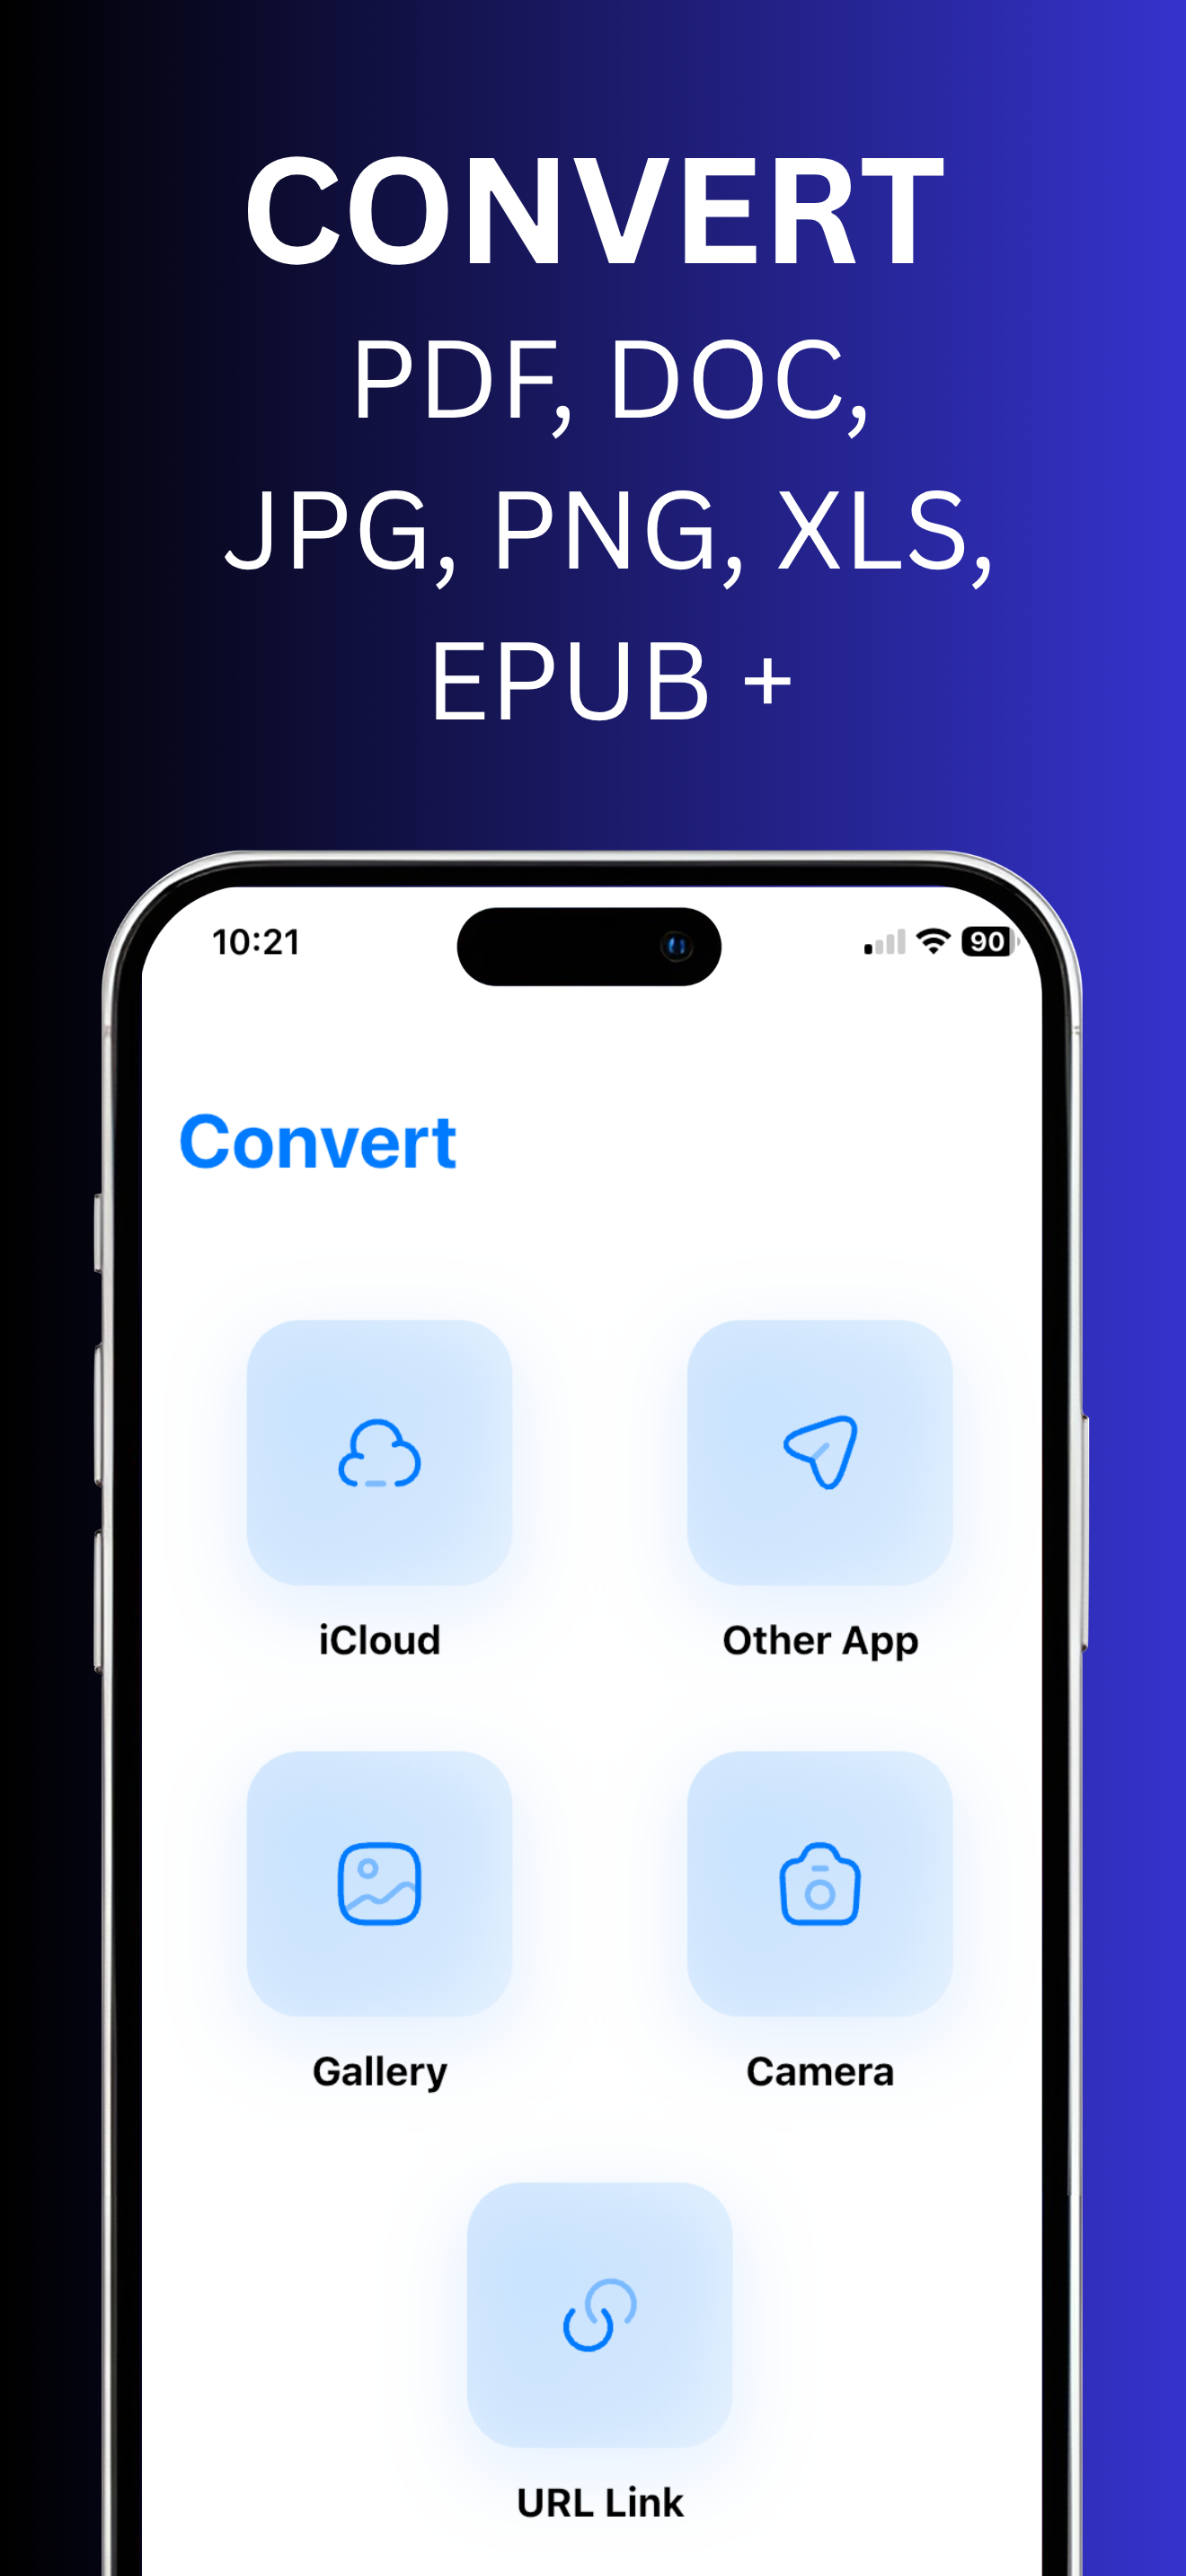
\includegraphics[width=\textwidth]{screenshots/3.png}\\
    \vspace{0.1cm}
    \scriptsize Chọn nguồn
\end{minipage}
\hfill
\begin{minipage}[b]{0.18\textwidth}
    \centering
    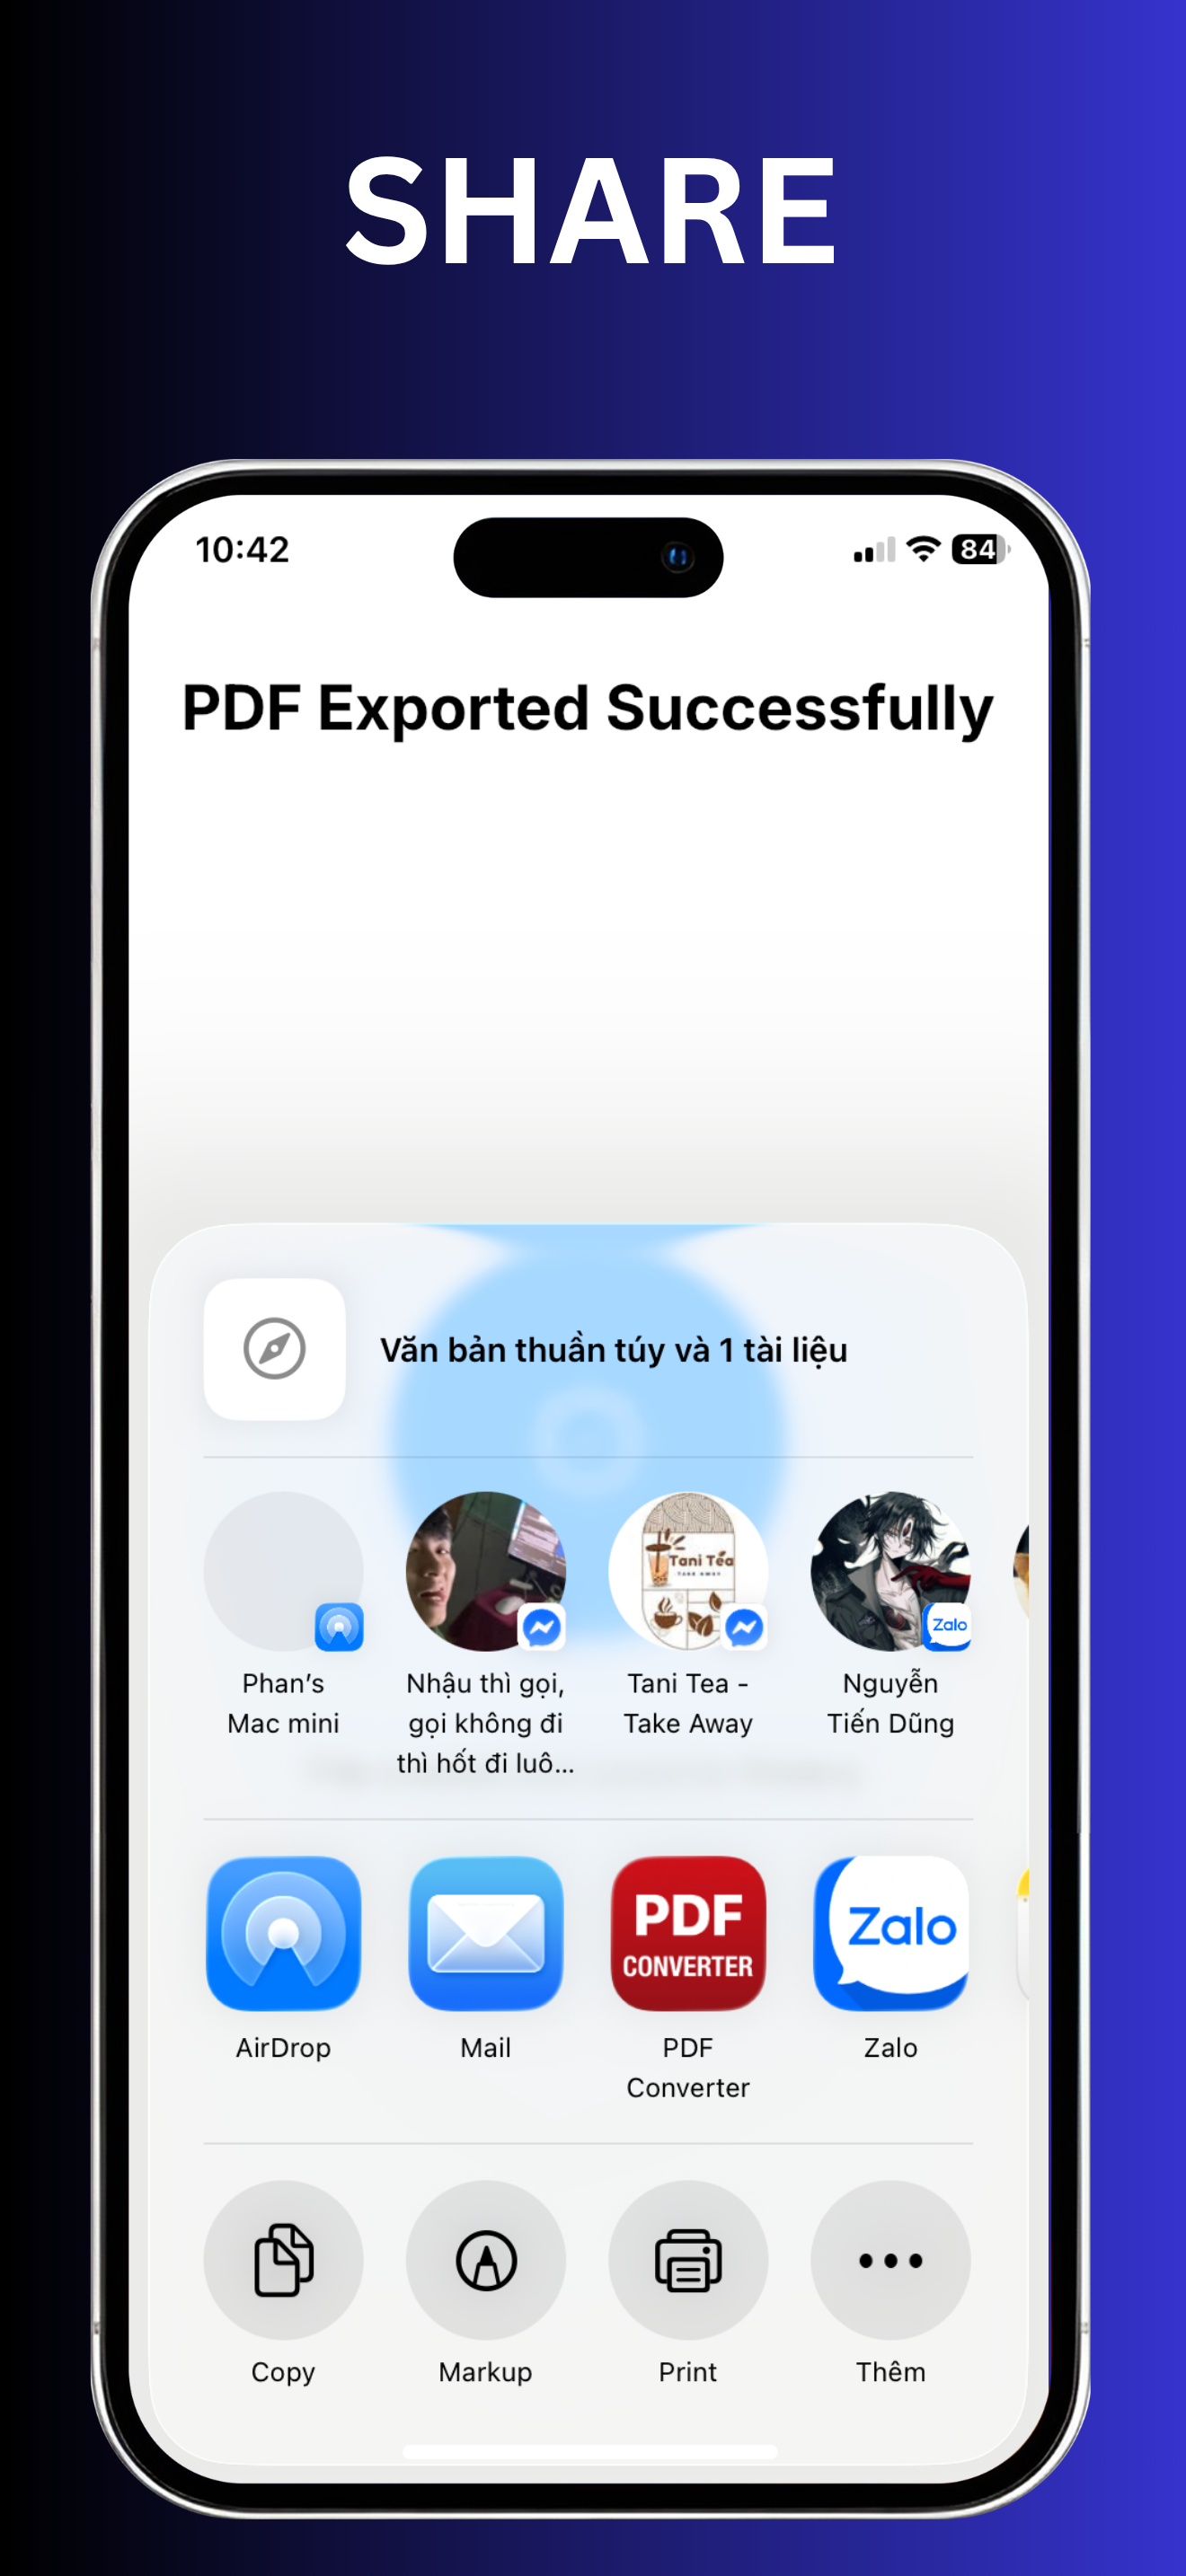
\includegraphics[width=\textwidth]{screenshots/4.png}\\
    \vspace{0.1cm}
    \scriptsize Xuất tệp PDF
\end{minipage}
\hfill
\begin{minipage}[b]{0.18\textwidth}
    \centering
    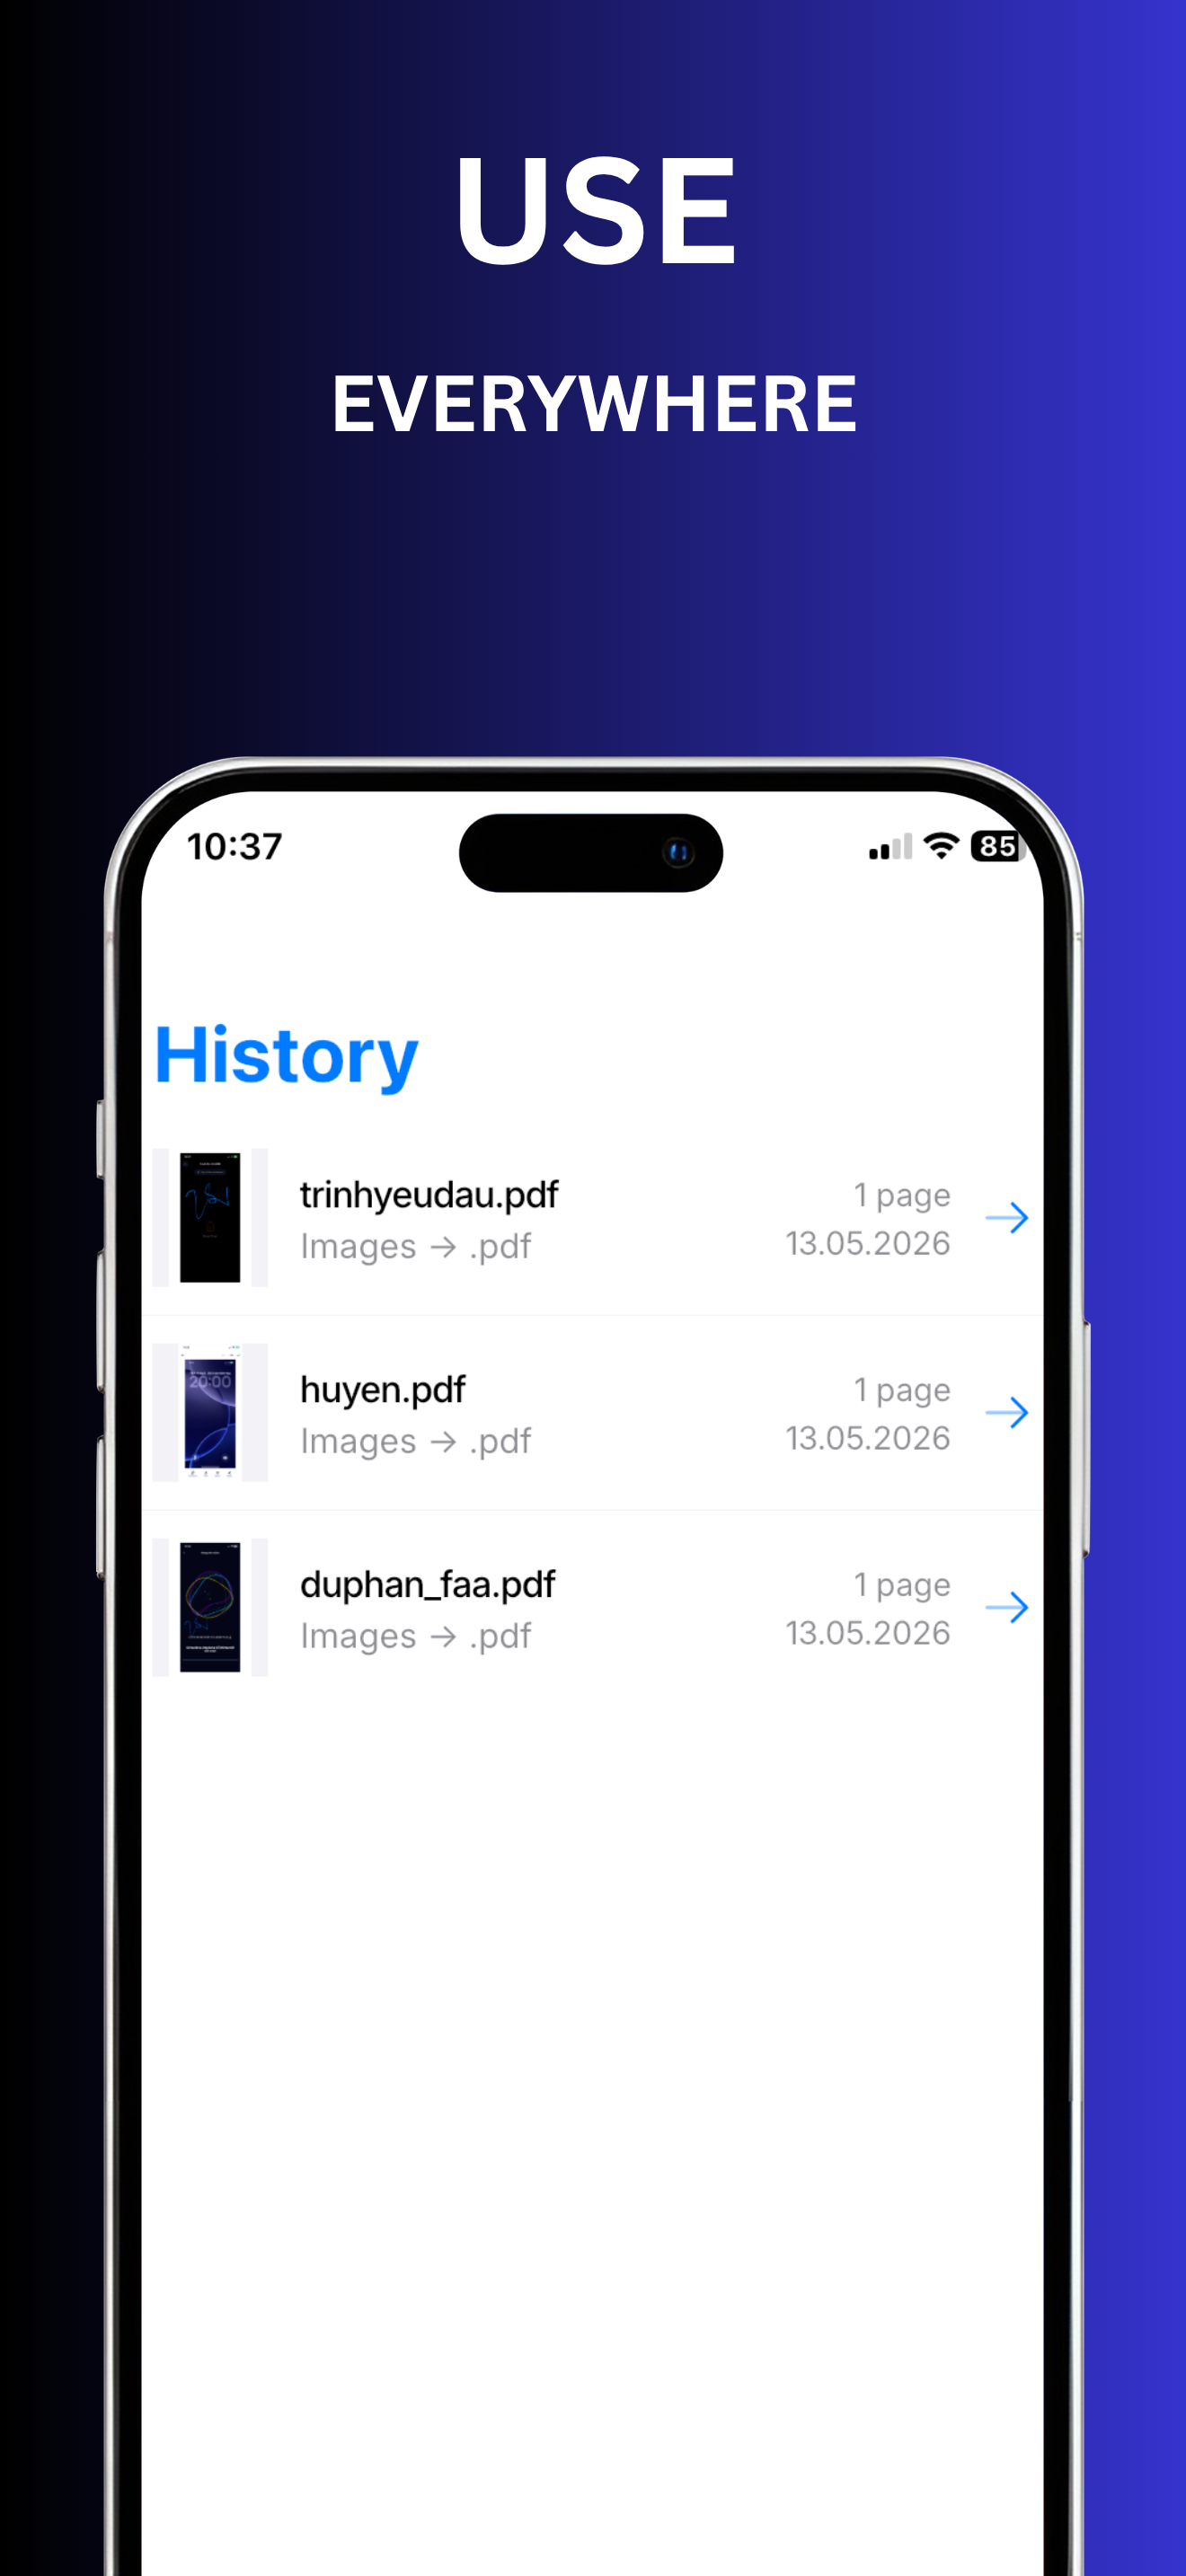
\includegraphics[width=\textwidth]{screenshots/5.png}\\
    \vspace{0.1cm}
    \scriptsize Lịch sử lưu
\end{minipage}
\caption{Giao diện thực tế của ứng dụng PDF Converter \& Scanner trên hệ điều hành iOS}
\label{fig:pdf_converter_screenshots}
\end{figure}


\subsubsection{Dự án Cleaner Guru - Tối ưu hóa doanh thu quảng cáo (Ads Optimization)}
\begin{itemize}
    \item \textbf{Tối ưu hóa AdMob SDK:} Nghiên cứu tích hợp quảng cáo Splash Ads và Interstitial Ads của Google AdMob, đảm bảo phân bổ hợp lý để không làm phiền trải nghiệm dọn dẹp kho ảnh của người dùng.
    \item \textbf{Khắc phục lỗi hiển thị quảng cáo:} Khắc phục triệt để lỗi quảng cáo Splash Ads đã được tải thành công và báo trạng thái sẵn sàng nhưng không thể trình chiếu do xung đột vòng đời Widget và xung đột luồng vẽ UI của Flutter. Tái cấu trúc lại cơ chế gọi callback bất đồng bộ an toàn giúp quảng cáo hiển thị mượt mà.
\end{itemize}
\subsubsection{Dự án Ad-Free Blood Pressure App - Phát hành và tối ưu tăng trưởng}
Đánh dấu mốc quan trọng khi đưa sản phẩm thực tế lên cửa hàng ứng dụng toàn cầu:
\begin{itemize}
    \item \textbf{Deploy thành công lên App Store:} Đổi tên chính thức dự án cá nhân ở giai đoạn 2 thành ứng dụng \textbf{Ad-Free Blood Pressure App} và hoàn tất các thủ tục phát hành thành công trên App Store tại đường dẫn: \url{https://apps.apple.com/us/app/ad-free-blood-pressure-app/id6749716071}.
    \item \textbf{Kết quả tăng trưởng đầu tiên:} Chỉ sau **1 tuần** xuất bản, ứng dụng đã xuất sắc đạt mốc **hơn 100 người dùng hoạt động** (organic users) tự nhiên.
\end{itemize}

\begin{figure}[htbp]
\centering
\begin{minipage}[b]{0.45\textwidth}
    \centering
    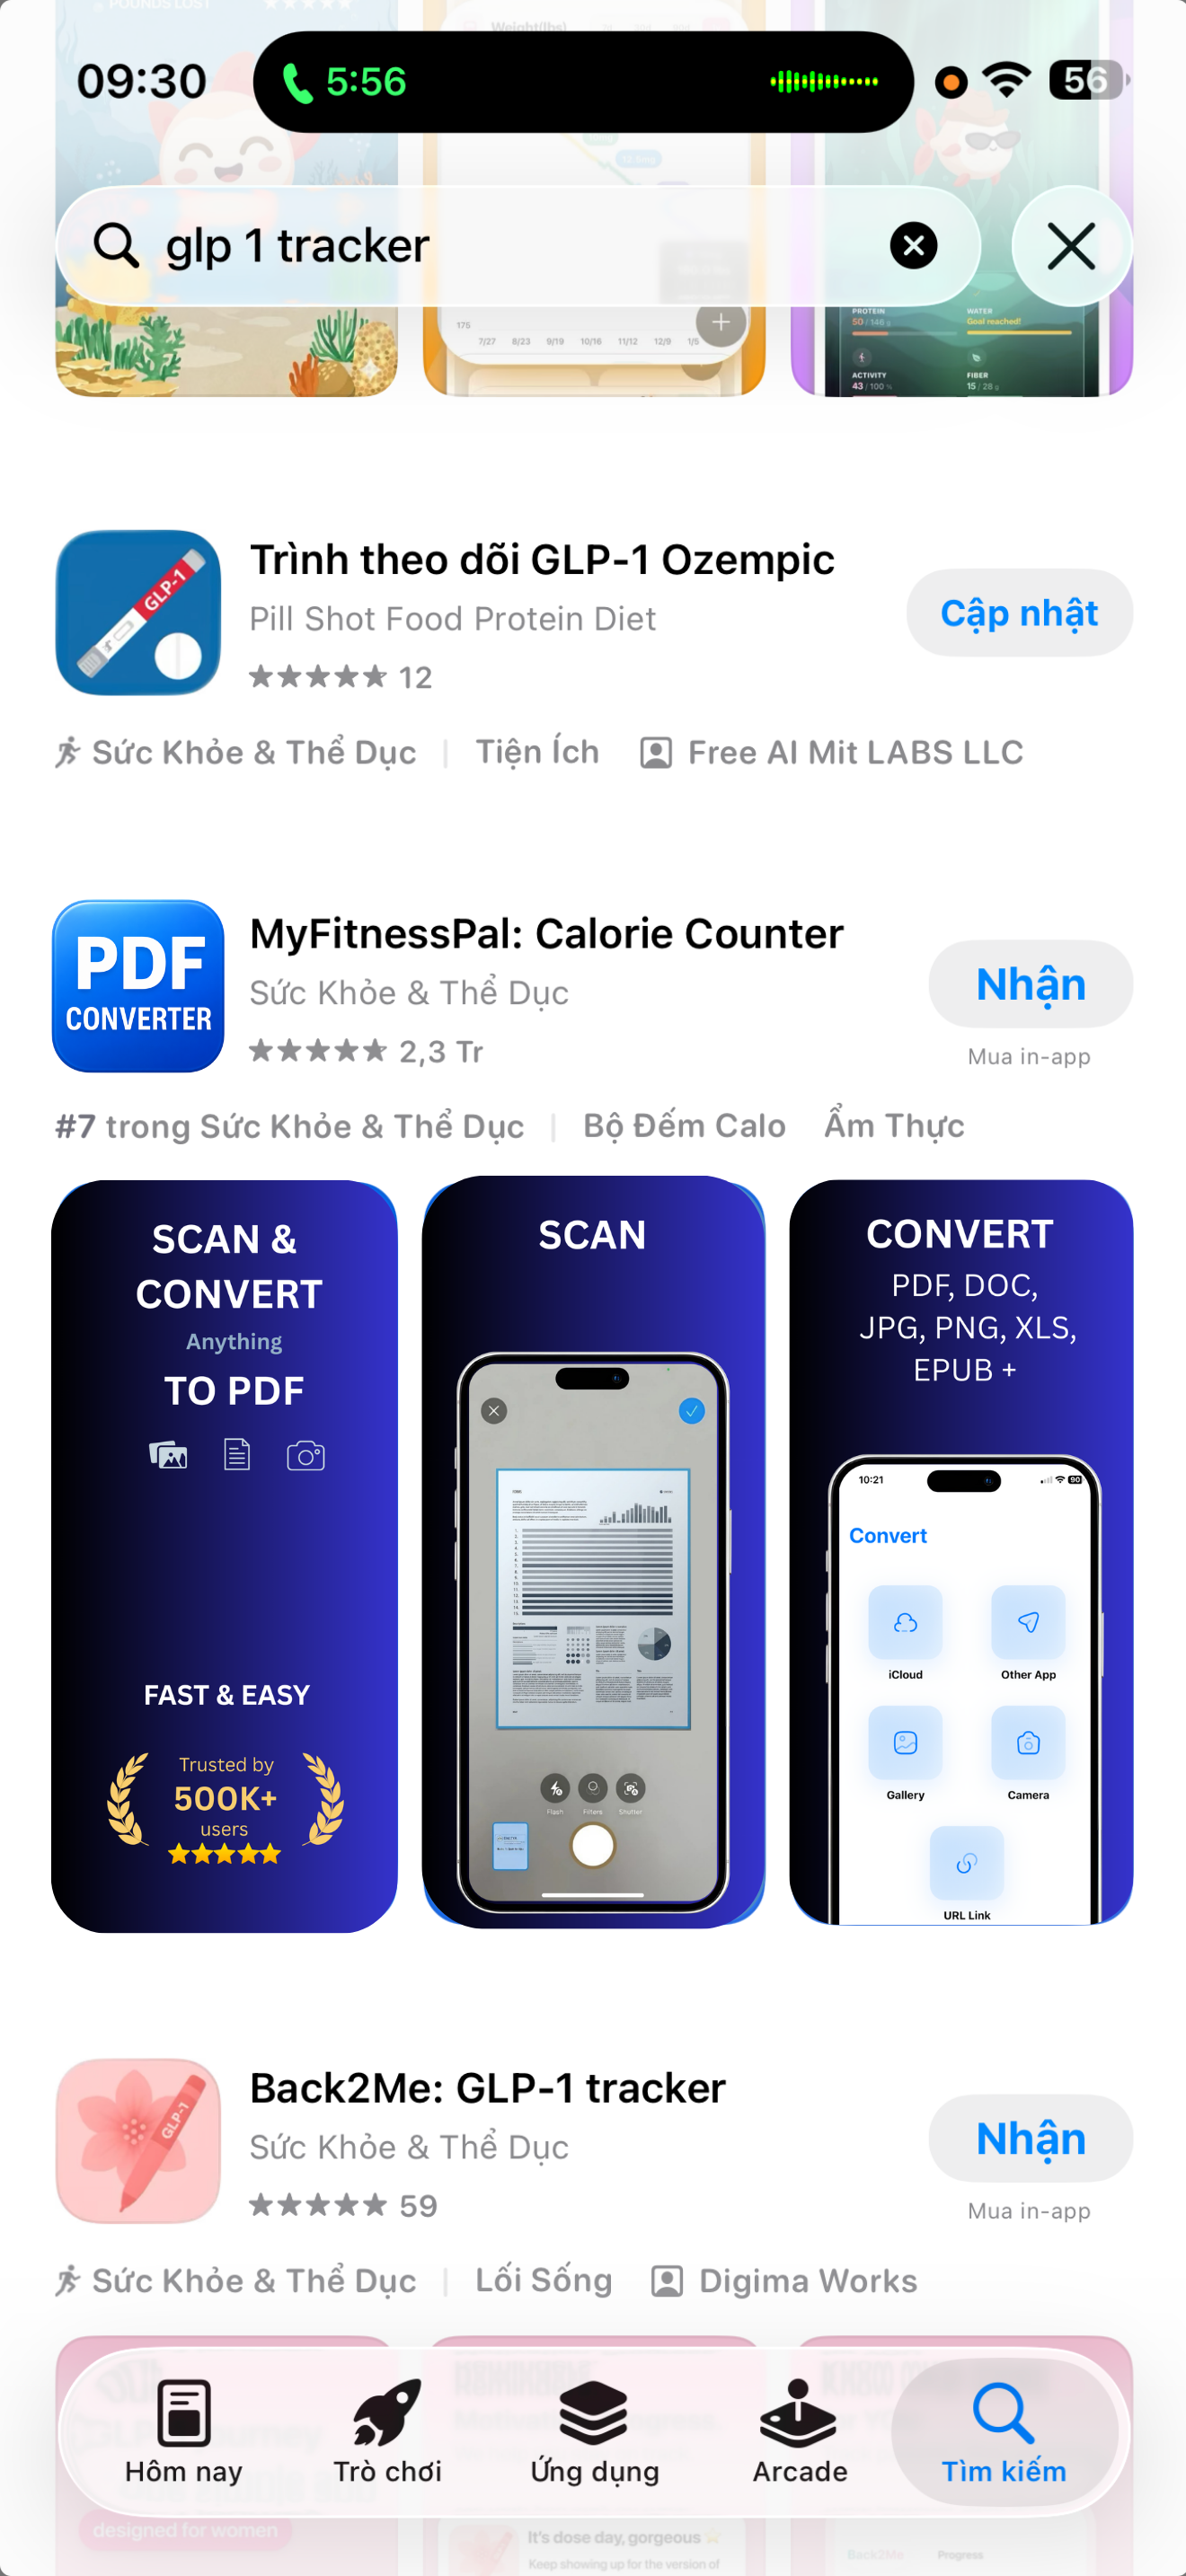
\includegraphics[width=\textwidth]{demo_app_store/1.png}\\
    \vspace{0.1cm}
    \scriptsize Giao diện App Store (Chế độ Sáng)
\end{minipage}
\hfill
\begin{minipage}[b]{0.45\textwidth}
    \centering
    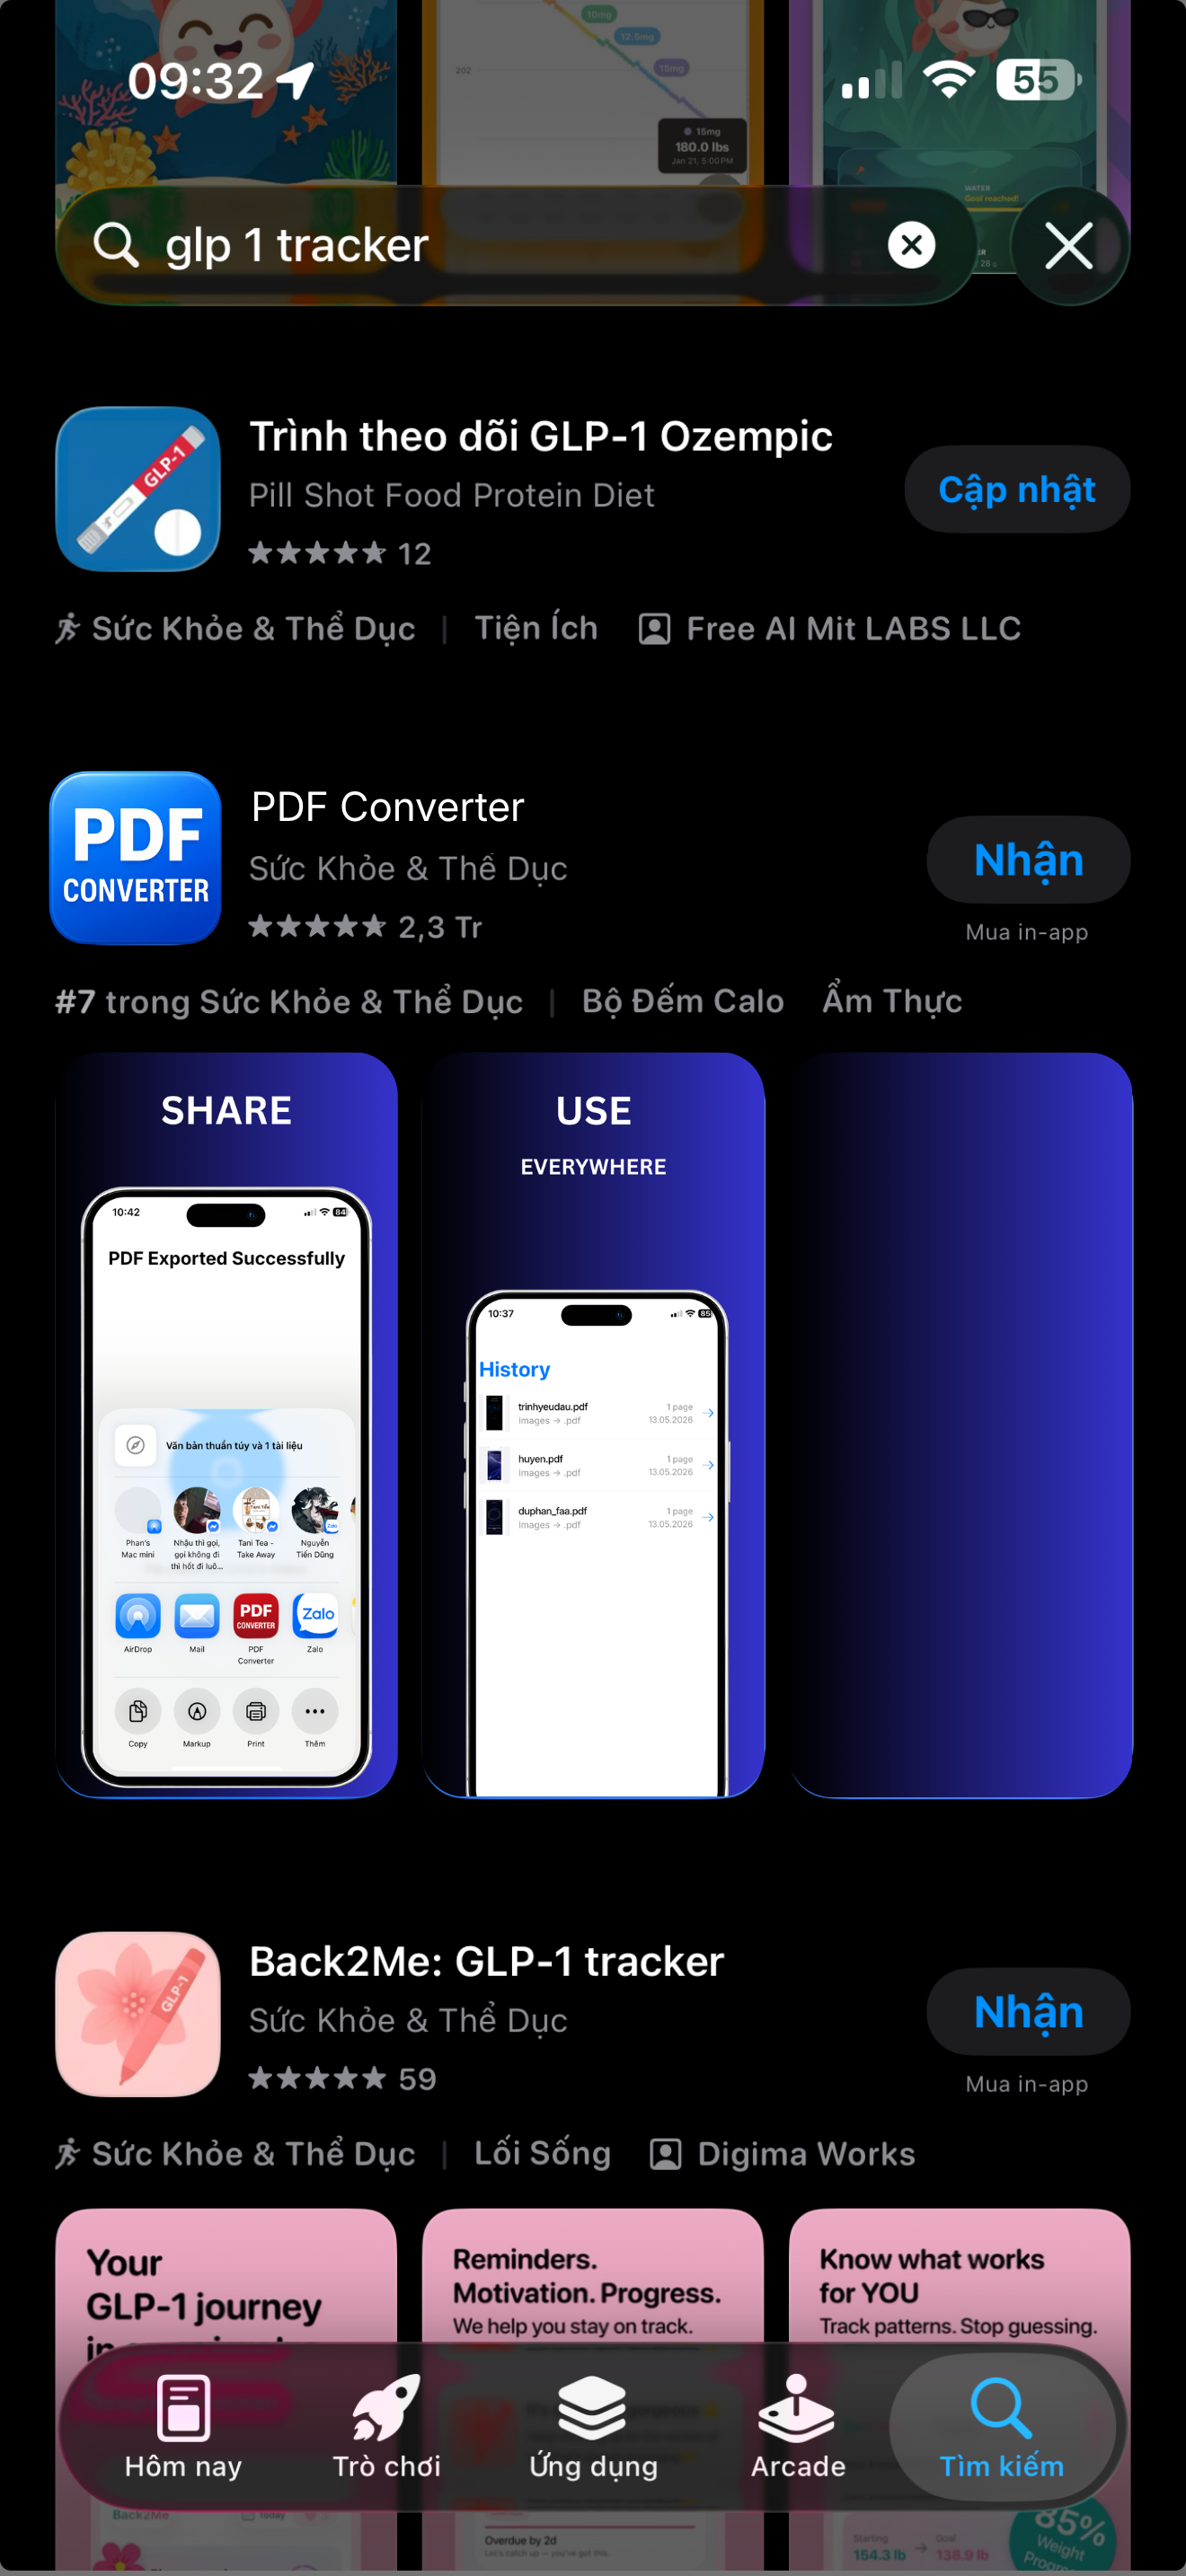
\includegraphics[width=\textwidth]{demo_app_store/2.png}\\
    \vspace{0.1cm}
    \scriptsize Giao diện App Store (Chế độ Tối)
\end{minipage}
\caption{Hình ảnh hiển thị thực tế của ứng dụng trên cửa hàng App Store}
\label{fig:app_store_screenshots}
\end{figure}


\subsection[Giai đoạn 5: Kiểm thử, Tối ưu hóa hệ thống và Báo cáo (Từ 21/05/2026 đến nay)]{Giai đoạn 5: Kiểm thử, Tối ưu hóa hệ thống và Báo cáo \\(Từ 21/05/2026 $\rightarrow$ Nay)}
\subsubsection{Công việc cụ thể}
\begin{itemize}
    \item \textbf{1. Hỗ trợ kiểm thử và khắc phục các vấn đề tương thích (QA Support):}
    Em phối hợp chặt chẽ với đội ngũ tester để tiến hành kiểm thử toàn diện các ứng dụng đã phát triển. Em tham gia phát hiện và khắc phục các vấn đề liên quan đến tương thích kích thước màn hình trên nhiều dòng máy iOS, tối ưu hóa kích thước ứng dụng và kiểm tra hiệu năng chạy ngầm để đảm bảo ứng dụng không bị hệ điều hành tắt khi đang quét.
    
    \item \textbf{2. Hoàn thiện hồ sơ báo cáo thực tập:}
    Em tổng kết toàn bộ tiến trình thực tập kéo dài hơn một năm tại FAA Việt Nam, đóng gói tài liệu kỹ thuật và hoàn thiện báo cáo thực tập tốt nghiệp chính thức để chuẩn bị báo cáo trước hội đồng nhà trường.
\end{itemize}
\subsubsection{Kết quả đạt được}
\begin{itemize}
    \item Các ứng dụng đạt độ ổn định cao trên môi trường kiểm thử, sẵn sàng cho các chiến dịch phát hành tiếp theo.
    \item Hoàn thành đầy đủ hồ sơ báo cáo thực tập chi tiết và chuẩn chỉ.
\end{itemize}

\section{TỰ ĐÁNH GIÁ VÀ BÀI HỌC KINH NGHIỆM}

\subsection{Điểm mạnh đạt được và Sự trưởng thành về chuyên môn}
Trải qua hơn một năm thực tập và làm việc thực tế tại FAA Việt Nam dưới sự chỉ dẫn tận tình và chuyên nghiệp của Mentor Phan Bá Đủ, em đã đạt được sự trưởng thành vượt bậc cả về năng lực kỹ thuật lẫn tác phong làm việc:
\begin{itemize}
    \item \textbf{Năng lực chuyên môn vững vàng:} Làm chủ thành thạo các kỹ thuật lập trình Flutter nâng cao: quản lý luồng ngầm bất đồng bộ (Isolate), lập trình giao tiếp đa nền tảng Method Channel để gọi thư viện Native, triển khai kiến trúc chuẩn Clean Architecture, sử dụng cơ chế quản lý trạng thái Flutter Bloc chuyên nghiệp và tối ưu hóa hệ thống cơ sở dữ liệu Isar DB.
    \item \textbf{Nghiên cứu và ứng dụng công nghệ hiện đại:} Nghiên cứu thành công và đưa vào thực tế các thuật toán sinh trắc học phức tạp (PPG đo nhịp tim), trí tuệ nhân tạo thị giác máy tính (MediaPipe nhận diện tư thế người), thuật toán so khớp ảnh dHash và bộ phân tích cấu trúc tài liệu Office Open XML (OOXML) offline.
    \item \textbf{Tư duy hướng sản phẩm thương mại:} Tự mình thực hiện quy trình phát hành thành công ứng dụng Ad-Free Blood Pressure App lên App Store toàn cầu, tối ưu hóa hiển thị và doanh thu quảng cáo SDK Google AdMob mang lại hiệu quả kinh doanh thực tế cho doanh nghiệp.
    \item \textbf{Tác phong lập trình hiện đại:} Sử dụng nhuần nhuyễn các công cụ AI hỗ trợ lập trình (Cursor AI) theo phương pháp Vibe Coding giúp tăng 40% hiệu suất làm việc mà vẫn đảm bảo tính an toàn và chất lượng của mã nguồn.
\end{itemize}

\subsection{Hạn chế cần tiếp tục hoàn thiện}
Bên cạnh những thành tích đã đạt được, em cũng thẳng thắn nhìn nhận những điểm hạn chế cần nỗ lực khắc phục trong tương lai:
\begin{itemize}
    \item \textbf{Hạn chế của thuật toán trên thiết bị phần cứng yếu:} Thuật toán đo nhịp tim qua PPG camera và thuật toán nhận diện tư thế qua MediaPipe vẫn có tỉ lệ sai số nhất định khi chạy trên các dòng máy cấu hình cũ hoặc trong môi trường thiếu sáng, camera bị rung lắc mạnh.
    \item \textbf{Kỹ năng viết tài liệu thiết kế hệ thống (System Design Doc):} Việc biểu diễn các cấu trúc hệ thống phức tạp thông qua các sơ đồ (Diagram) vẫn cần tiếp tục trau dồi để có thể truyền đạt thiết kế kỹ thuật một cách trực quan và dễ hiểu nhất cho các thành viên trong dự án.
\end{itemize}

\subsection{Bài học kinh nghiệm rút ra}
Kỳ thực tập kéo dài hơn một năm tại FAA Việt Nam là trải nghiệm vô cùng quý giá, giúp em đúc kết được những bài học quan trọng:
\begin{itemize}
    \item \textbf{Kiến trúc Clean Architecture và Clean Code:} Là xương sống cho bất kỳ dự án phần mềm lớn nào. Viết mã nguồn sạch, dễ đọc và dễ bảo trì giúp tiết kiệm hàng trăm giờ làm việc của nhóm khi dự án nâng cấp tính năng.
    \item \textbf{Quy trình Git Flow và Code Review chéo:} Là lá chắn bảo vệ sự ổn định của hệ thống. Mọi Pull Request đều cần được xem xét cẩn trọng để phát hiện sớm các lỗi logic trước khi đưa sản phẩm đến tay khách hàng.
    \item \textbf{Trách nhiệm với sản phẩm và tập thể:} Thói quen bám sát tiến độ trên Jira, chủ động thảo luận các vấn đề kỹ thuật với Mentor và hỗ trợ nhiệt tình đội ngũ QA trong quá trình kiểm thử hộp đen/hộp trắng là những yếu tố quyết định tạo nên thành công của dự án.
\end{itemize}

\section{KẾT QUẢ TỔNG THỂ VÀ KẾT LUẬN}
\begin{itemize}
    \item \textbf{Kết quả:} Tham gia phát triển thành công 5 ứng dụng di động thực tế bao gồm: \textit{Blood Sugar, Ad-Free Blood Pressure App, Cleaner Guru, Push Up, và PDF Converter \& Scanner}. Trong đó, em đã độc lập phát hành ứng dụng \textbf{Ad-Free Blood Pressure App} lên App Store toàn cầu và đạt mốc trên 100 người dùng hoạt động tự nhiên sau 1 tuần. Đảm đương tốt tất cả các module có độ phức tạp cao của doanh nghiệp dưới sự hướng dẫn của Mentor Phan Bá Đủ.
    \item \textbf{Bài học kinh nghiệm quý báu:} Đợt thực tập hơn 1 năm tại FAA Việt Nam đã rèn luyện cho em tư duy thiết kế phần mềm sạch (Clean Code), viết mã dễ bảo trì và luôn hướng tới trải nghiệm tốt nhất cho người dùng cuối cùng.
    \item \textbf{Định hướng nghề nghiệp:} Phấn đấu trở thành Senior Mobile Developer tại FAA Việt Nam, tiếp tục nghiên cứu sâu về các giải pháp học máy và trí tuệ nhân tạo trên thiết bị di động (On-device AI).
\end{itemize}

\newpage
\section*{PHỤ LỤC: HÌNH ẢNH MINH HỌA GIAO DIỆN ỨNG DỤNG}
\addcontentsline{toc}{section}{PHỤ LỤC: HÌNH ẢNH MINH HỌA GIAO DIỆN ỨNG DỤNG}
Dưới đây là toàn bộ hình ảnh giao diện thực tế ghi nhận kết quả phát triển các ứng dụng di động trong suốt giai đoạn thực tập tính đến ngày 20/05/2026:

\subsection*{Phần 1: Dự án Cleaner Guru (Giai đoạn 2)}
Ứng dụng dọn dẹp ảnh trùng lặp thông minh, giải phóng dung lượng bộ nhớ thiết bị iOS:

\subsubsection*{1.1. Màn hình Onboarding}
\begin{figure}[htbp]
    \centering
    \begin{minipage}{0.45\textwidth}
        \centering
        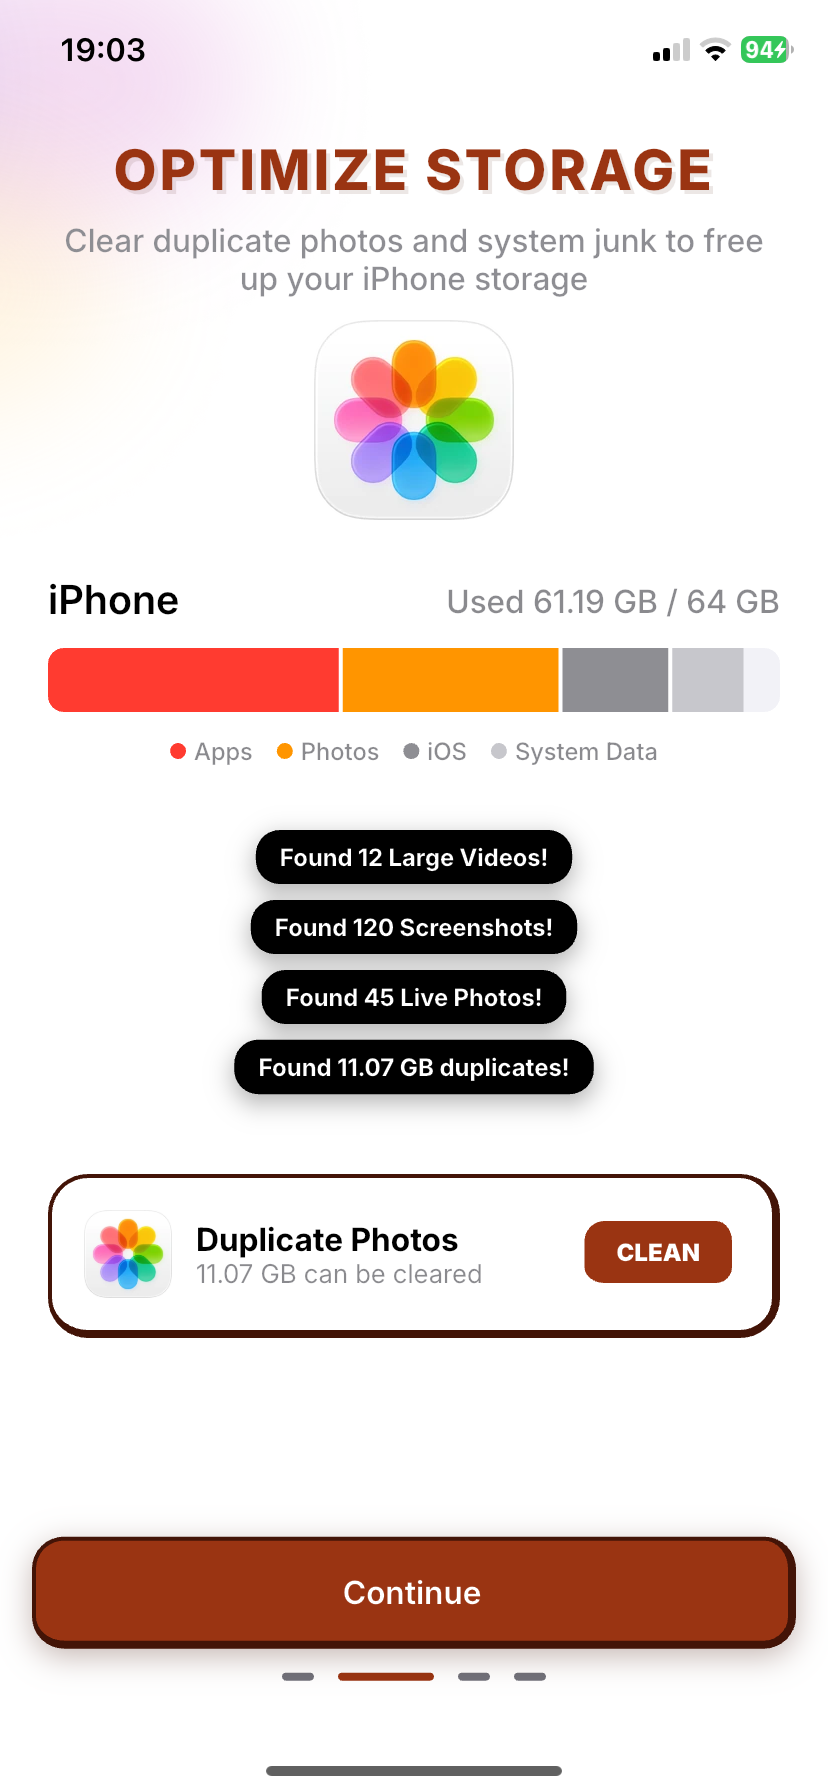
\includegraphics[height=9.5cm]{cleanerguru/IMG_6851.PNG}
        \caption{Onboarding: Giới thiệu tính năng phân tích bộ nhớ lưu trữ.}
        \label{fig:cleaner_onb_storage}
    \end{minipage}
    \hfill
    \begin{minipage}{0.45\textwidth}
        \centering
        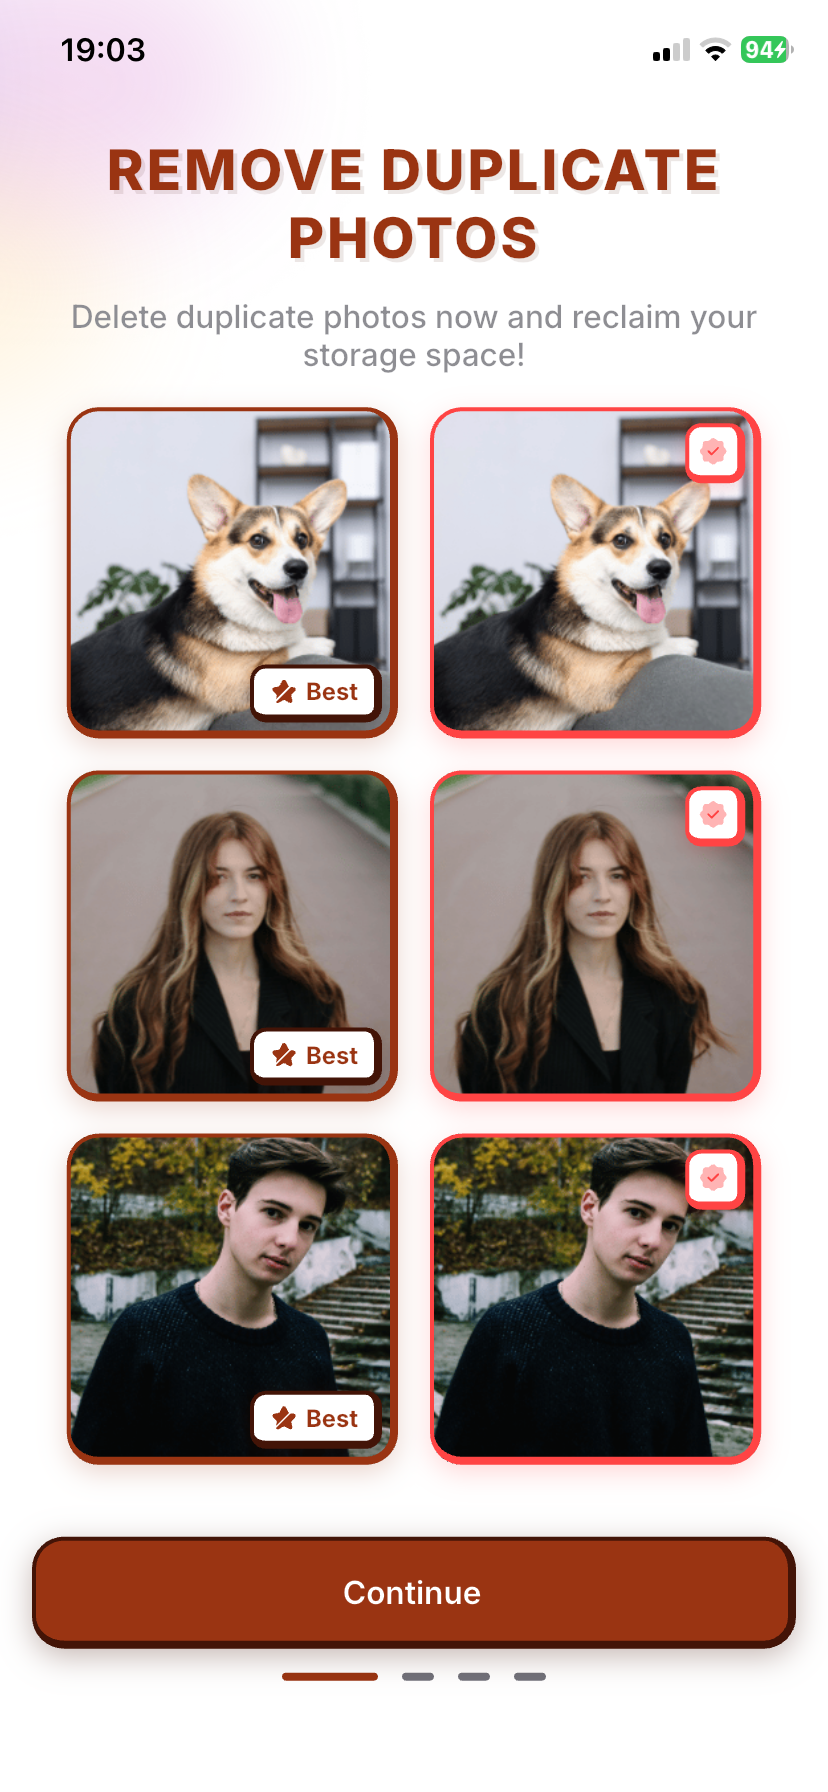
\includegraphics[height=9.5cm]{cleanerguru/IMG_6850.PNG}
        \caption{Onboarding: Giới thiệu tính năng gom nhóm ảnh tương đồng.}
        \label{fig:cleaner_onb_similar}
    \end{minipage}
\end{figure}

\begin{figure}[htbp]
    \centering
    \begin{minipage}{0.45\textwidth}
        \centering
        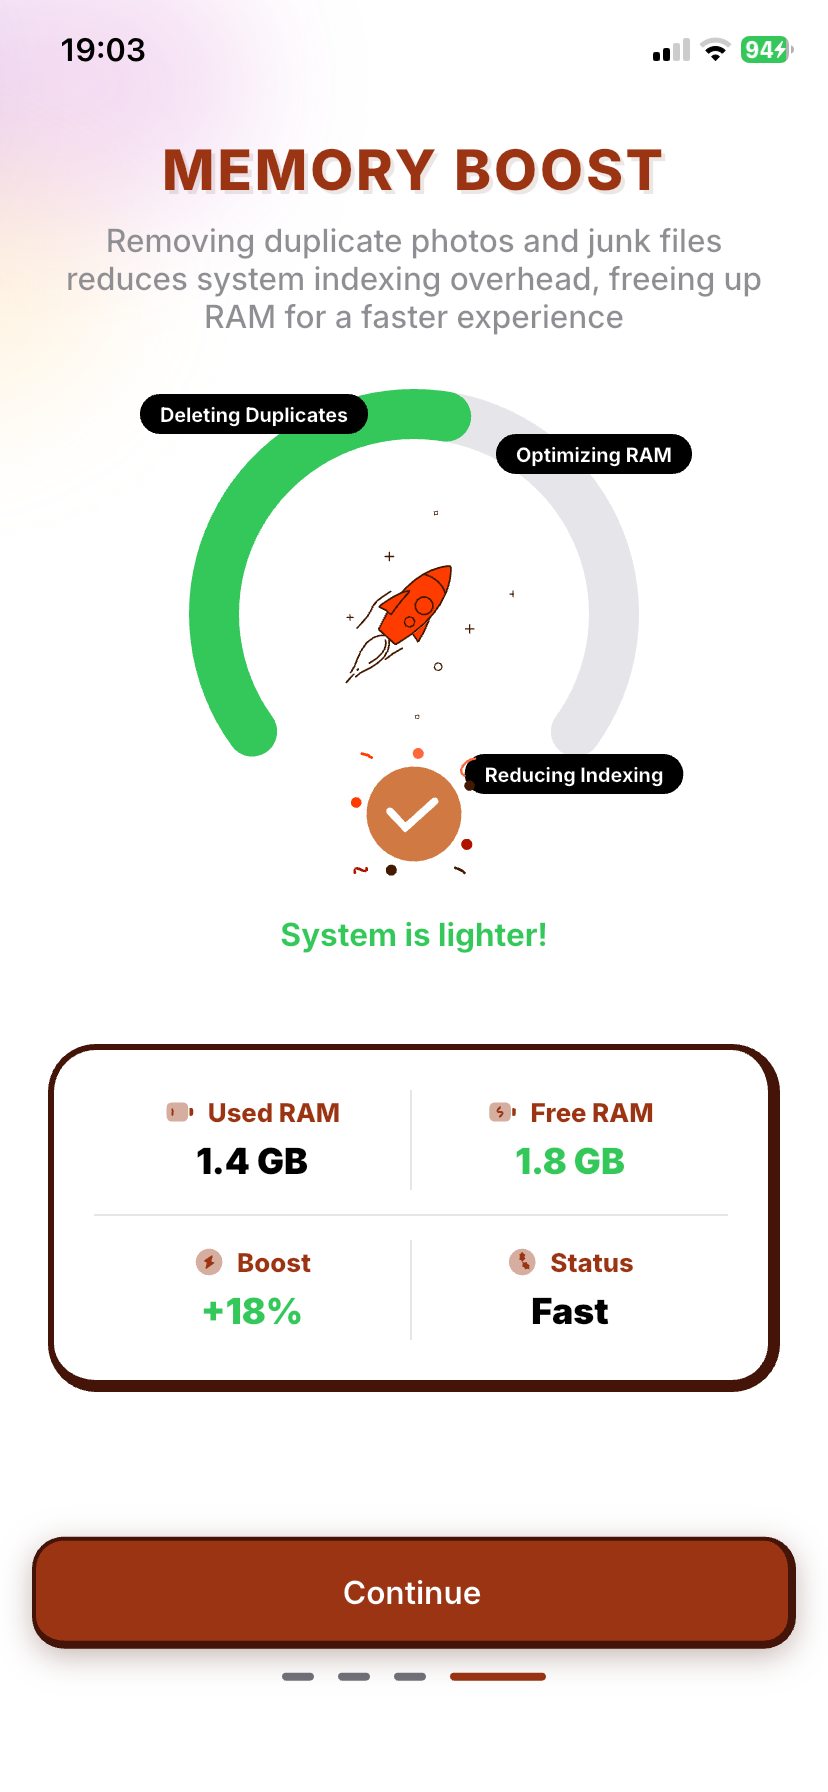
\includegraphics[height=9.5cm]{cleanerguru/IMG_6854.PNG}
        \caption{Onboarding: Giới thiệu tính năng Memory Boost (giải phóng RAM).}
        \label{fig:cleaner_onb_ram}
    \end{minipage}
    \hfill
    \begin{minipage}{0.45\textwidth}
        \centering
        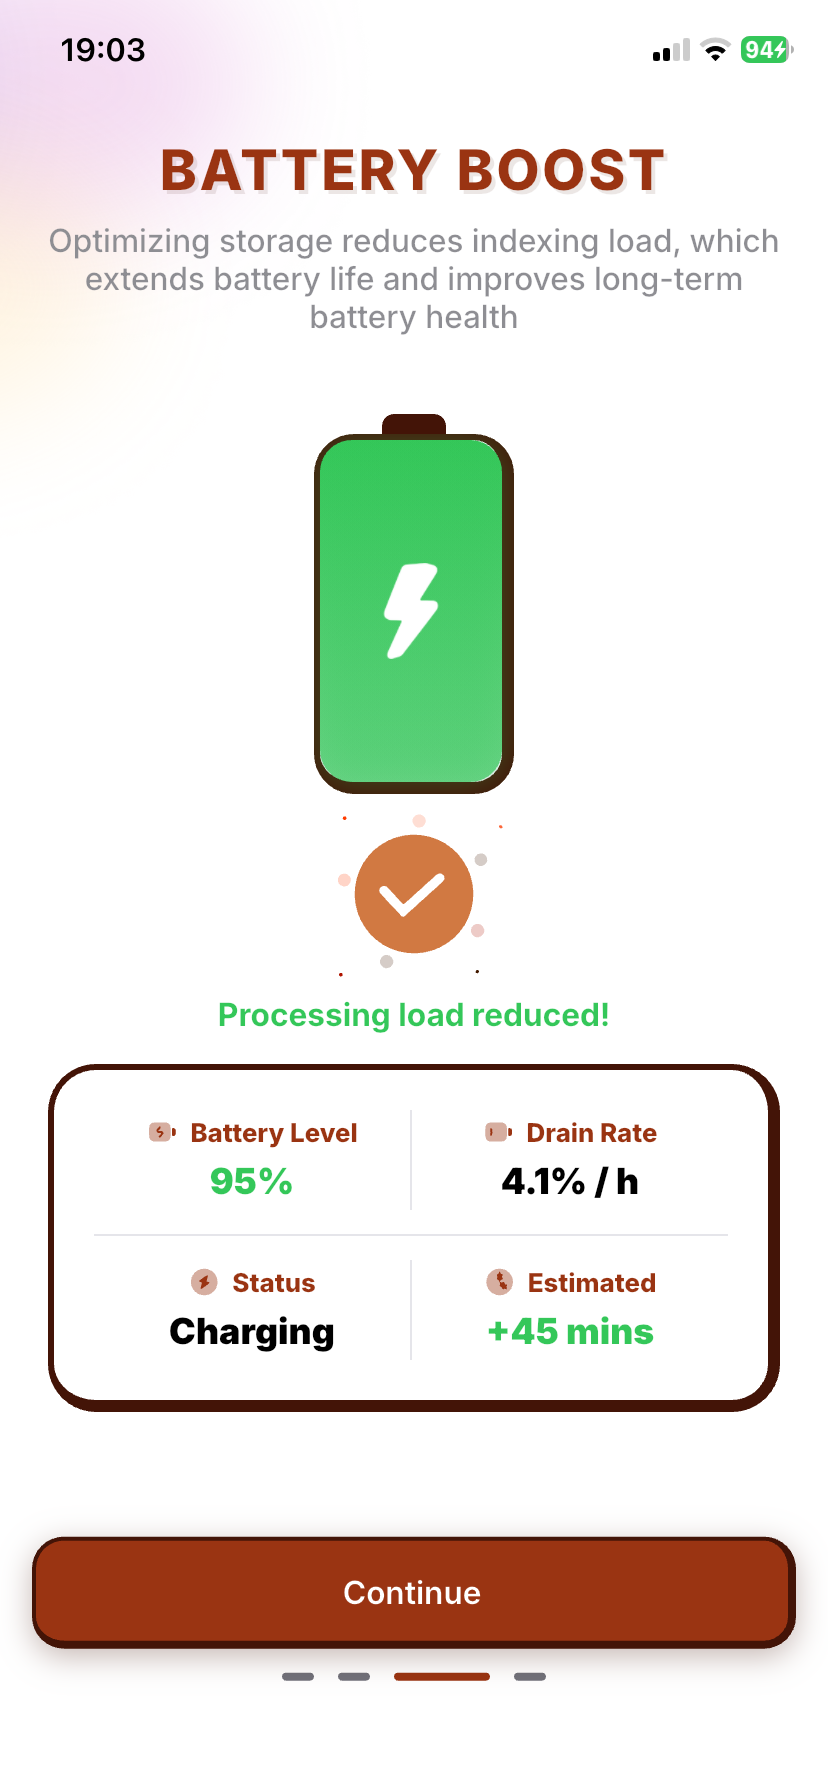
\includegraphics[height=9.5cm]{cleanerguru/IMG_6853.PNG}
        \caption{Onboarding: Giới thiệu tính năng Battery Boost (tối ưu pin).}
        \label{fig:cleaner_onb_battery}
    \end{minipage}
\end{figure}

\newpage
\subsubsection*{1.2. Màn hình Tính năng Chính}
\begin{figure}[htbp]
    \centering
    \begin{minipage}{0.45\textwidth}
        \centering
        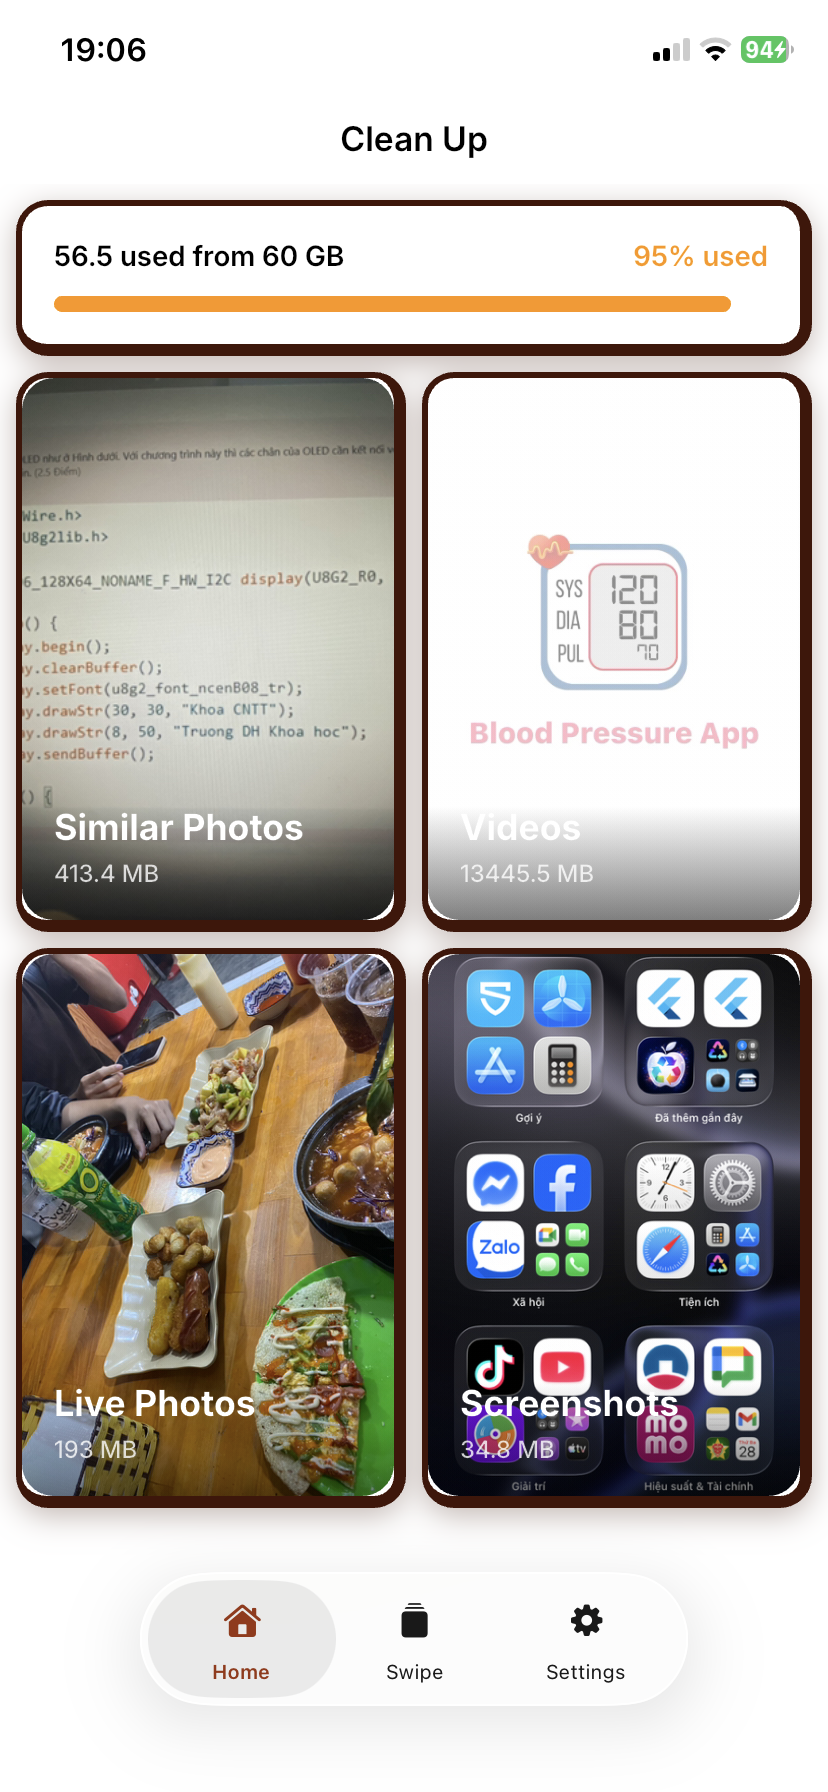
\includegraphics[height=9.5cm]{cleanerguru/IMG_6863.PNG}
        \caption{Màn hình chính Clean Up: phân loại ảnh giống nhau, video, live photo và screenshots theo dung lượng.}
        \label{fig:cleaner_home}
    \end{minipage}
    \hfill
    \begin{minipage}{0.45\textwidth}
        \centering
        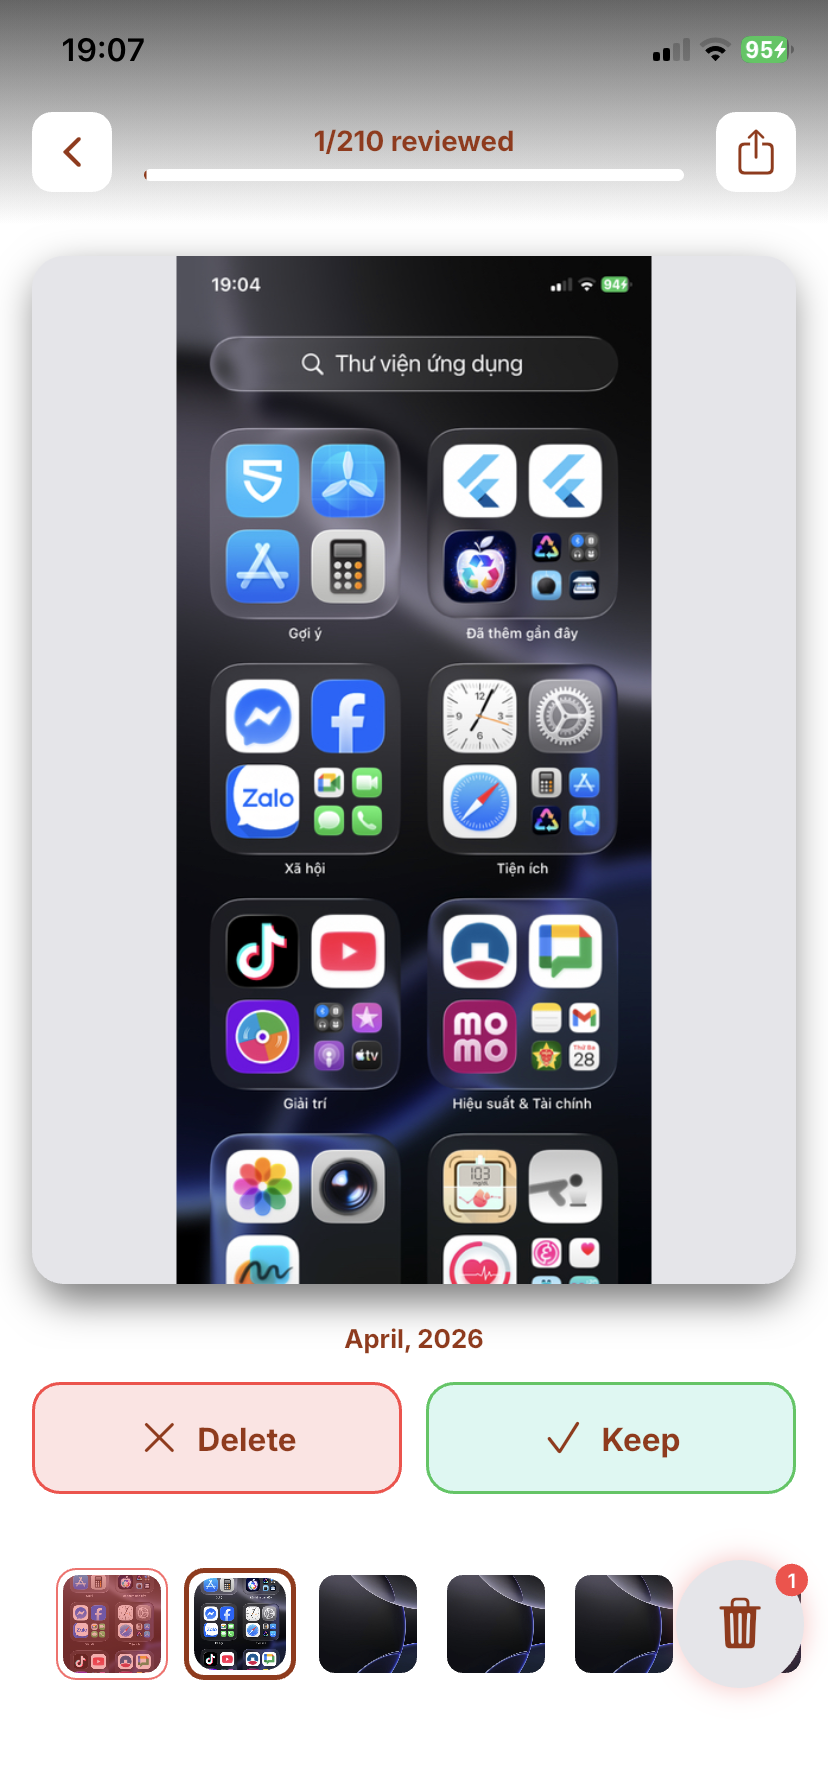
\includegraphics[height=9.5cm]{cleanerguru/IMG_6868.PNG}
        \caption{Giao diện Swipe Photos: đánh giá từng ảnh và chọn giữ lại hoặc xóa (Keep/Delete).}
        \label{fig:cleaner_review}
    \end{minipage}
\end{figure}

\begin{figure}[htbp]
    \centering
    \begin{minipage}{0.45\textwidth}
        \centering
        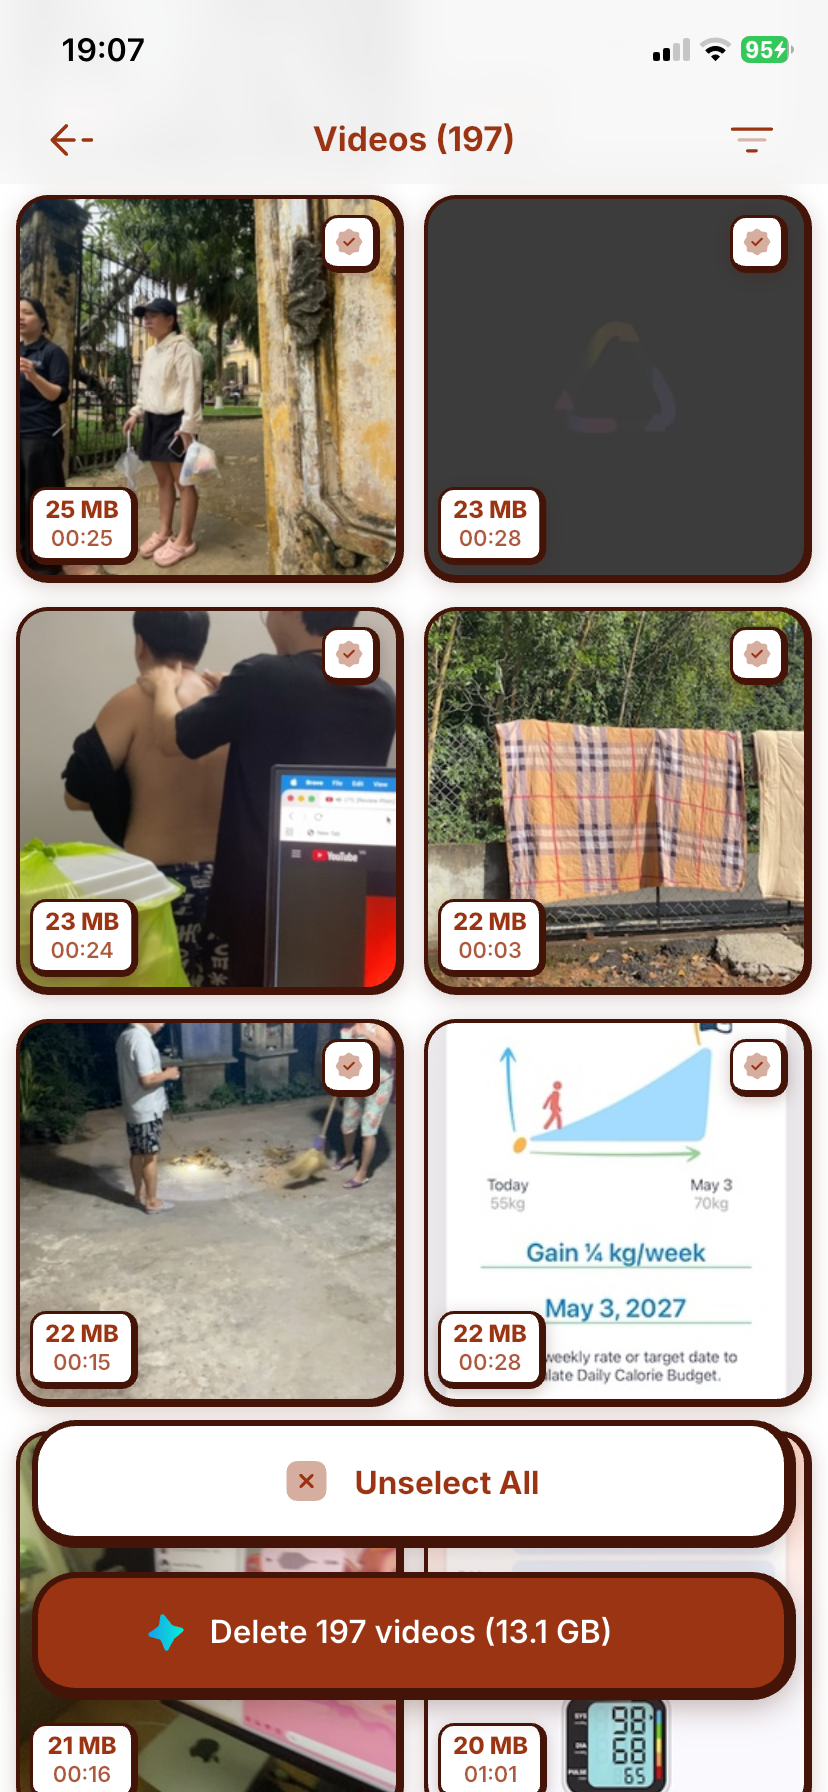
\includegraphics[height=9.5cm]{cleanerguru/IMG_6865.PNG}
        \caption{Màn hình dọn dẹp video dung lượng lớn (197 videos -- 13.1 GB).}
        \label{fig:cleaner_videos}
    \end{minipage}
    \hfill
    \begin{minipage}{0.45\textwidth}
        \centering
        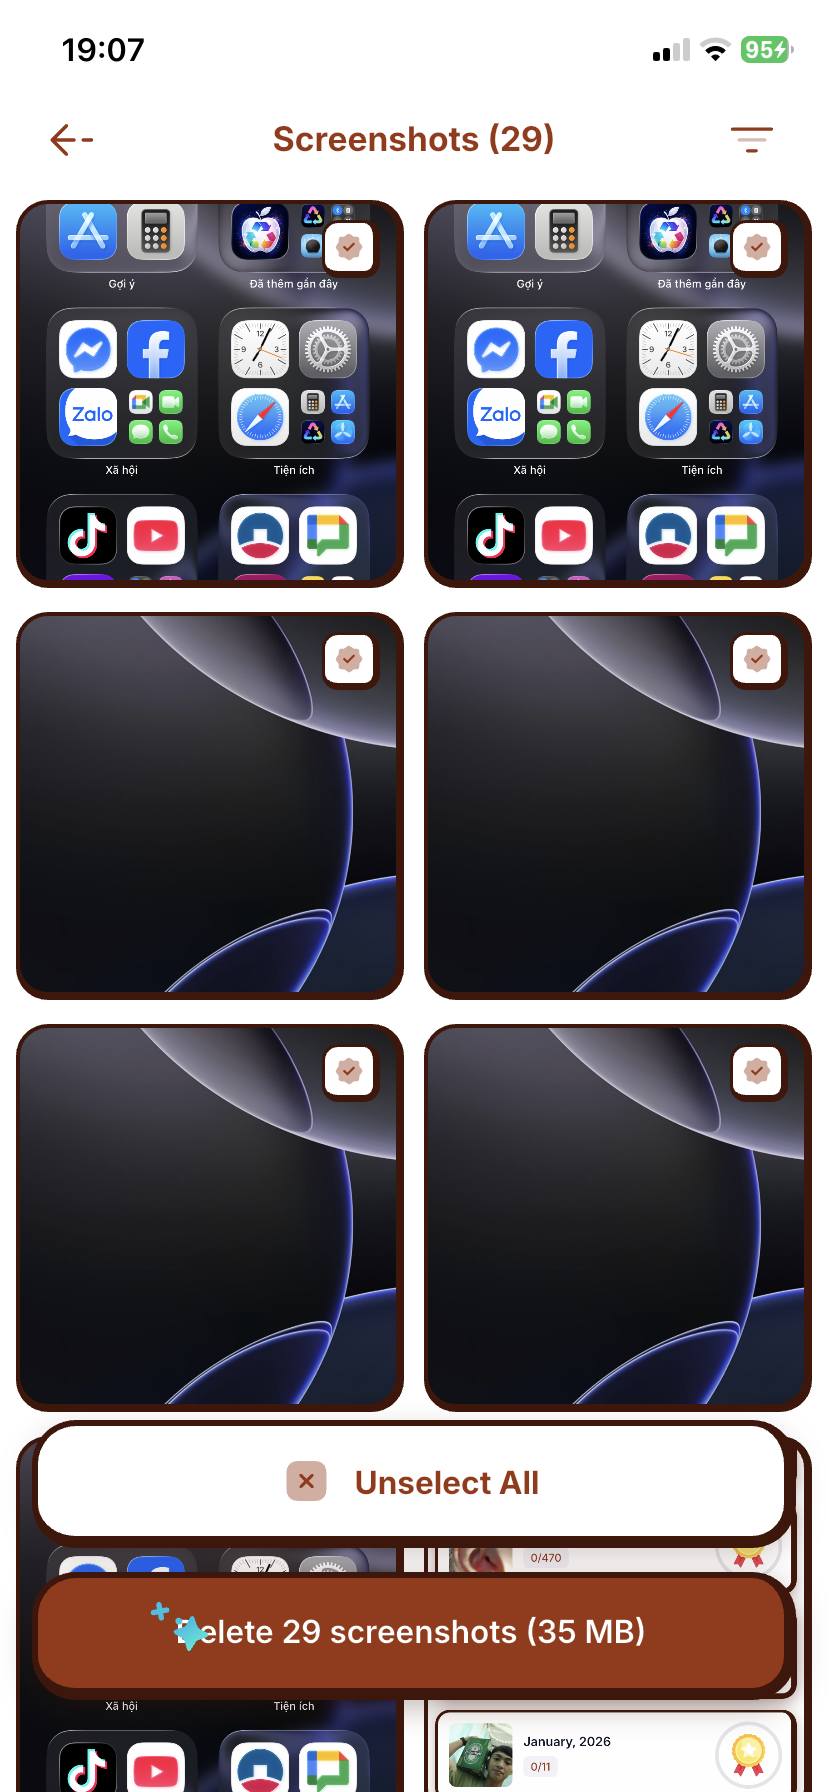
\includegraphics[height=9.5cm]{cleanerguru/IMG_6866.PNG}
        \caption{Màn hình xóa hàng loạt ảnh chụp màn hình trùng lặp (29 screenshots -- 35 MB).}
        \label{fig:cleaner_screenshots}
    \end{minipage}
\end{figure}

\newpage
\subsection*{Phần 2: Dự án Push Up (Giai đoạn 2)}
Ứng dụng hỗ trợ theo dõi sức khỏe và tự động đếm số lần hít đất sử dụng cảm biến tiệm cận:

\begin{figure}[htbp]
    \centering
    \begin{minipage}{0.45\textwidth}
        \centering
        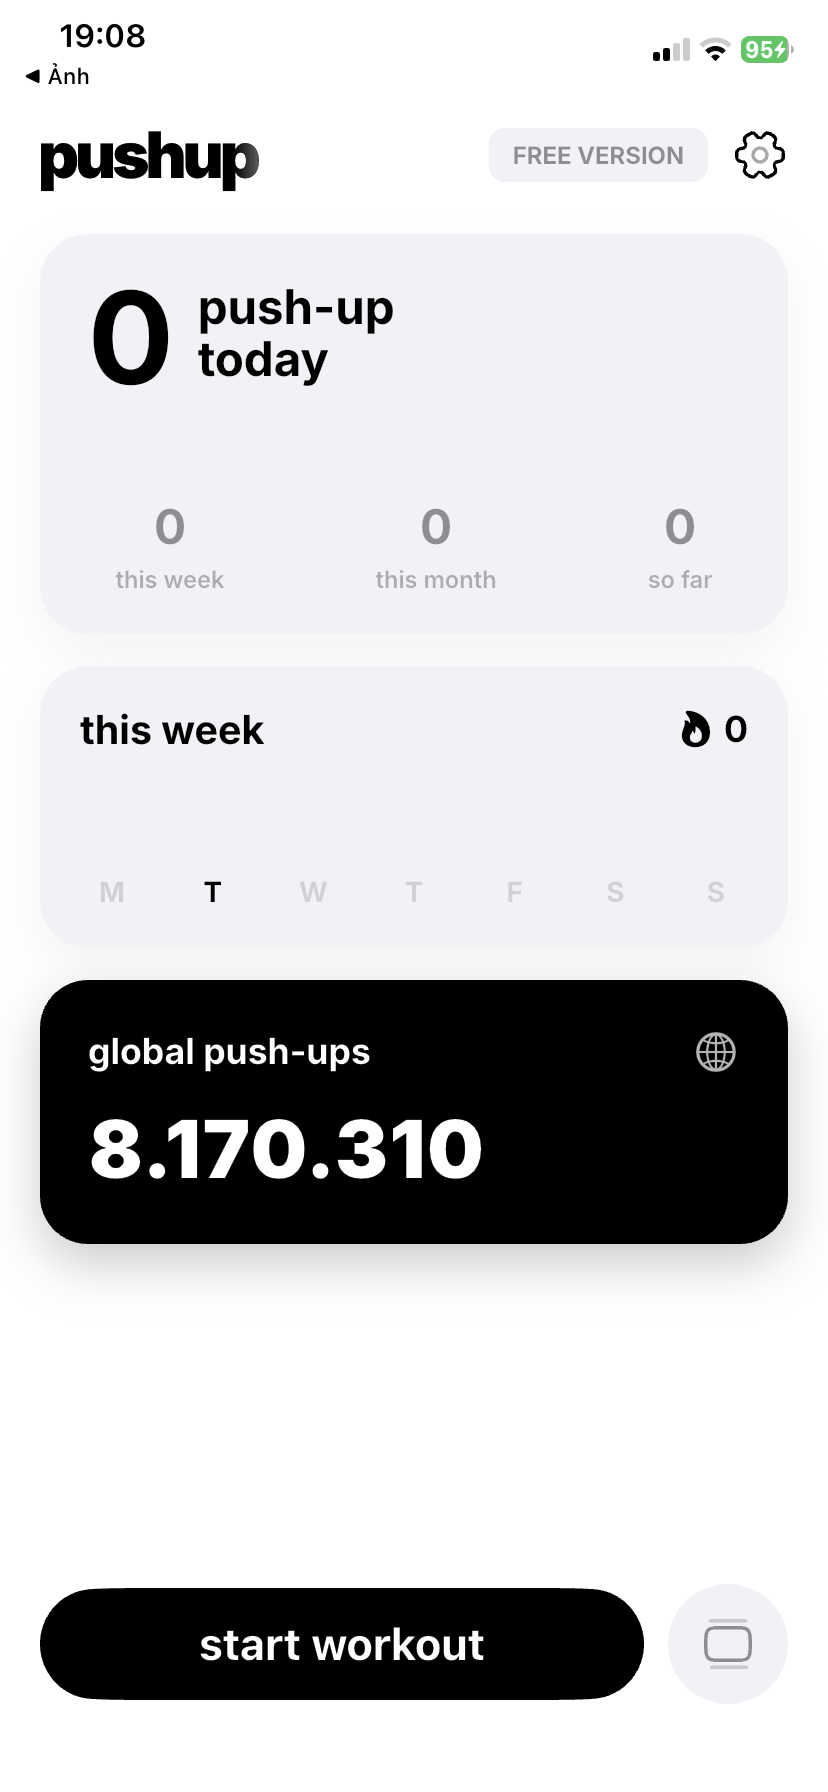
\includegraphics[height=9.5cm]{push_up/IMG_6870.PNG}
        \caption{Màn hình chính thống kê tập luyện (Dashboard).}
        \label{fig:pushup_dash}
    \end{minipage}
    \hfill
    \begin{minipage}{0.45\textwidth}
        \centering
        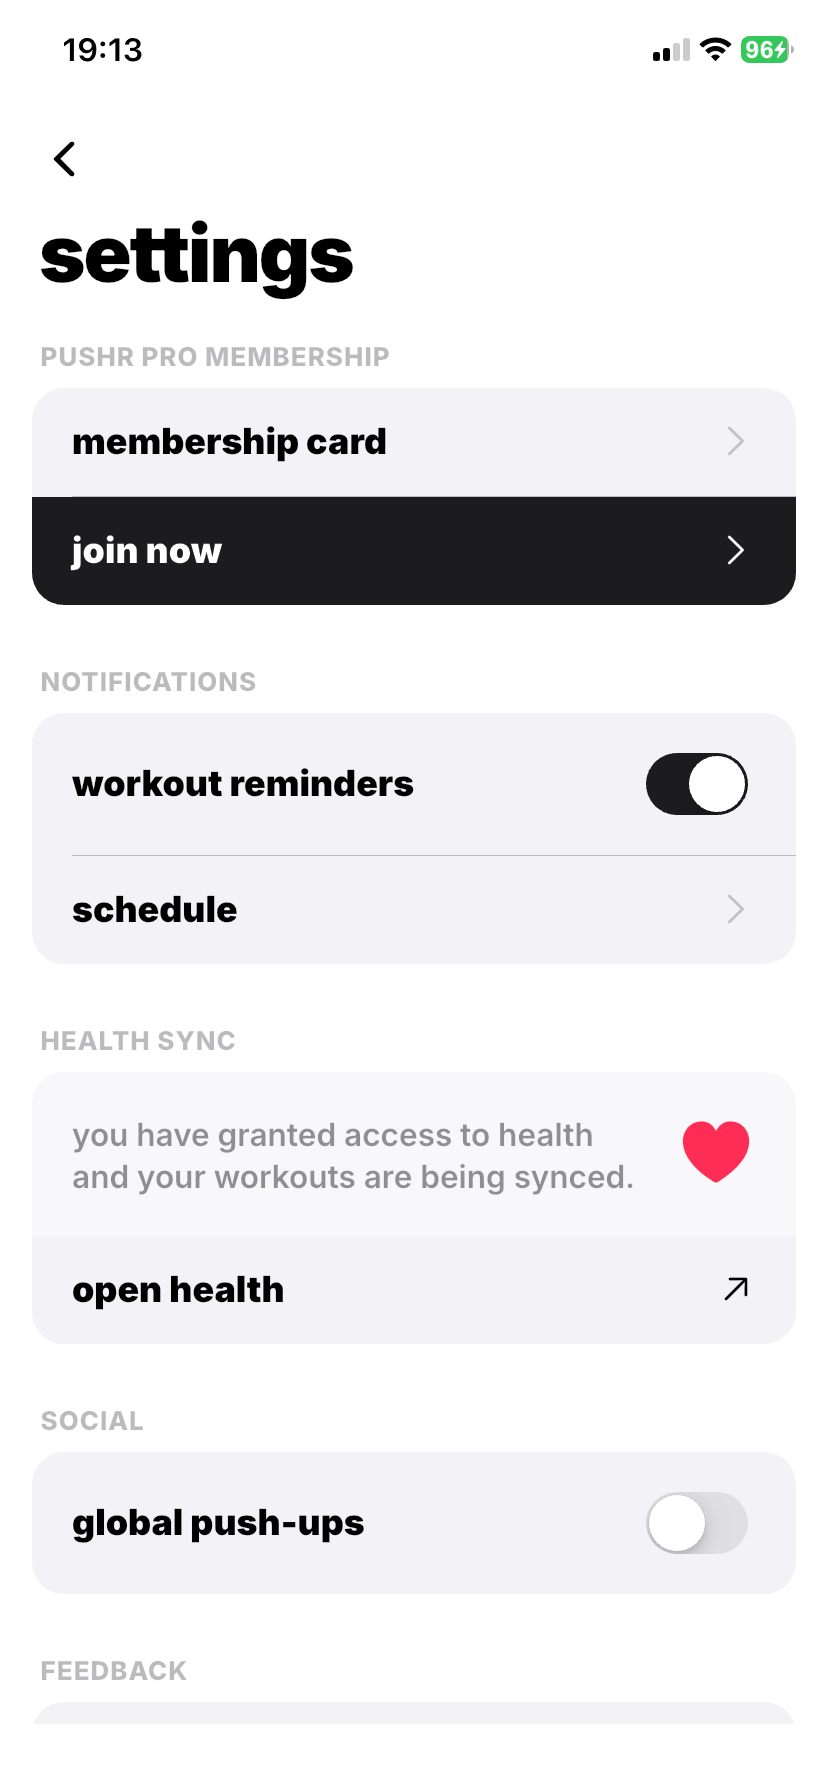
\includegraphics[height=9.5cm]{push_up/IMG_6876.PNG}
        \caption{Giao diện cấu hình và đồng bộ Health Sync.}
        \label{fig:pushup_settings}
    \end{minipage}
\end{figure}

\newpage
\begin{figure}[htbp]
    \centering
    \begin{minipage}{0.45\textwidth}
        \centering
        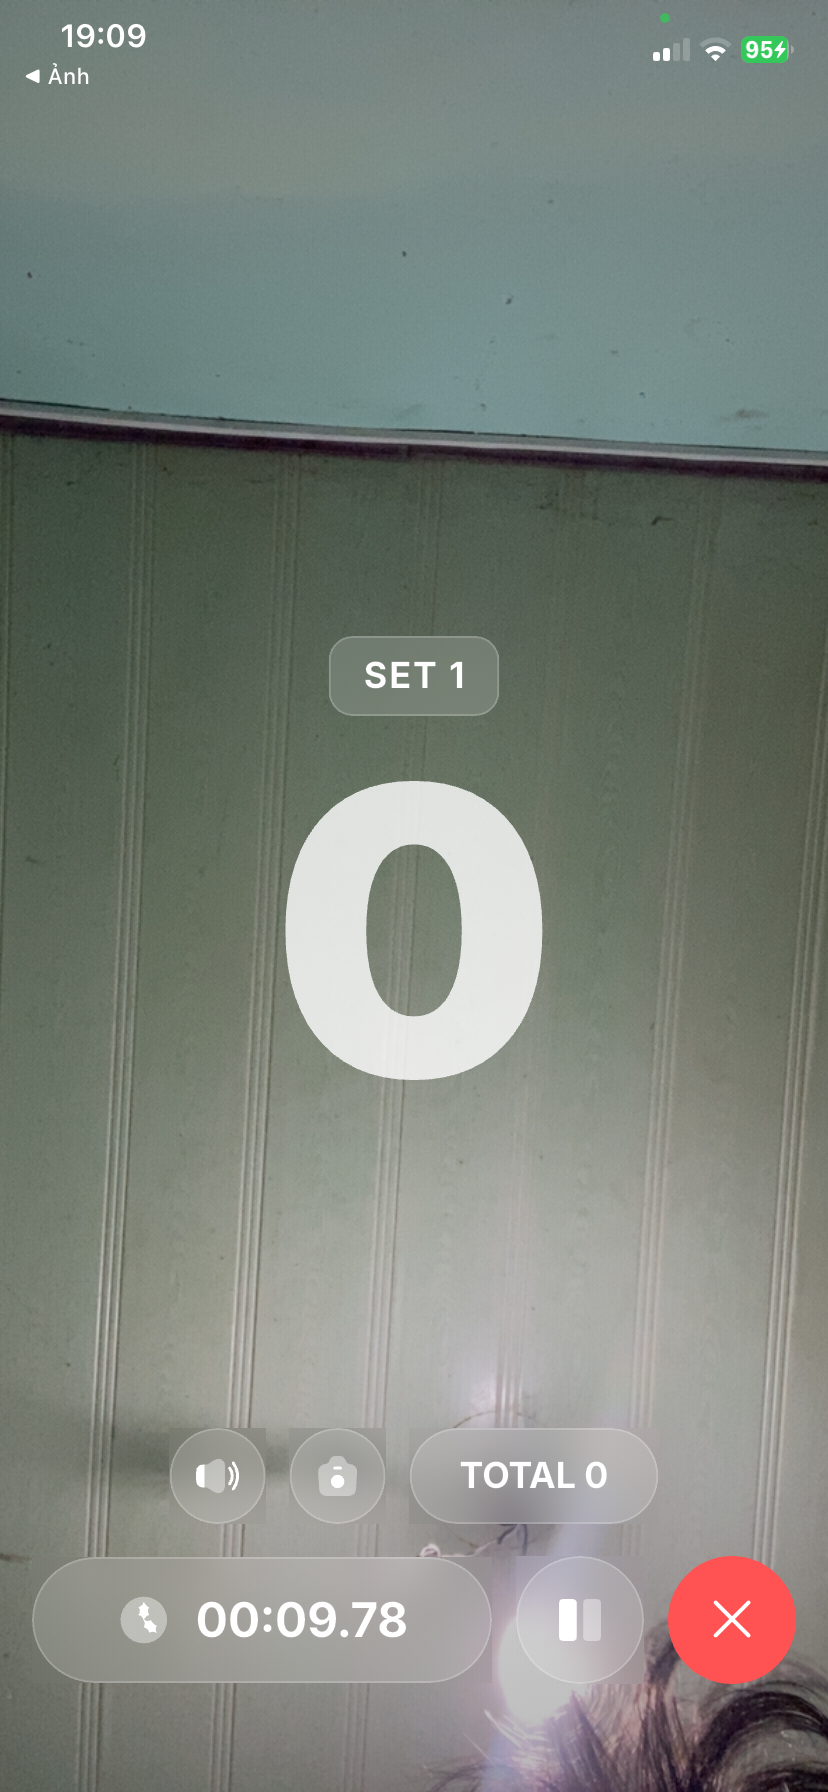
\includegraphics[height=9.5cm]{push_up/IMG_6871.PNG}
        \caption{Giao diện buổi tập hít đất (Start Workout).}
        \label{fig:pushup_work}
    \end{minipage}
    \hfill
    \begin{minipage}{0.45\textwidth}
        \centering
        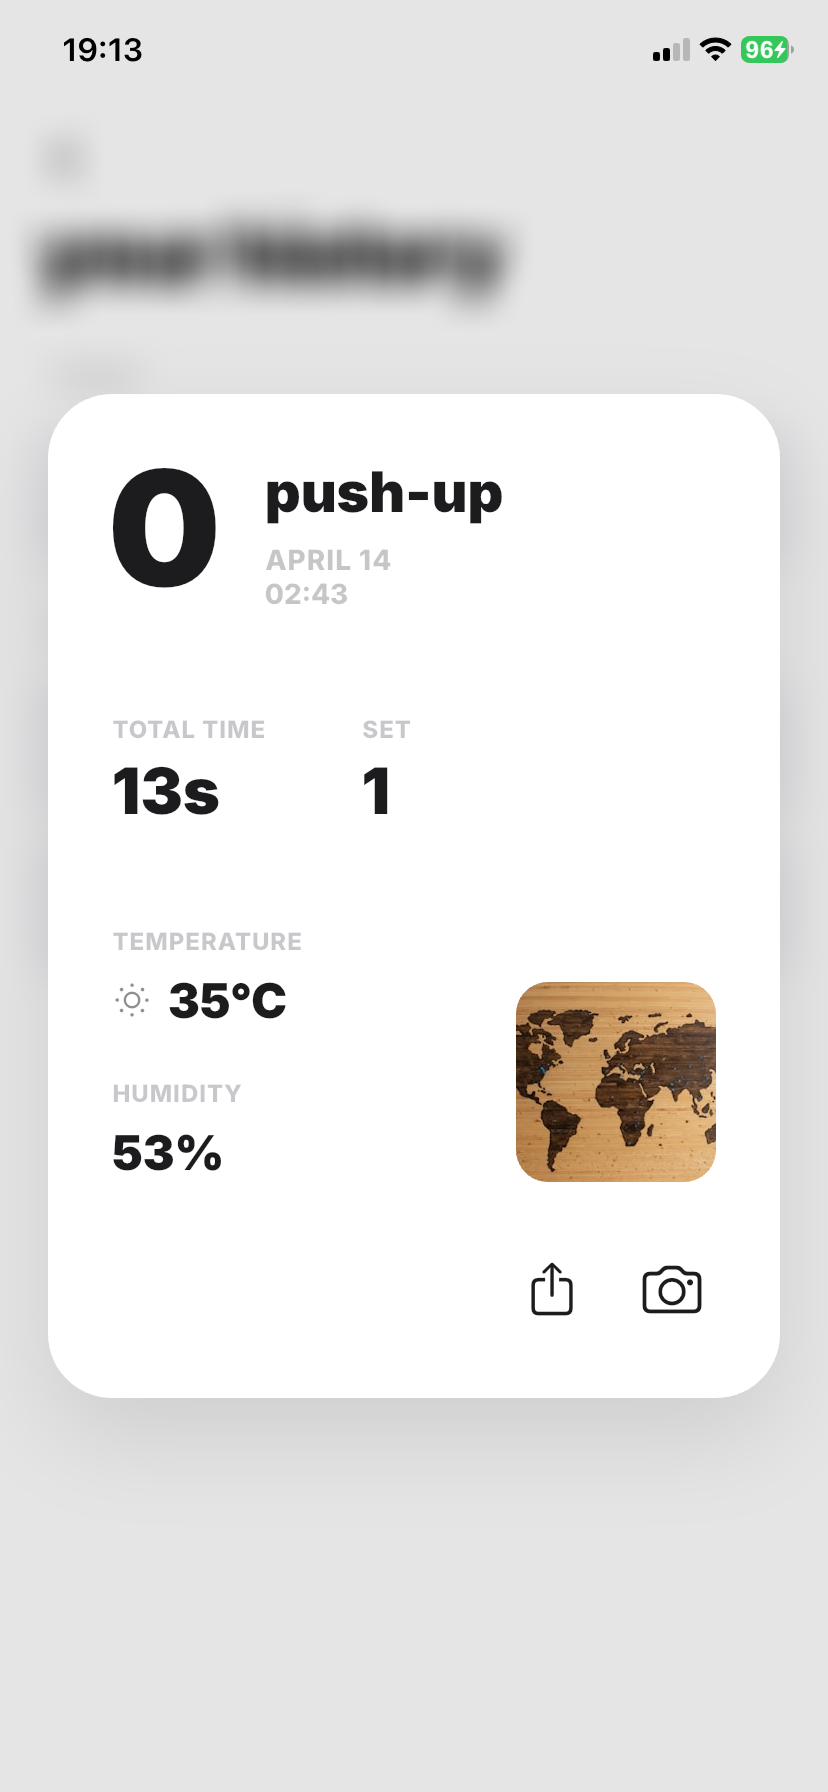
\includegraphics[height=9.5cm]{push_up/IMG_6875.PNG}
        \caption{Thẻ báo cáo chia sẻ buổi tập (Workout Report).}
        \label{fig:pushup_report}
    \end{minipage}
\end{figure}

\newpage
\begin{figure}[htbp]
    \centering
    \begin{minipage}{0.45\textwidth}
        \centering
        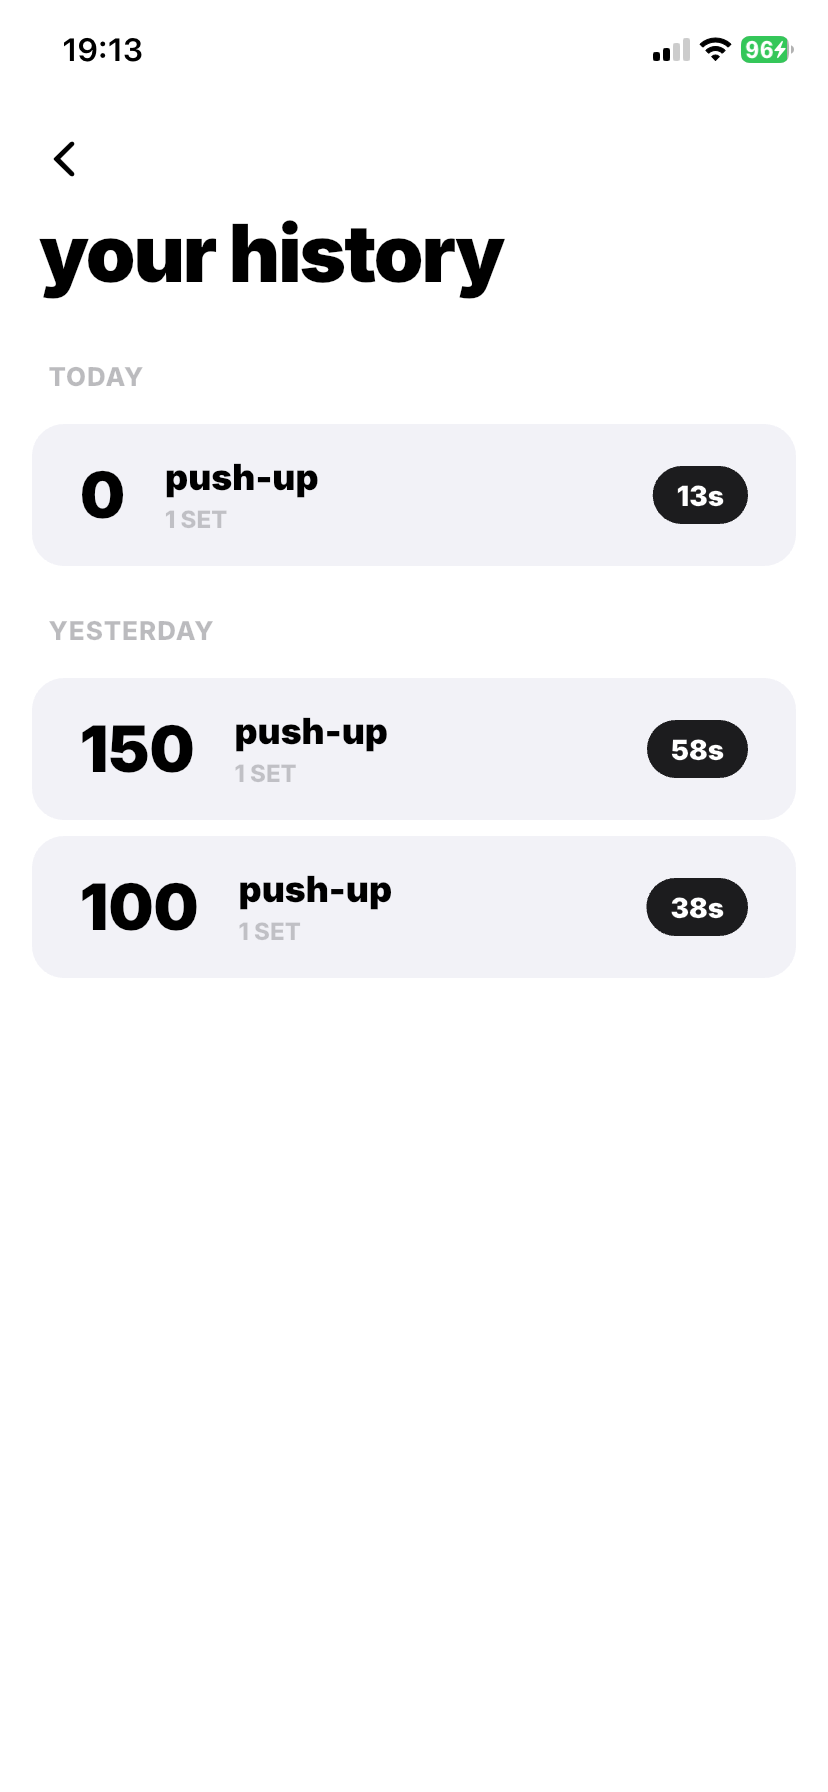
\includegraphics[height=9.5cm]{push_up/IMG_6874.PNG}
        \caption{Giao diện quản lý lịch sử các buổi tập (History).}
        \label{fig:pushup_history}
    \end{minipage}
    \hfill
    \begin{minipage}{0.45\textwidth}
        \centering
        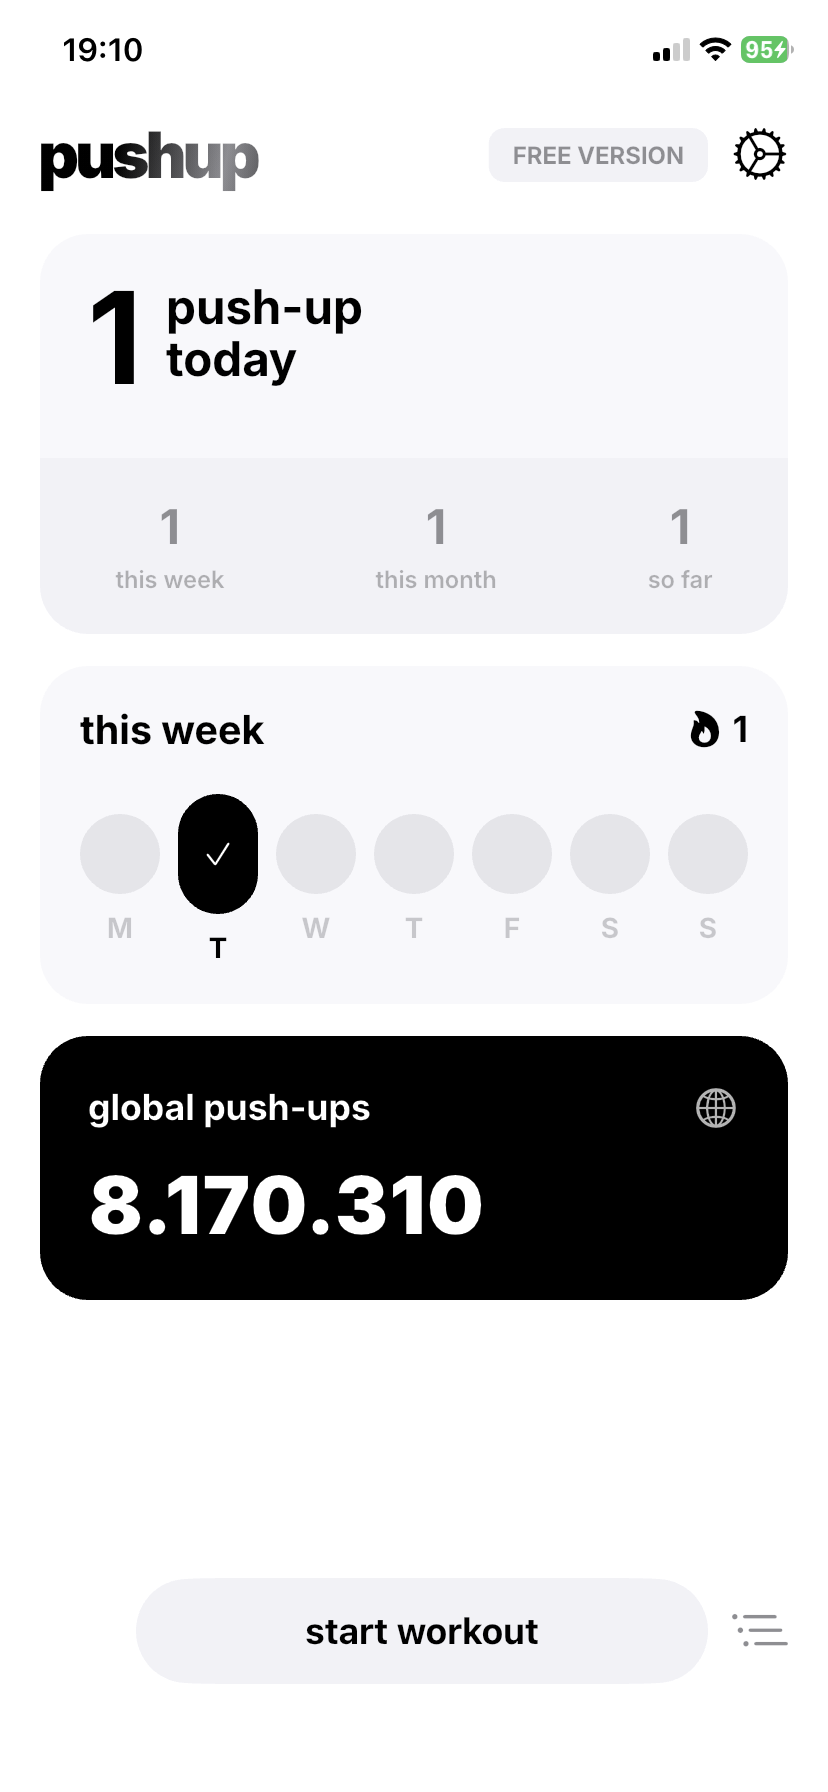
\includegraphics[height=9.5cm]{push_up/IMG_6873.PNG}
        \caption{Dashboard ghi nhận hít đất thành công đầu tiên.}
        \label{fig:pushup_success}
    \end{minipage}
\end{figure}

\newpage
\subsection*{Phần 3: Dự án PDF Converter \& Scanner (Giai đoạn 3)}
Ứng dụng quét tài liệu chuyên nghiệp và chuyển đổi đa định dạng ngoại tuyến:

\subsubsection*{3.1. Màn hình Convert và luồng nhập liệu đa nguồn}
\begin{figure}[htbp]
    \centering
    \begin{minipage}{0.45\textwidth}
        \centering
        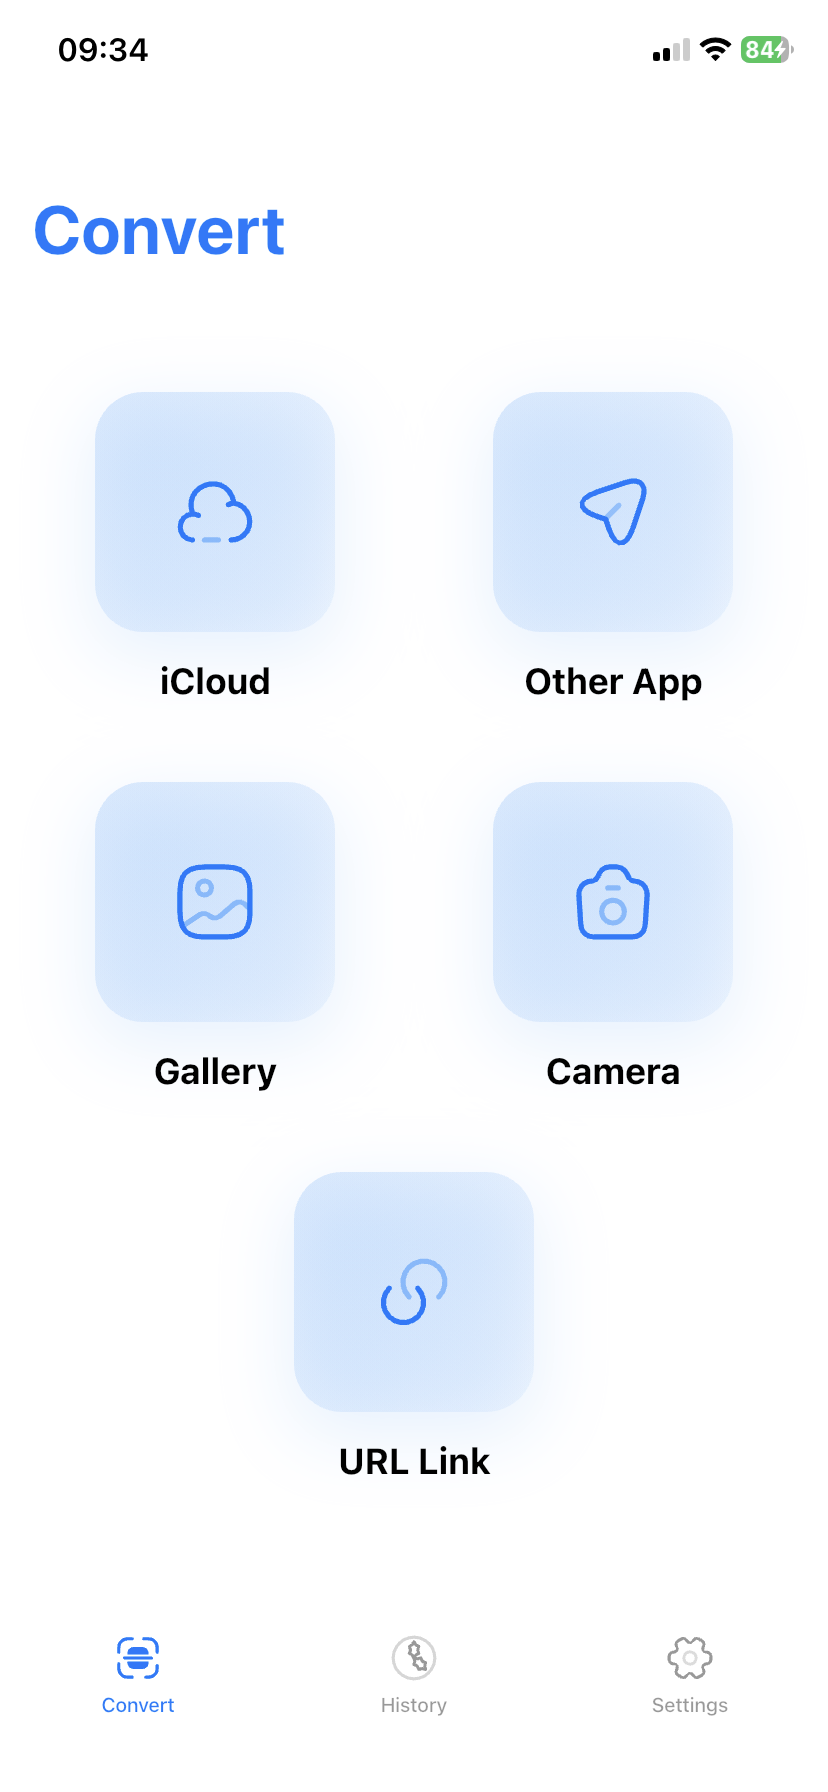
\includegraphics[height=9.5cm]{features/IMG_7576.PNG}
        \caption{Màn hình Convert chính với 5 nguồn nhập liệu: iCloud, Other App, Gallery, Camera, URL Link.}
        \label{fig:pdf_convert_home}
    \end{minipage}
    \hfill
    \begin{minipage}{0.45\textwidth}
        \centering
        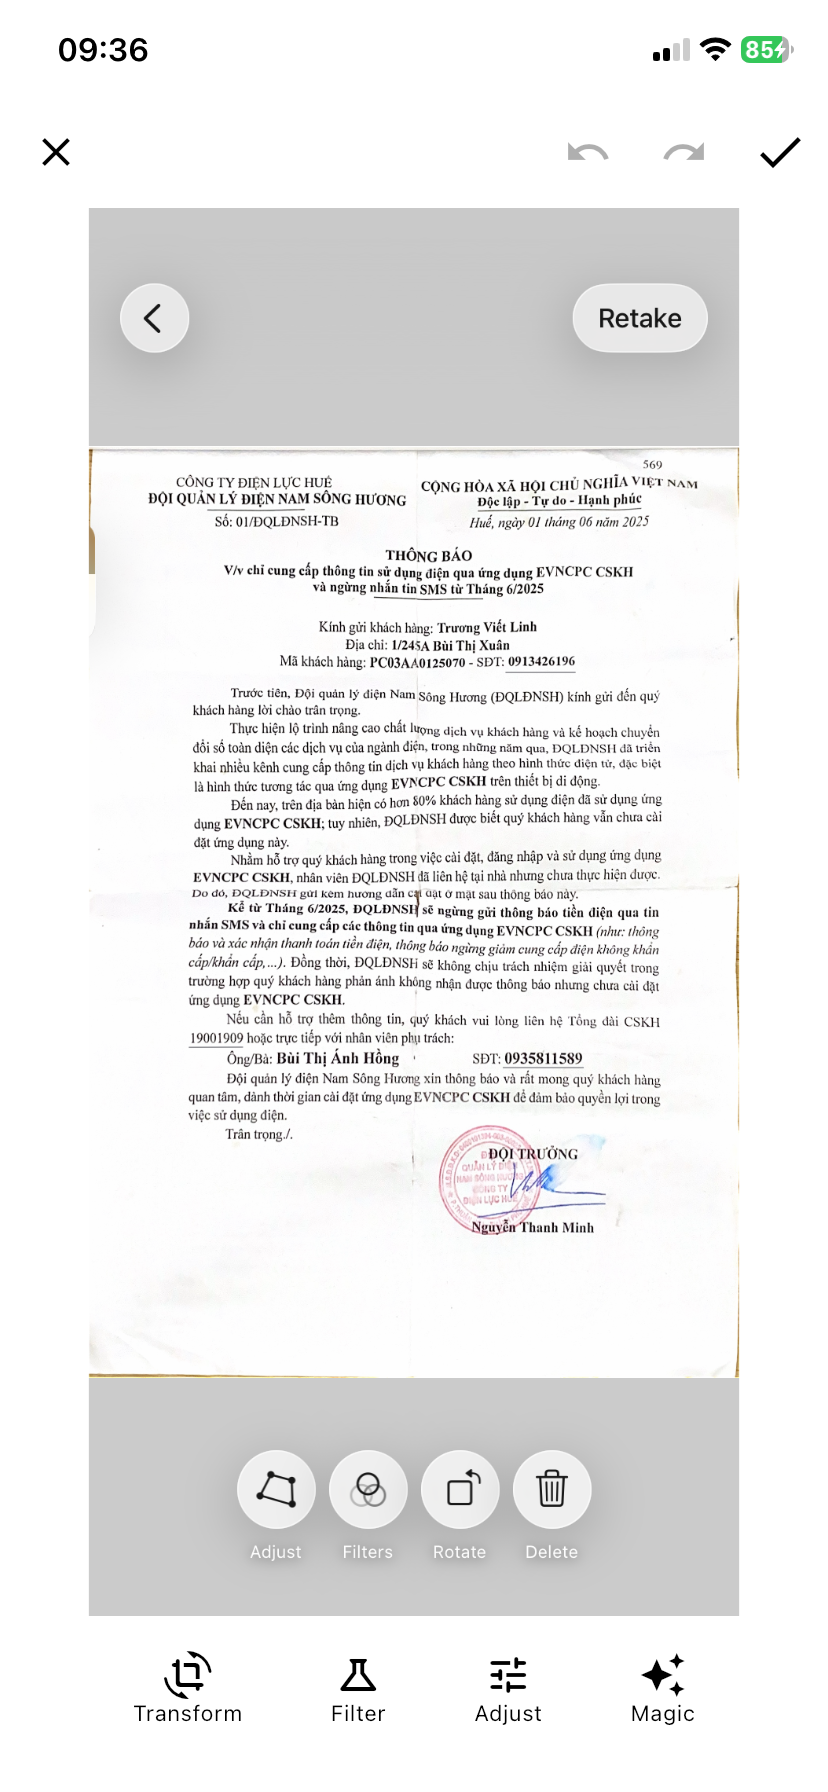
\includegraphics[height=9.5cm]{features/IMG_7592.PNG}
        \caption{Popup ``Enter URL'': nhập liên kết URL để tải và chuyển đổi tài liệu trực tiếp từ Internet.}
        \label{fig:pdf_url}
    \end{minipage}
\end{figure}

\begin{figure}[htbp]
    \centering
    \begin{minipage}{0.45\textwidth}
        \centering
        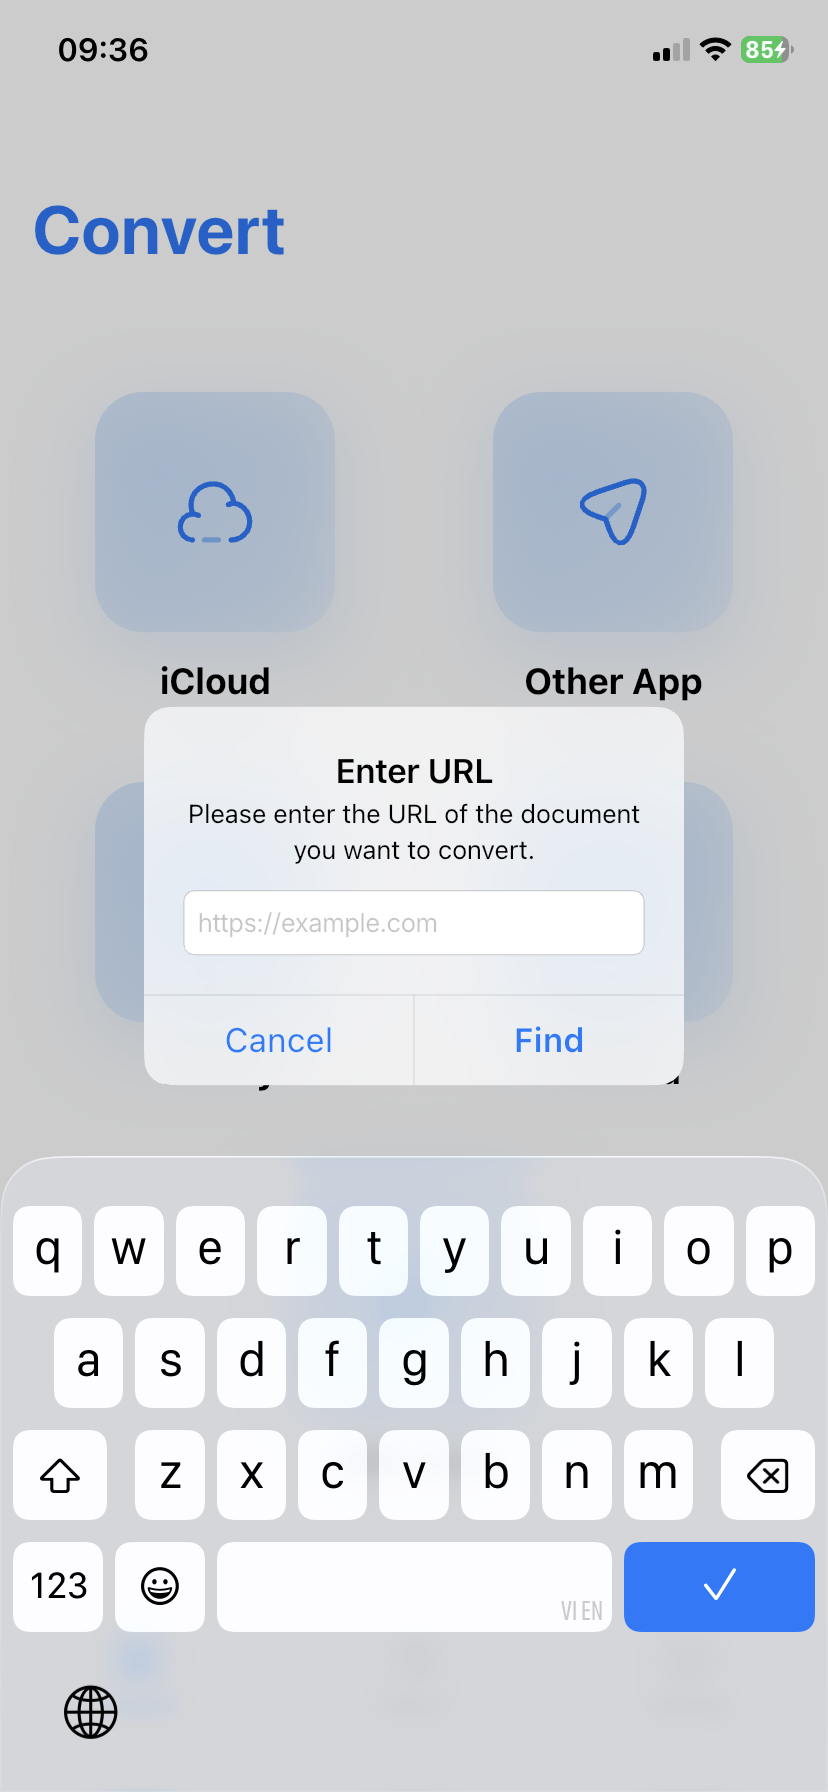
\includegraphics[height=9.5cm]{features/IMG_7593.PNG}
        \caption{Màn hình iCloud Picker: chọn file từ iCloud Drive (Gần đây, Được chia sẻ, Duyệt) với thanh tìm kiếm.}
        \label{fig:pdf_icloud}
    \end{minipage}
    \hfill
    \begin{minipage}{0.45\textwidth}
        \centering
        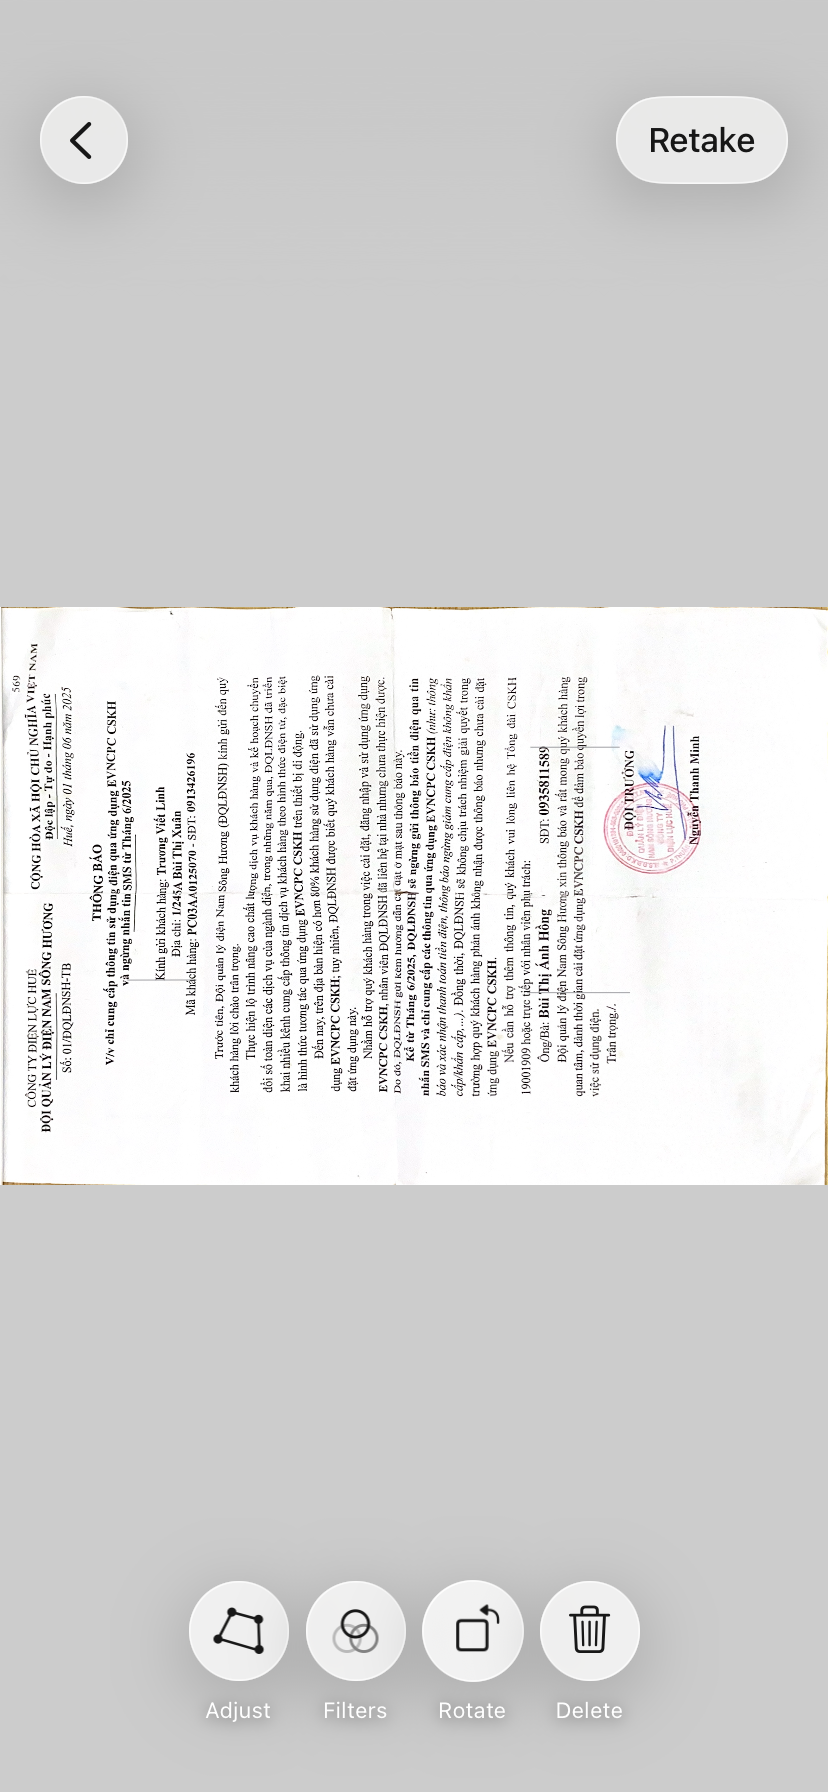
\includegraphics[height=9.5cm]{features/IMG_7584.PNG}
        \caption{Màn hình New Conversion: file đã chọn, định dạng đích .pdf, PDF Settings chất lượng 90\%, nút Convert.}
        \label{fig:pdf_new_conversion}
    \end{minipage}
\end{figure}

\newpage
\subsubsection*{3.2. Quét tài liệu qua Camera và hiệu chỉnh phối cảnh}
\begin{figure}[htbp]
    \centering
    \begin{minipage}{0.45\textwidth}
        \centering
        \includegraphics[height=9.5cm]{features/IMG_7580.PNG}
        \caption{Giao diện Camera Scanner: quét tài liệu trực tiếp với thanh điều khiển Flash, Filters, Shutter.}
        \label{fig:pdf_camera}
    \end{minipage}
    \hfill
    \begin{minipage}{0.45\textwidth}
        \centering
        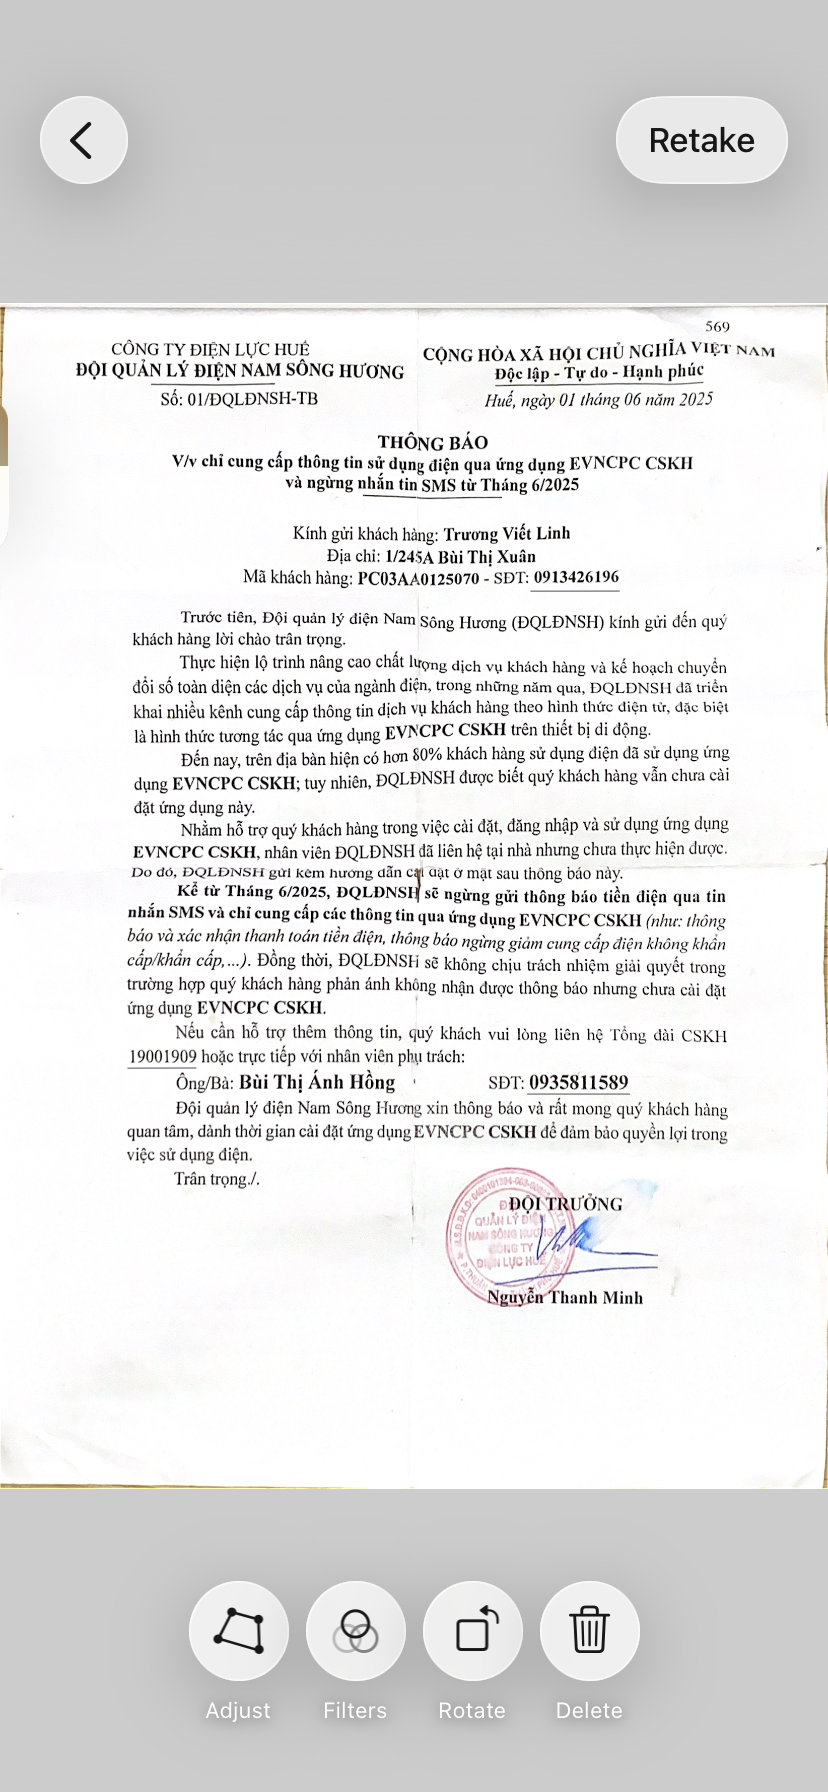
\includegraphics[height=9.5cm]{features/IMG_7581.PNG}
        \caption{Màn hình Perspective Crop: hiệu chỉnh phối cảnh tài liệu với 4 đỉnh tương tác và toolbar Adjust/Filters/Rotate/Delete.}
        \label{fig:pdf_crop}
    \end{minipage}
\end{figure}

\begin{figure}[htbp]
    \centering
    \begin{minipage}{0.45\textwidth}
        \centering
        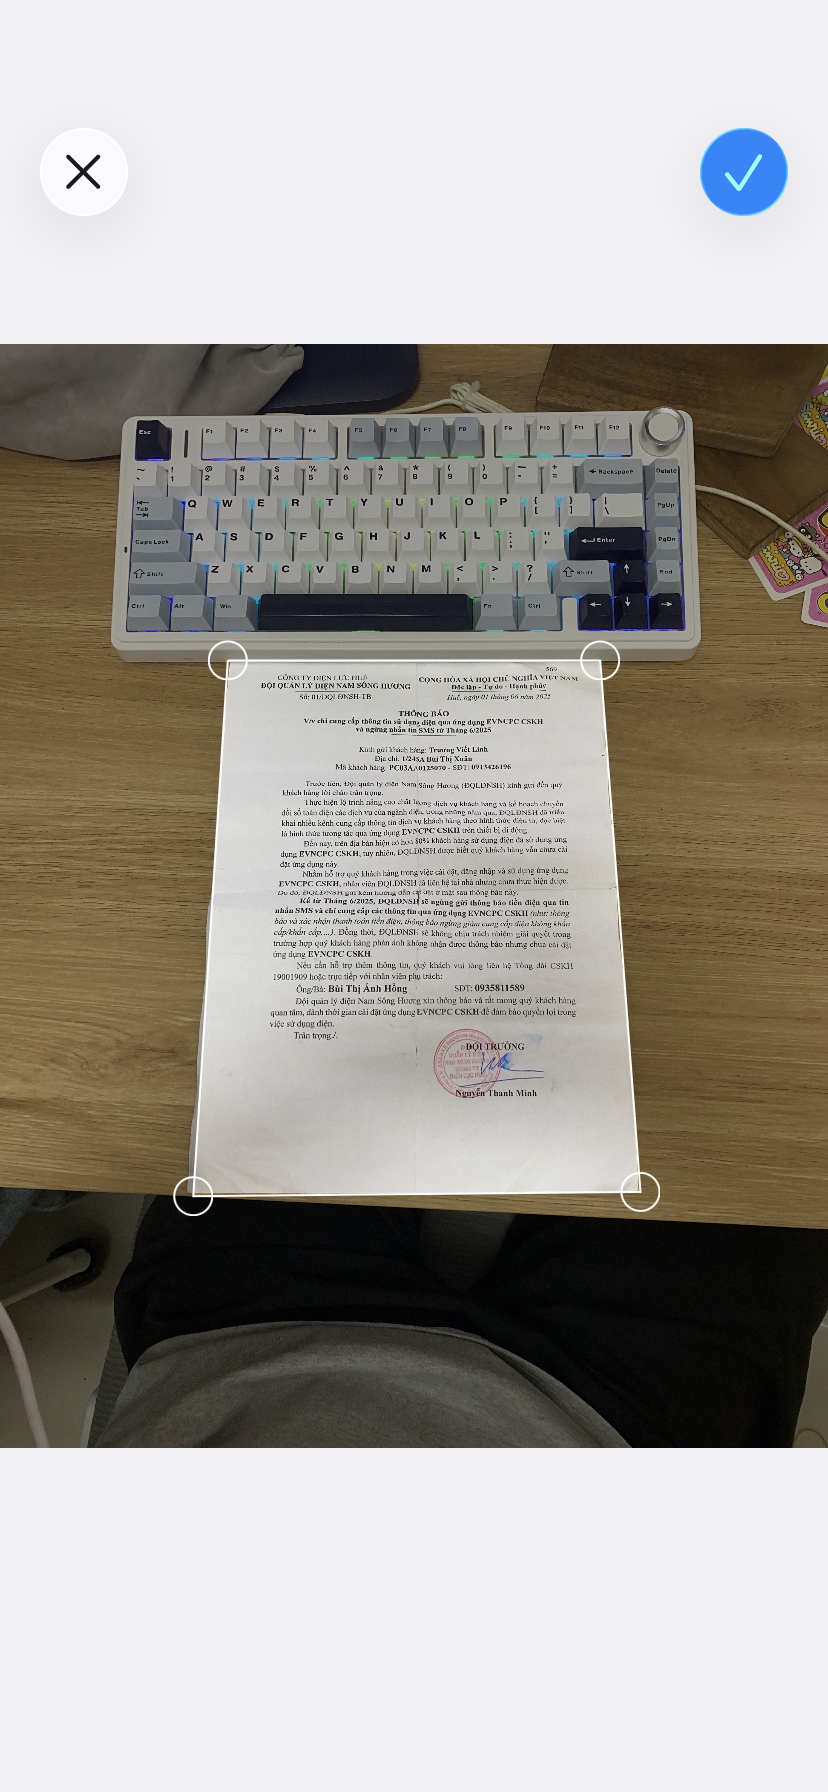
\includegraphics[height=9.5cm]{features/IMG_7582.PNG}
        \caption{Picker chọn bộ lọc tài liệu: Black \& White, Grayscale, Color, Photo để chuẩn hóa ảnh quét.}
        \label{fig:pdf_filter_picker}
    \end{minipage}
    \hfill
    \begin{minipage}{0.45\textwidth}
        \centering
        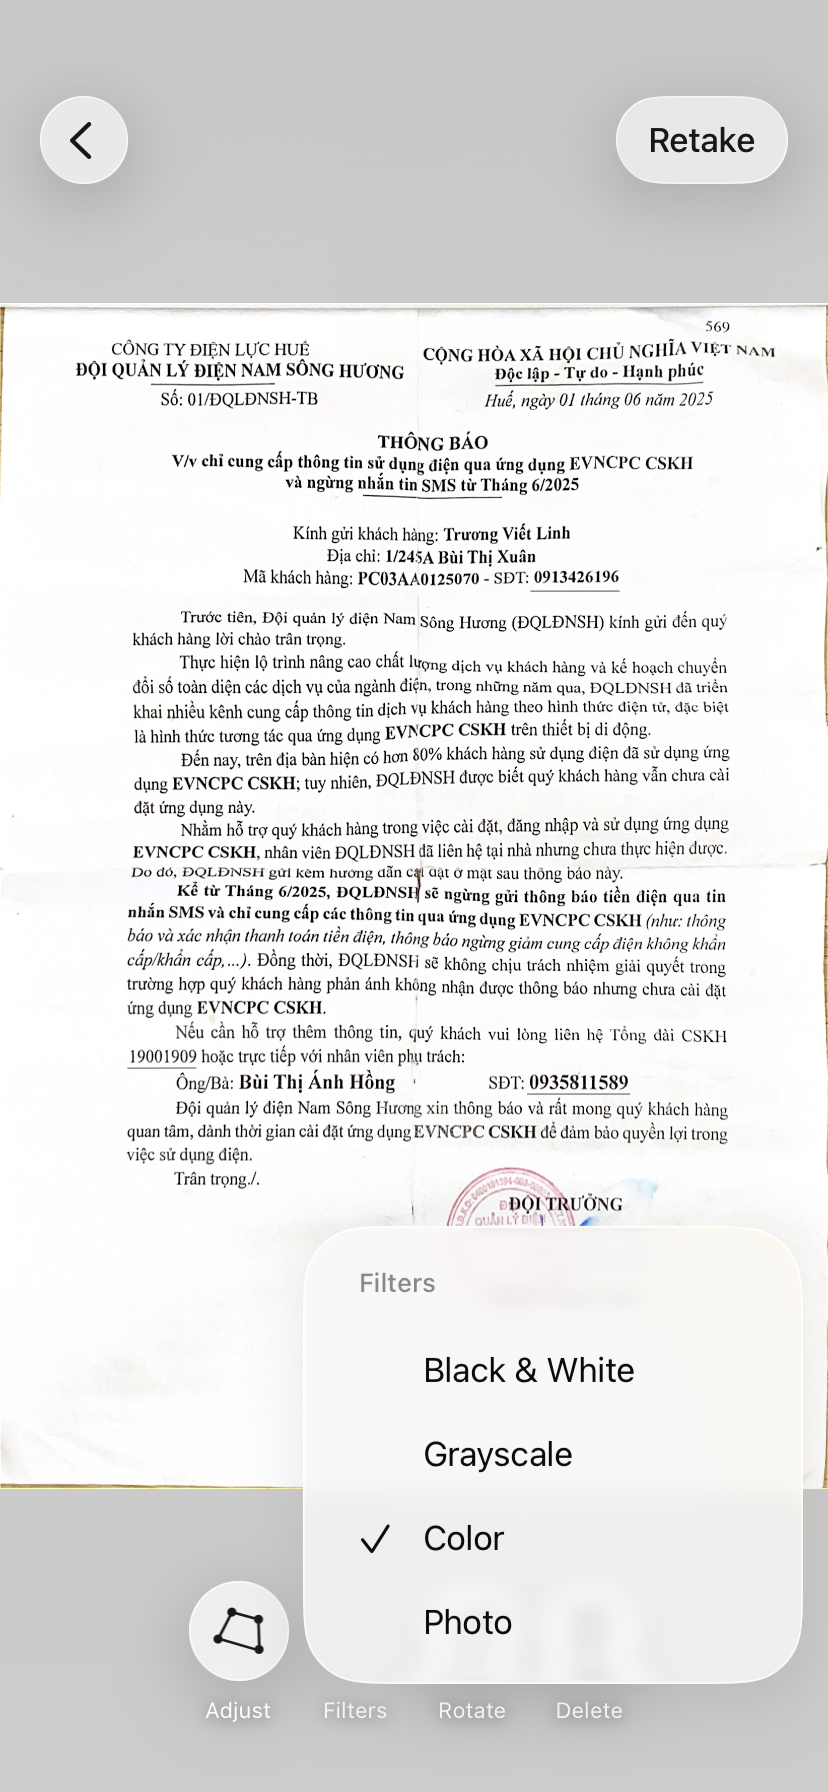
\includegraphics[height=9.5cm]{features/IMG_7583.PNG}
        \caption{Kết quả sau khi xoay tài liệu quét sang chế độ ngang (Rotate), sẵn sàng xác nhận lưu.}
        \label{fig:pdf_rotated}
    \end{minipage}
\end{figure}

\newpage
\subsubsection*{3.3. Bộ chỉnh sửa ảnh nâng cao và chọn định dạng đích}
\begin{figure}[htbp]
    \centering
    \begin{minipage}{0.45\textwidth}
        \centering
        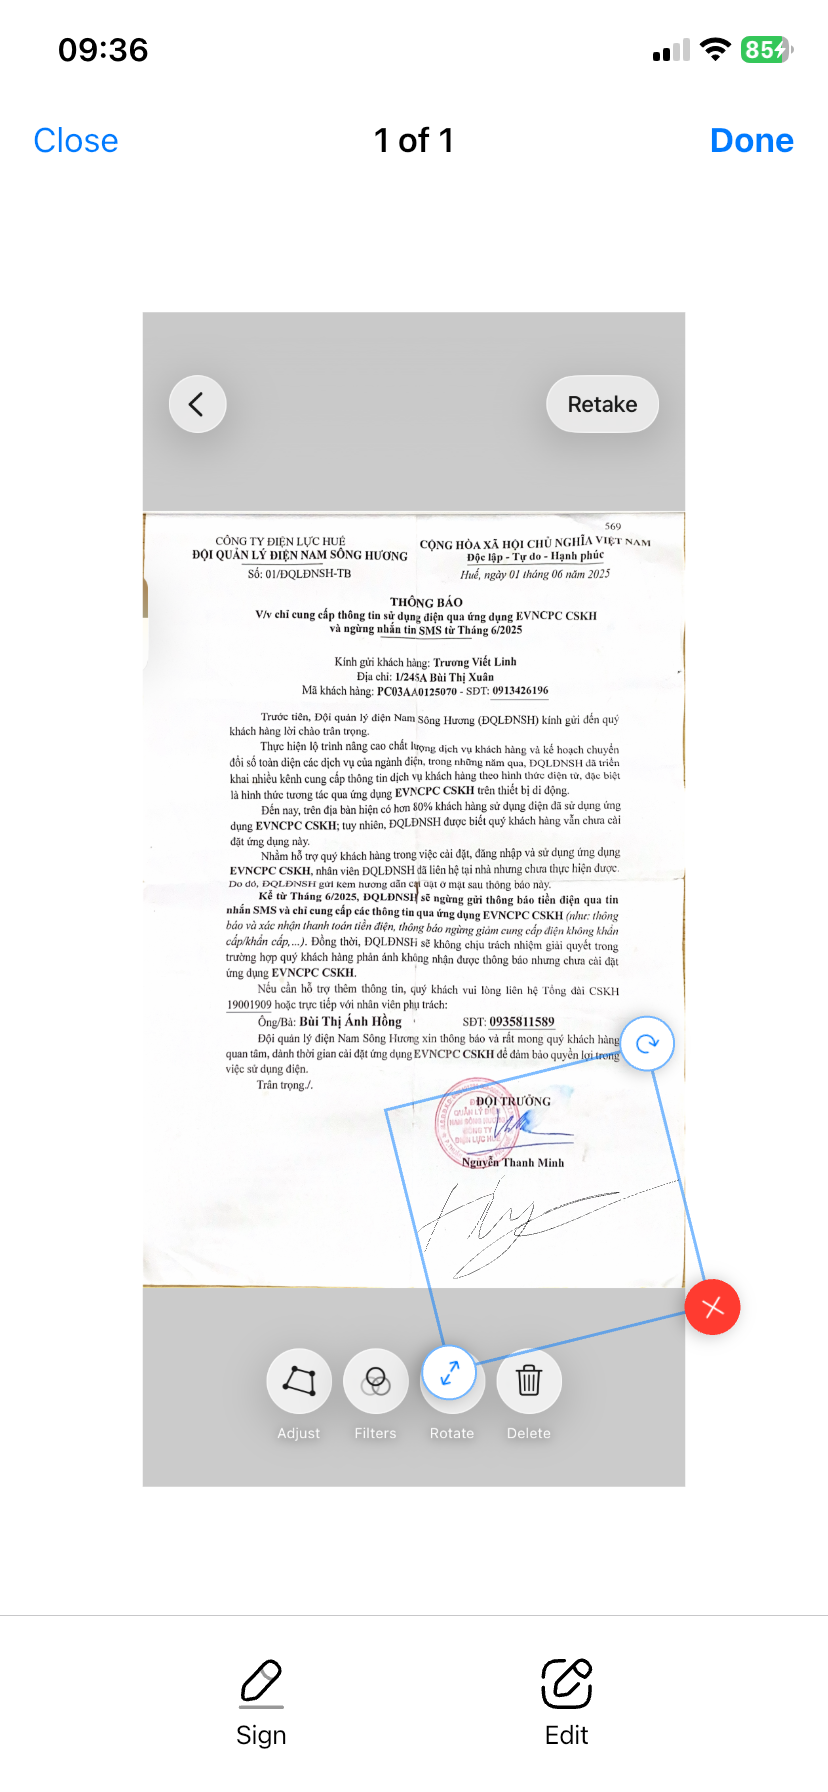
\includegraphics[height=9.5cm]{features/IMG_7591.PNG}
        \caption{Bộ pro\_image\_editor tích hợp sâu với 4 công cụ chỉnh sửa: Transform, Filter, Adjust, Magic.}
        \label{fig:pdf_pro_editor}
    \end{minipage}
    \hfill
    \begin{minipage}{0.45\textwidth}
        \centering
        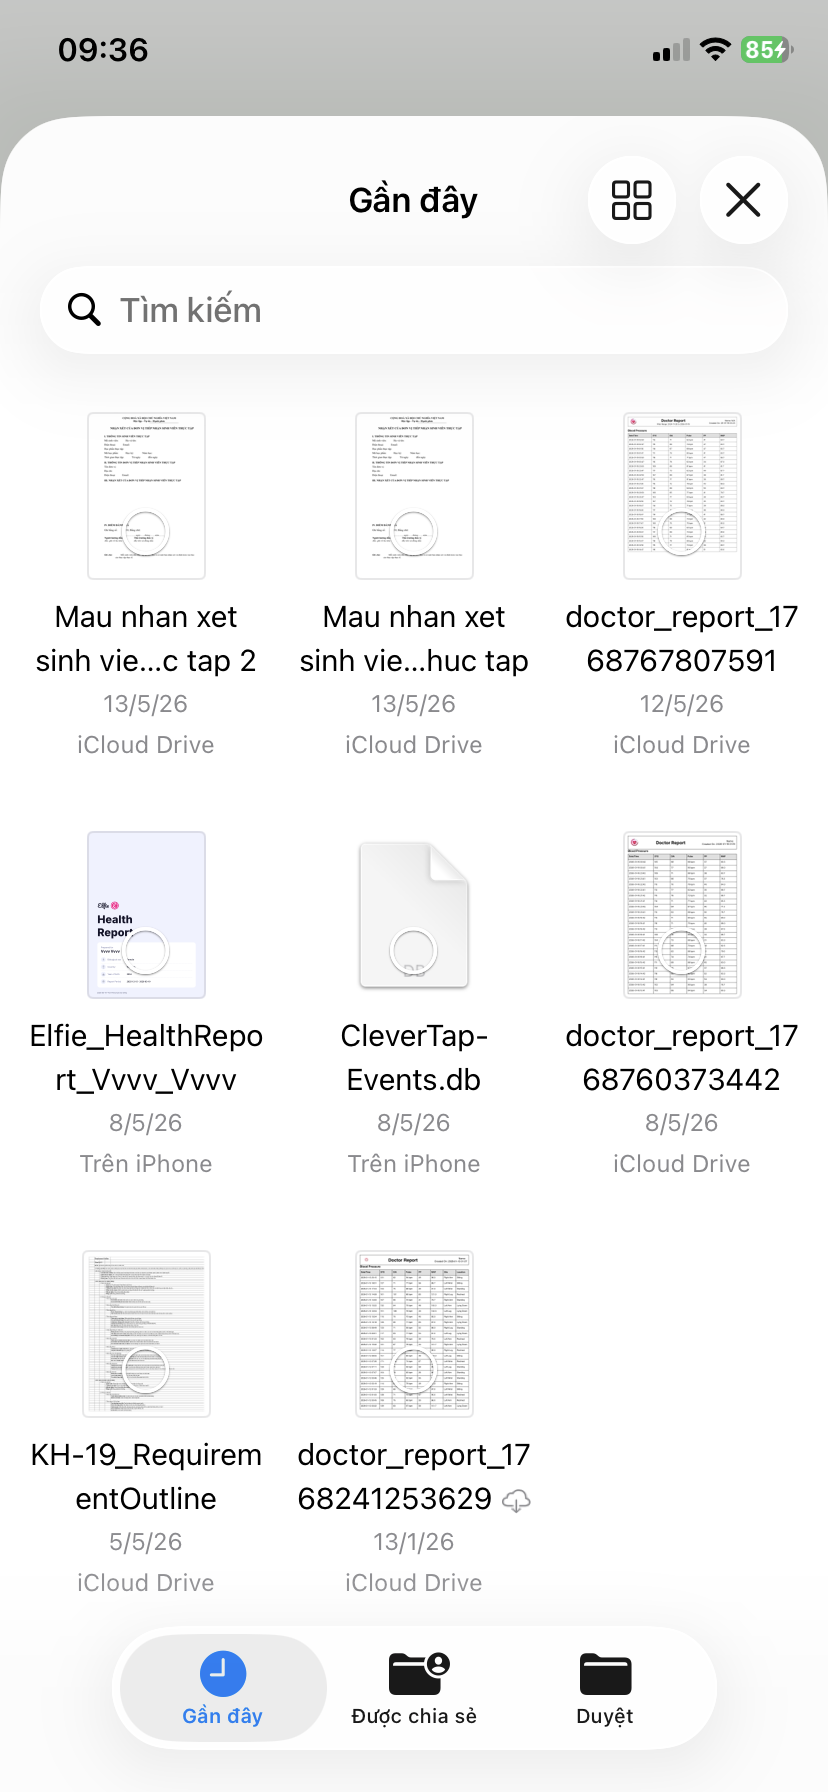
\includegraphics[height=9.5cm]{features/IMG_7594.PNG}
        \caption{Màn hình Target extension: chọn định dạng đích .pdf, .doc, .docx, .jpg, .png, .epub, .txt, .xls, .xlsx, .mobi, .ppt.}
        \label{fig:pdf_target_ext}
    \end{minipage}
\end{figure}

\begin{figure}[htbp]
    \centering
    \begin{minipage}{0.45\textwidth}
        \centering
        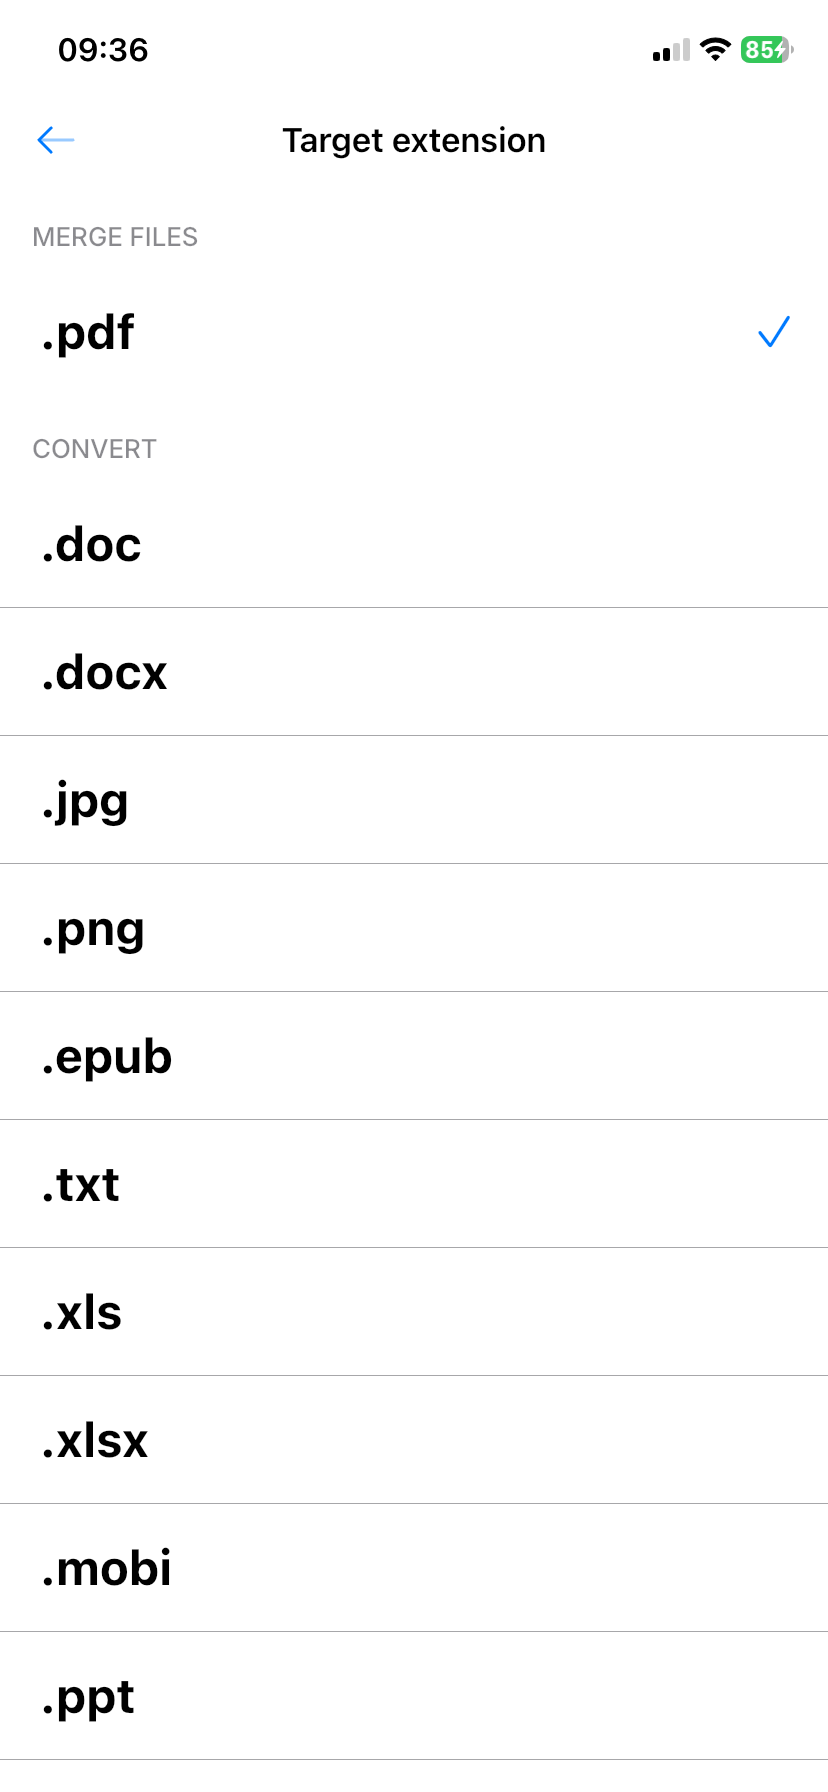
\includegraphics[height=9.5cm]{features/IMG_7595.PNG}
        \caption{Màn hình Target extension đầy đủ: nhóm Merge Files (.pdf) và toàn bộ định dạng Convert đa dạng.}
        \label{fig:pdf_formats_full}
    \end{minipage}
    \hfill
    \begin{minipage}{0.45\textwidth}
        \centering
        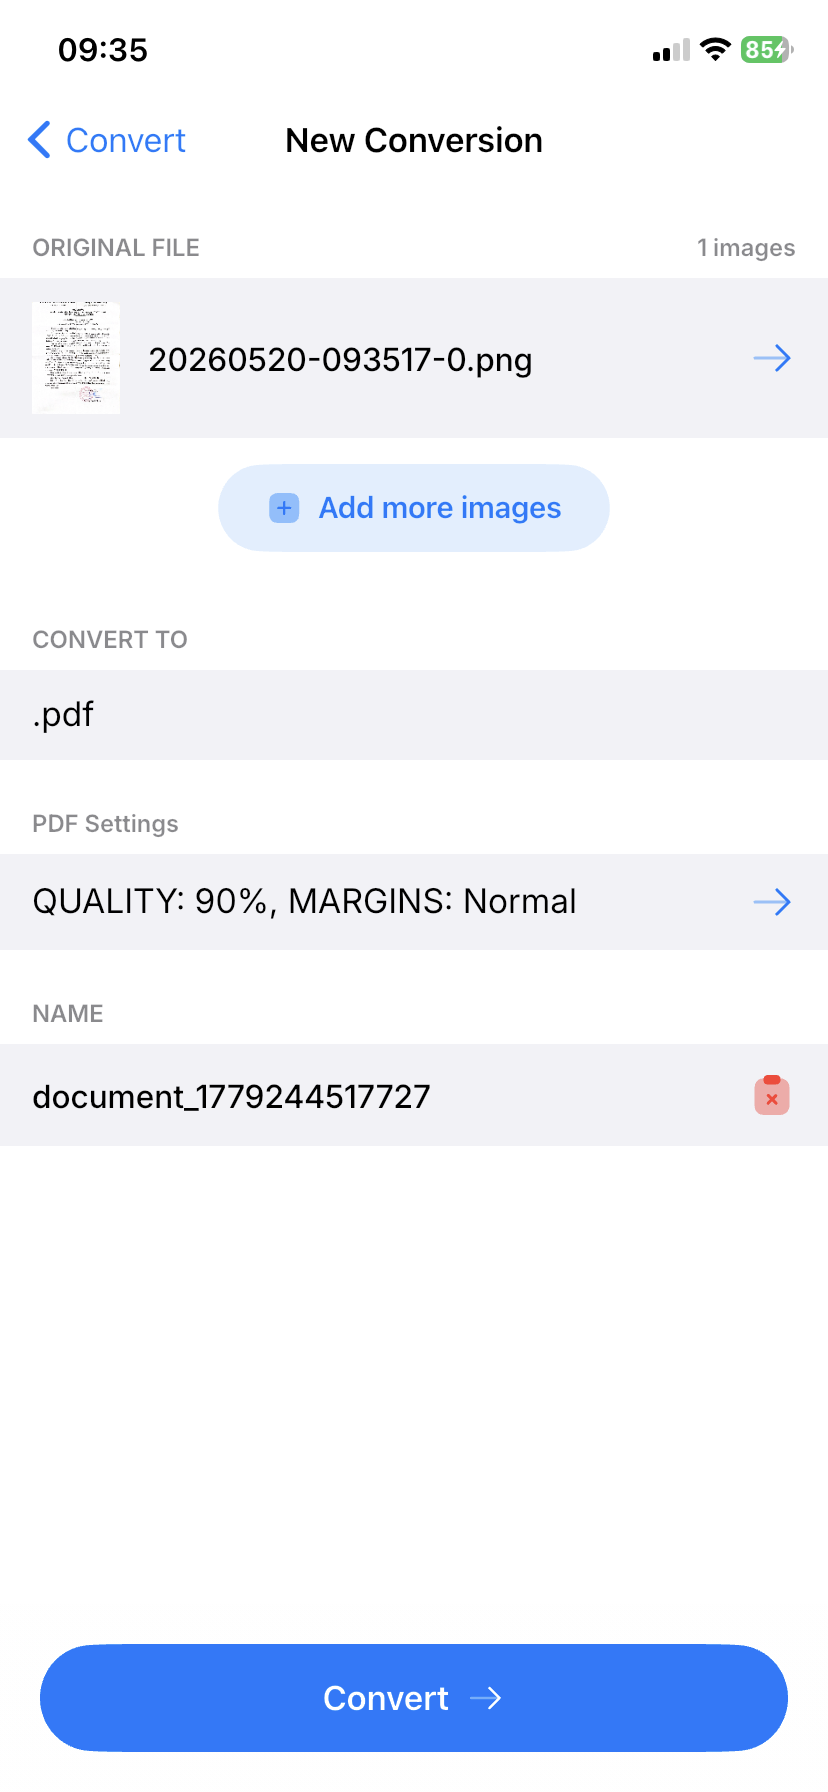
\includegraphics[height=9.5cm]{features/IMG_7585.PNG}
        \caption{Màn hình ``Creating PDF'': Circular Progress Indicator hiển thị 6\% với thông điệp ``Optimizing PDF...''}
        \label{fig:pdf_progress}
    \end{minipage}
\end{figure}

\newpage
\subsubsection*{3.4. Xuất tệp PDF và xem trước tài liệu}
\begin{figure}[htbp]
    \centering
    \begin{minipage}{0.45\textwidth}
        \centering
        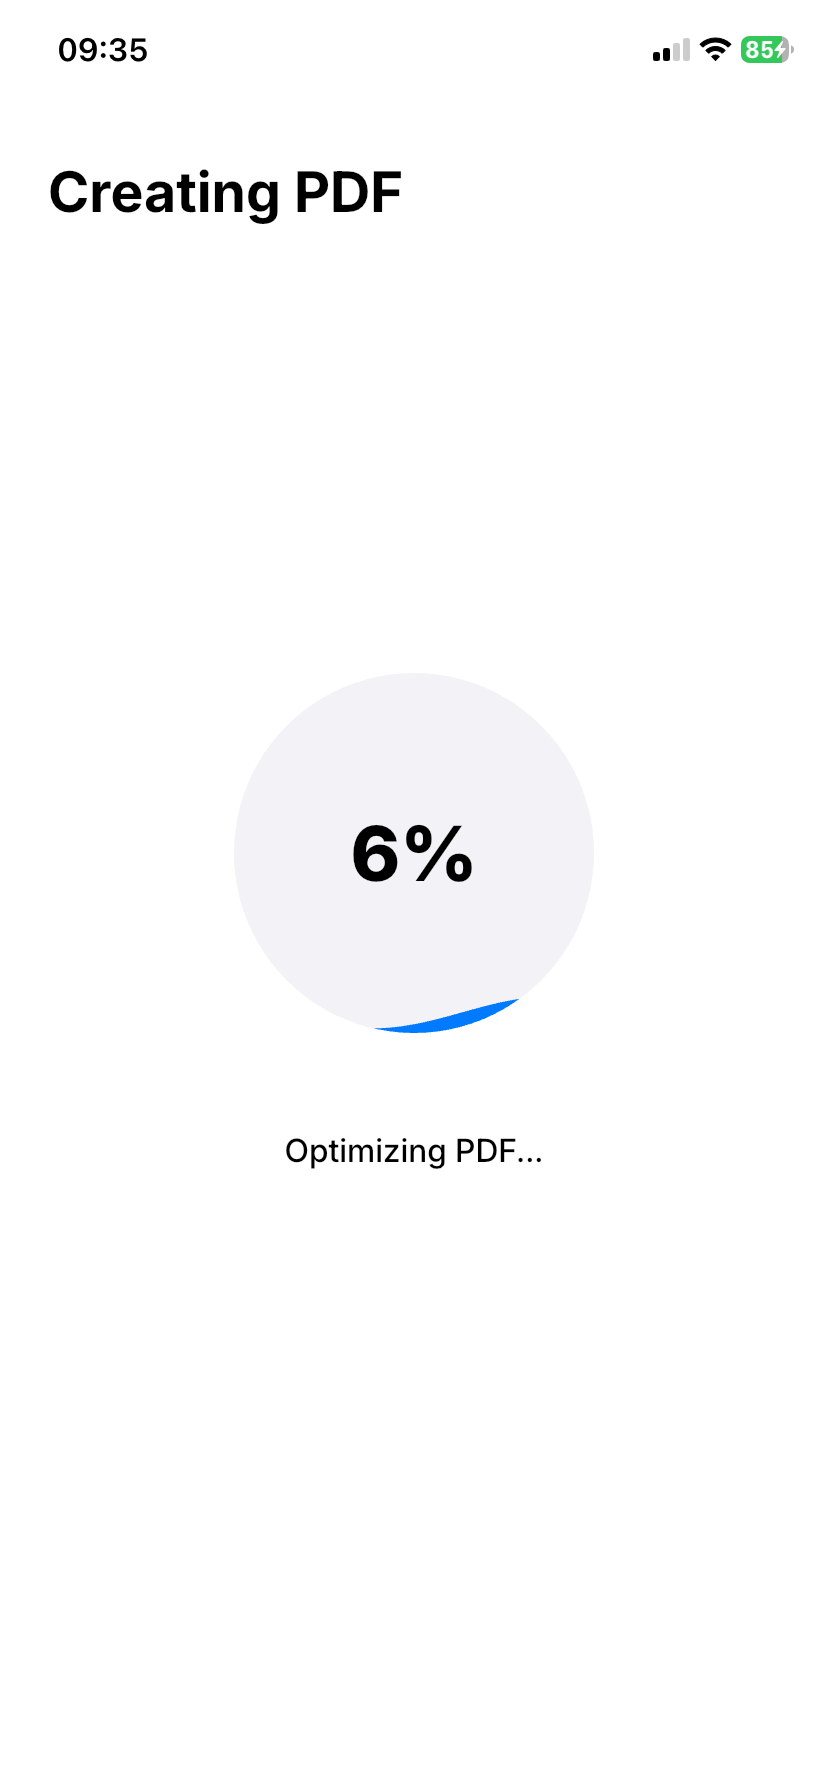
\includegraphics[height=9.5cm]{features/IMG_7586.PNG}
        \caption{Màn hình ``PDF Exported Successfully'' và iOS Share Sheet: chia sẻ qua AirDrop, Mail, Zalo và ứng dụng khác.}
        \label{fig:pdf_exported}
    \end{minipage}
    \hfill
    \begin{minipage}{0.45\textwidth}
        \centering
        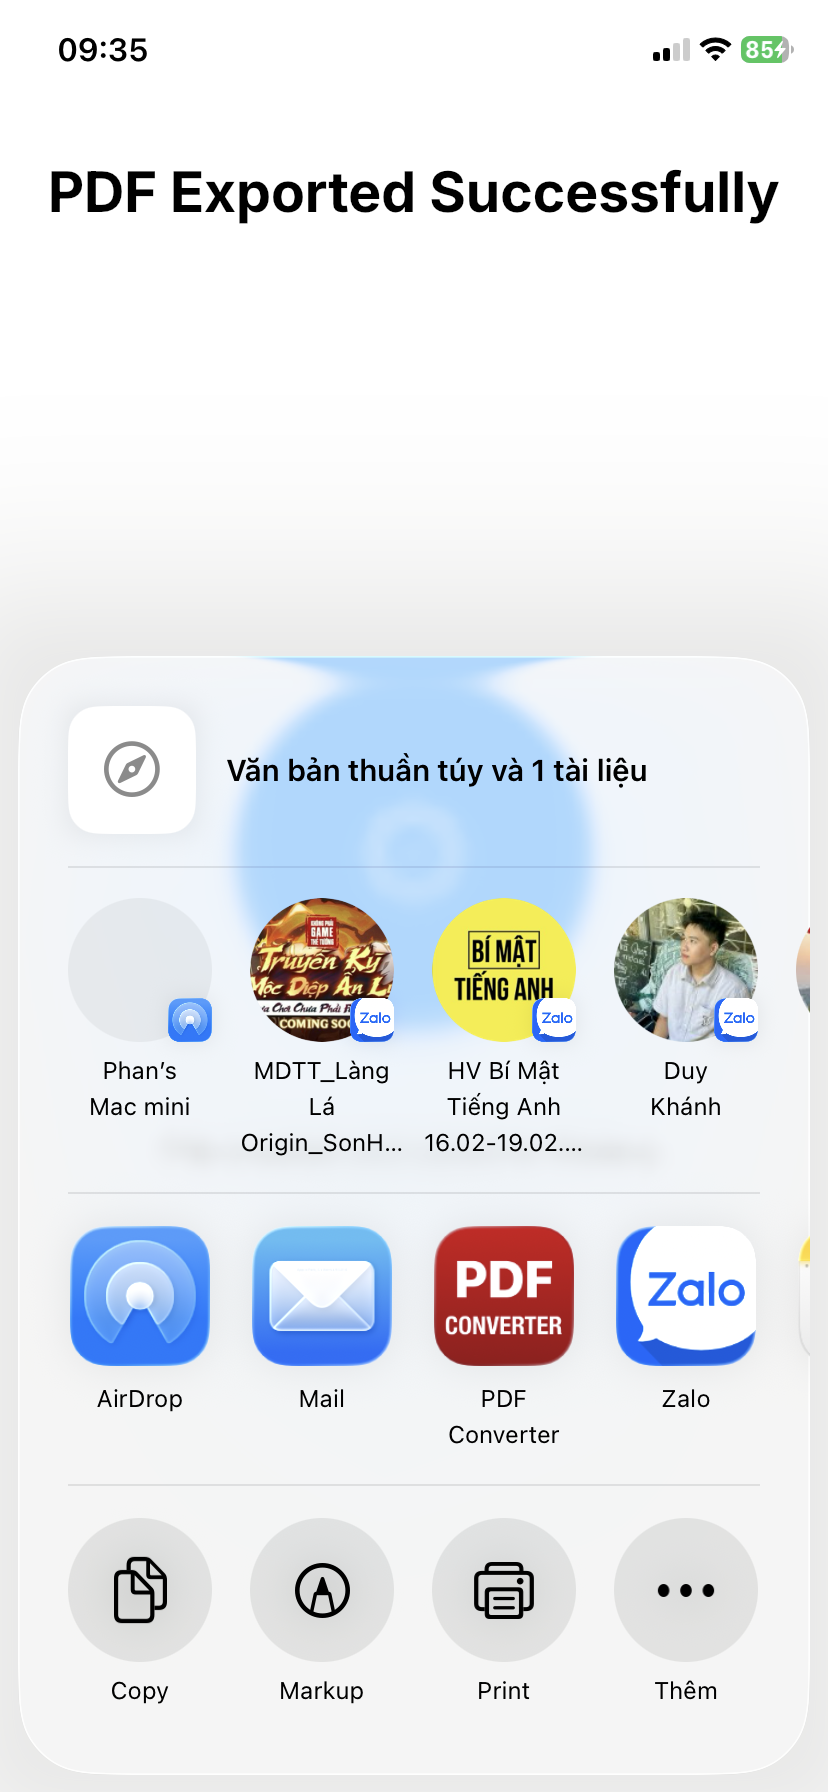
\includegraphics[height=9.5cm]{features/IMG_7587.PNG}
        \caption{Màn hình xem trước PDF sau chuyển đổi (1 of 1) với nút Sign (Ký chữ ký) và Edit (Chỉnh sửa ảnh).}
        \label{fig:pdf_preview}
    \end{minipage}
\end{figure}

\newpage
\subsubsection*{3.5. Phân hệ Chữ ký tay số (Digital Signature)}
\begin{figure}[htbp]
    \centering
    \begin{minipage}{0.45\textwidth}
        \centering
        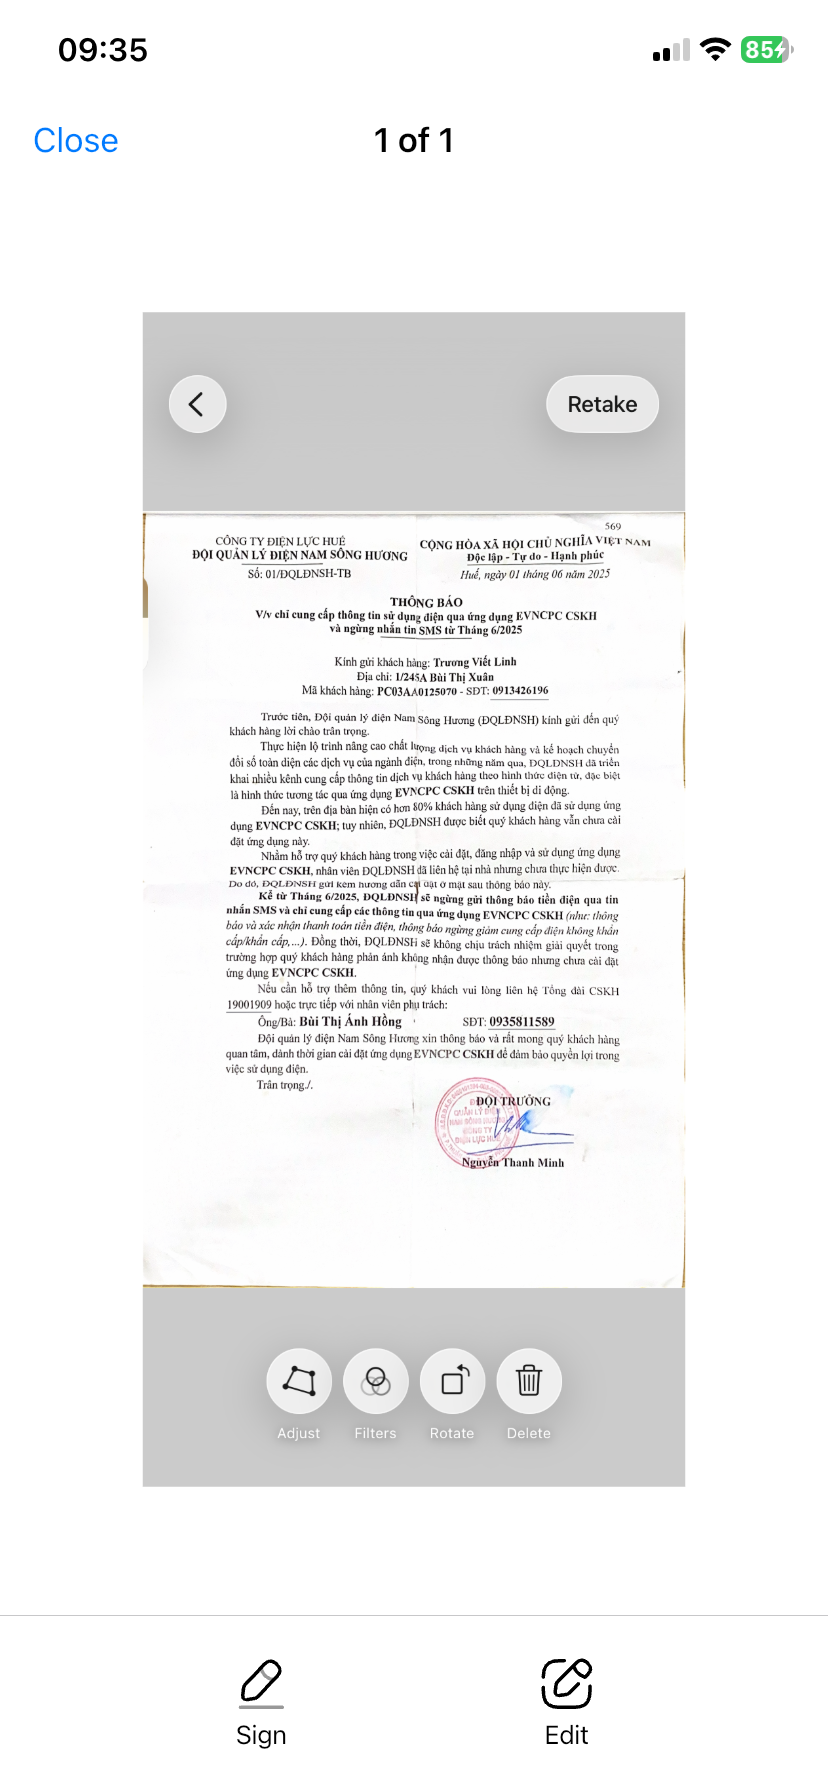
\includegraphics[height=9.5cm]{features/IMG_7588.PNG}
        \caption{Màn hình ``Choose signature'': tạo New signature hoặc chọn lại chữ ký đã lưu (Saved 1, Saved 2).}
        \label{fig:pdf_choose_sig}
    \end{minipage}
    \hfill
    \begin{minipage}{0.45\textwidth}
        \centering
        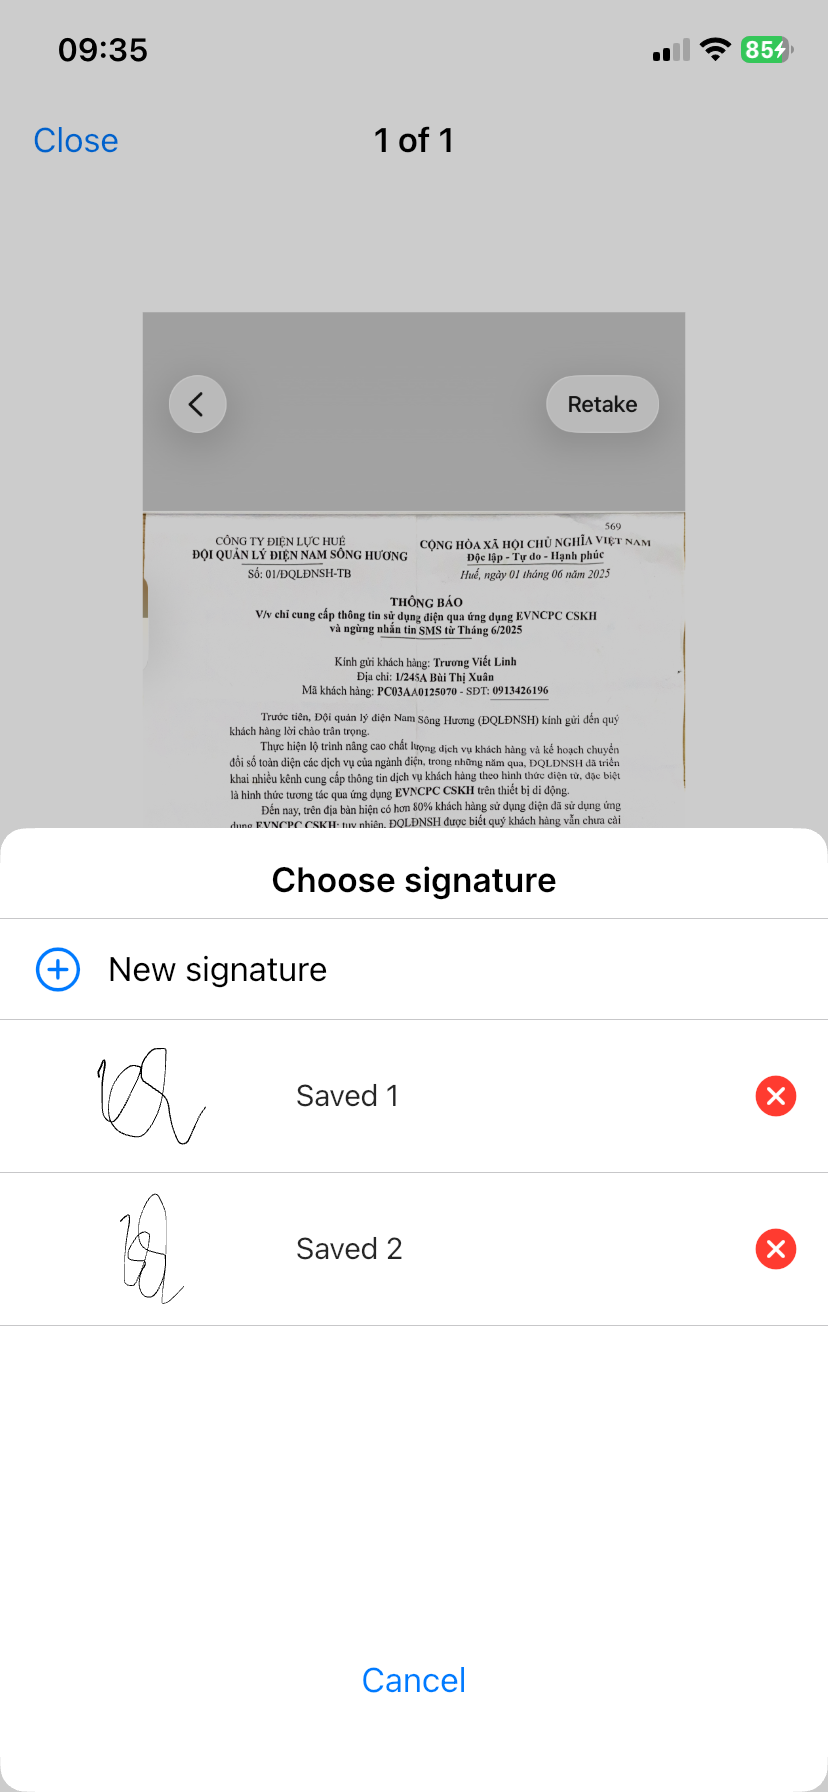
\includegraphics[height=9.5cm]{features/IMG_7589.PNG}
        \caption{Canvas vẽ chữ ký tay (Draw Signature) chế độ ngang với bộ chọn màu mực (Đỏ/Xanh/Đen) và slider độ dày nét.}
        \label{fig:pdf_draw_sig}
    \end{minipage}
\end{figure}

\begin{figure}[htbp]
    \centering
    \begin{minipage}{0.45\textwidth}
        \centering
        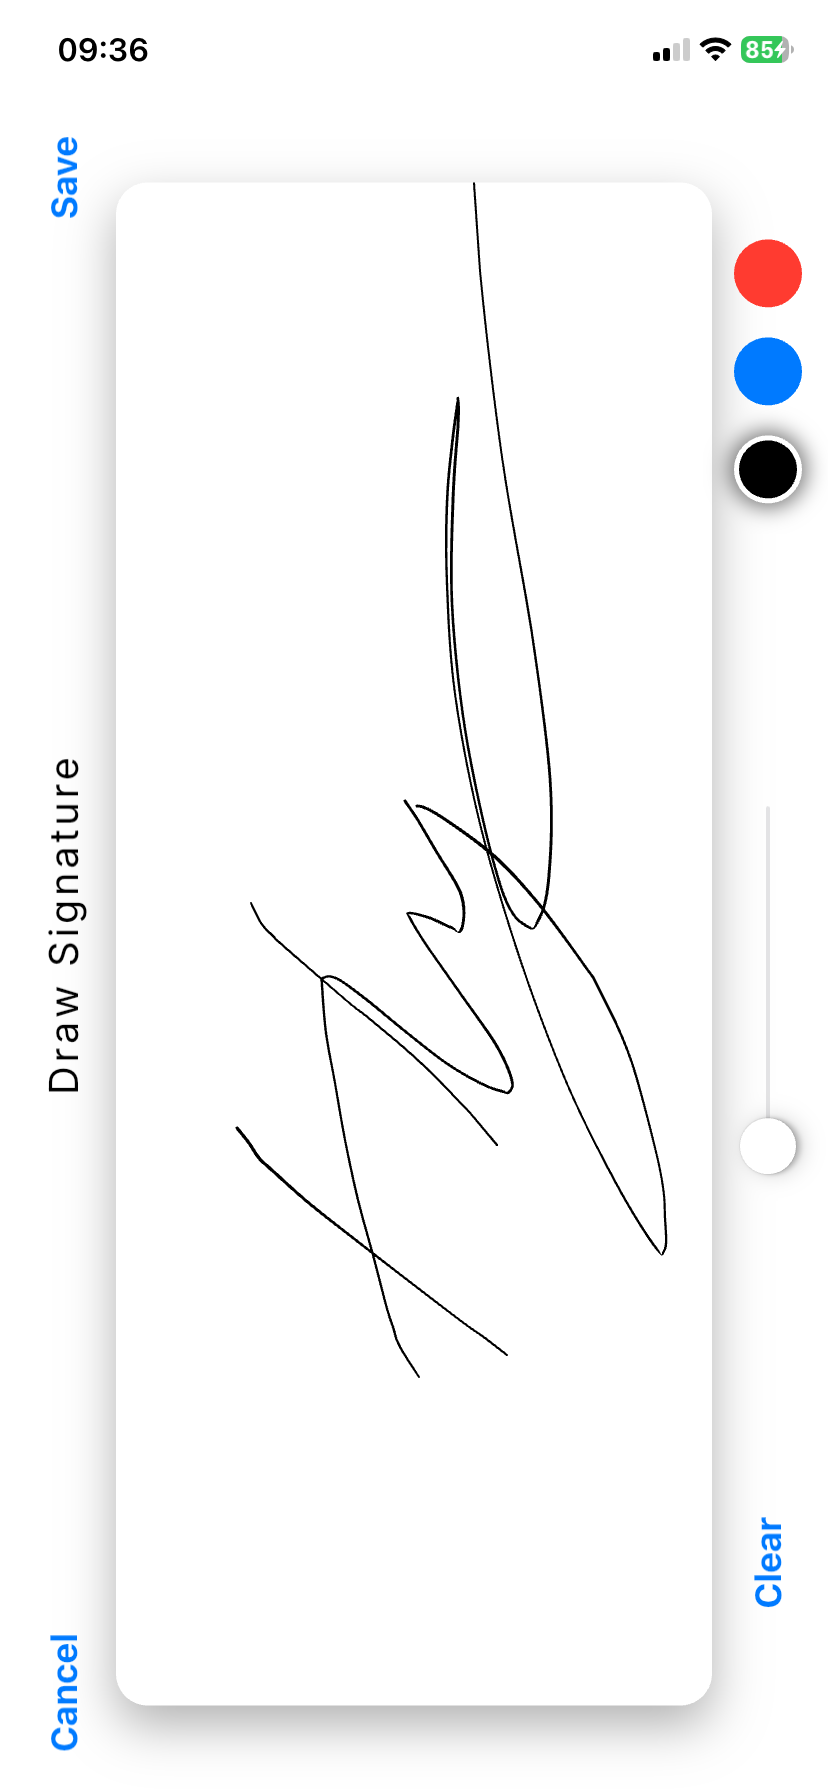
\includegraphics[height=9.5cm]{features/IMG_7590.PNG}
        \caption{Đặt chữ ký tay số lên trang PDF: tương tác kéo thả, xoay tự do, xóa bằng nút đỏ trực quan.}
        \label{fig:pdf_sign_on_page}
    \end{minipage}
    \hfill
    \begin{minipage}{0.45\textwidth}
        \centering
        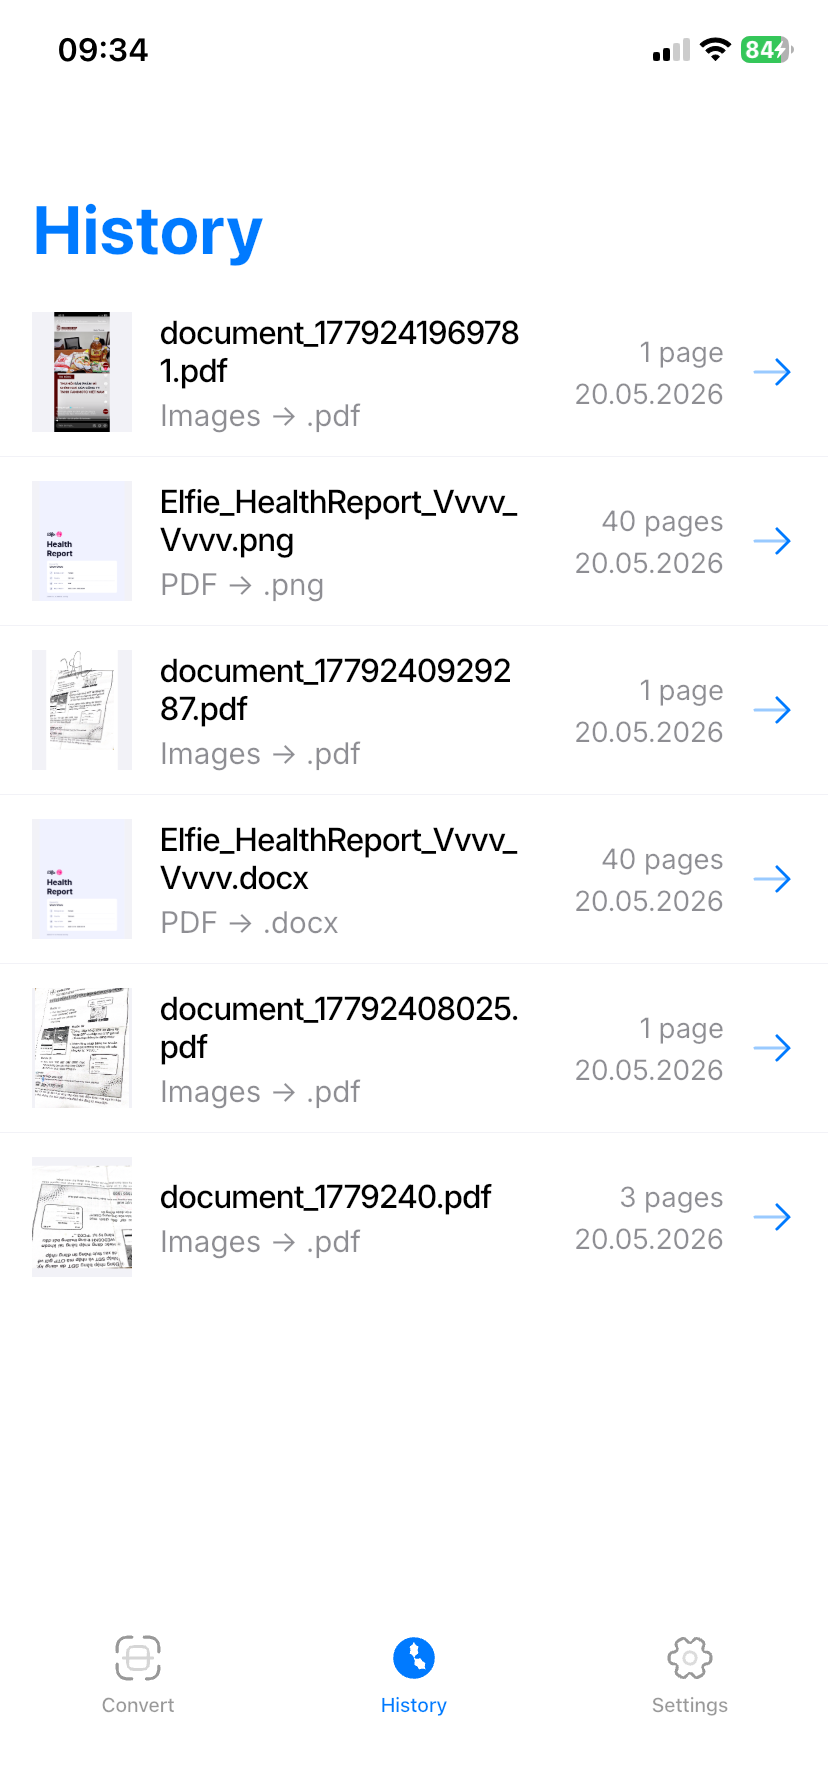
\includegraphics[height=9.5cm]{features/IMG_7577.PNG}
        \caption{Màn hình History: lịch sử toàn bộ tài liệu đã chuyển đổi kèm thumbnail, tên tệp, định dạng nguồn$\rightarrow$đích, số trang và ngày giờ (Isar DB).}
        \label{fig:pdf_history}
    \end{minipage}
\end{figure}

\newpage
\subsubsection*{3.6. Cài đặt ứng dụng và Đa ngôn ngữ}
\begin{figure}[htbp]
    \centering
    \begin{minipage}{0.45\textwidth}
        \centering
        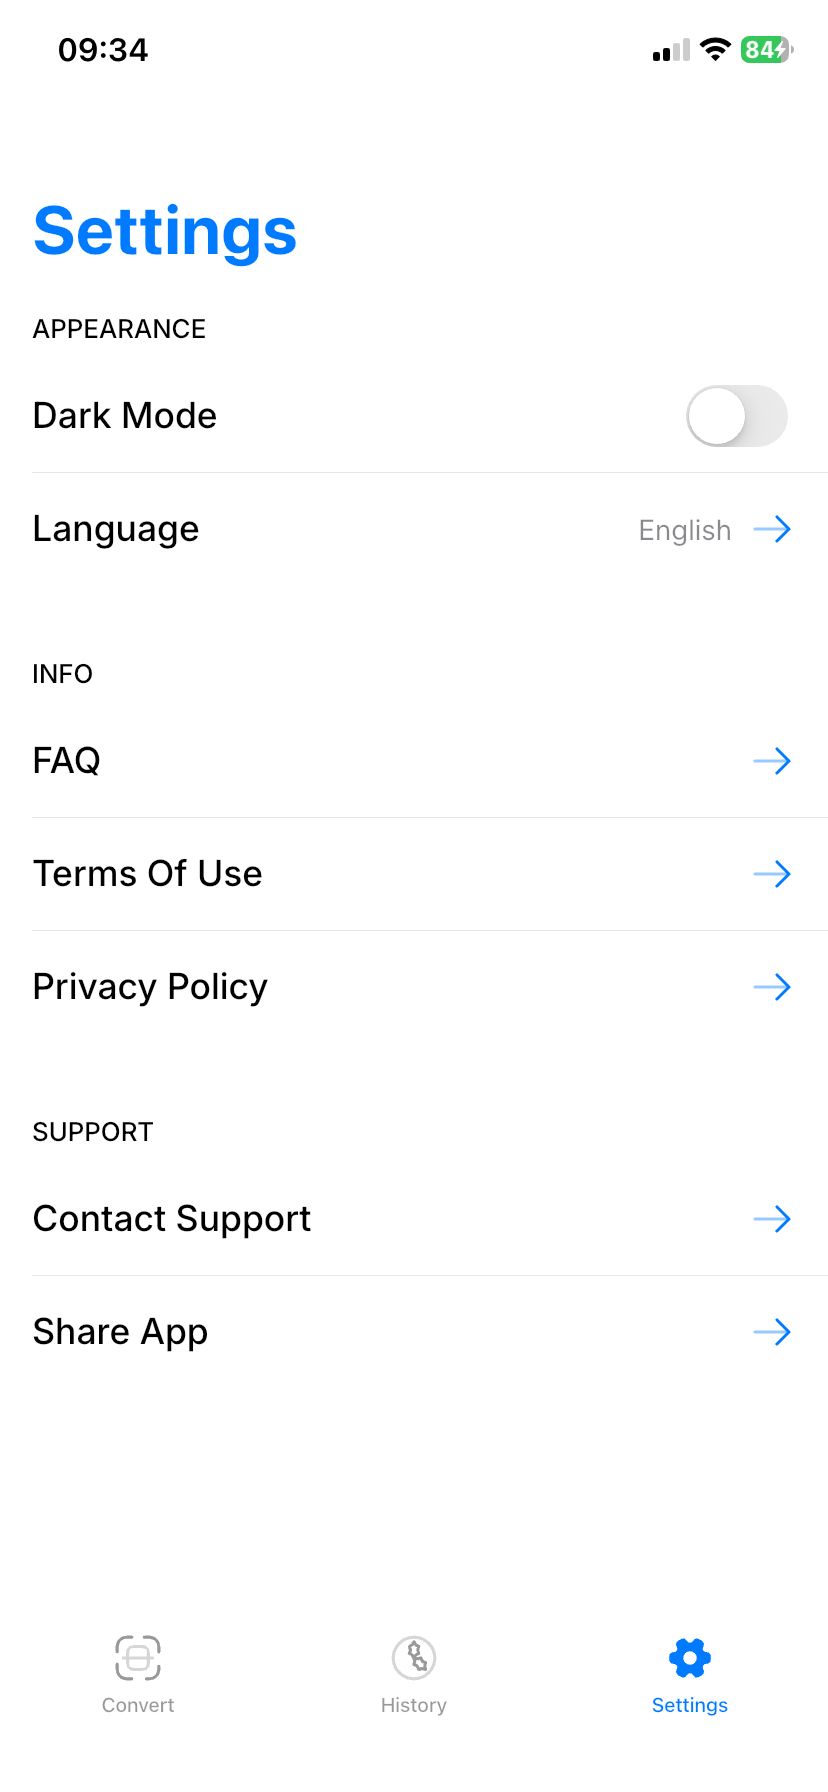
\includegraphics[height=9.5cm]{features/IMG_7578.PNG}
        \caption{Màn hình Settings: tùy chỉnh Dark Mode, Language, FAQ, Terms Of Use, Privacy Policy, Contact Support, Share App.}
        \label{fig:pdf_settings}
    \end{minipage}
    \hfill
    \begin{minipage}{0.45\textwidth}
        \centering
        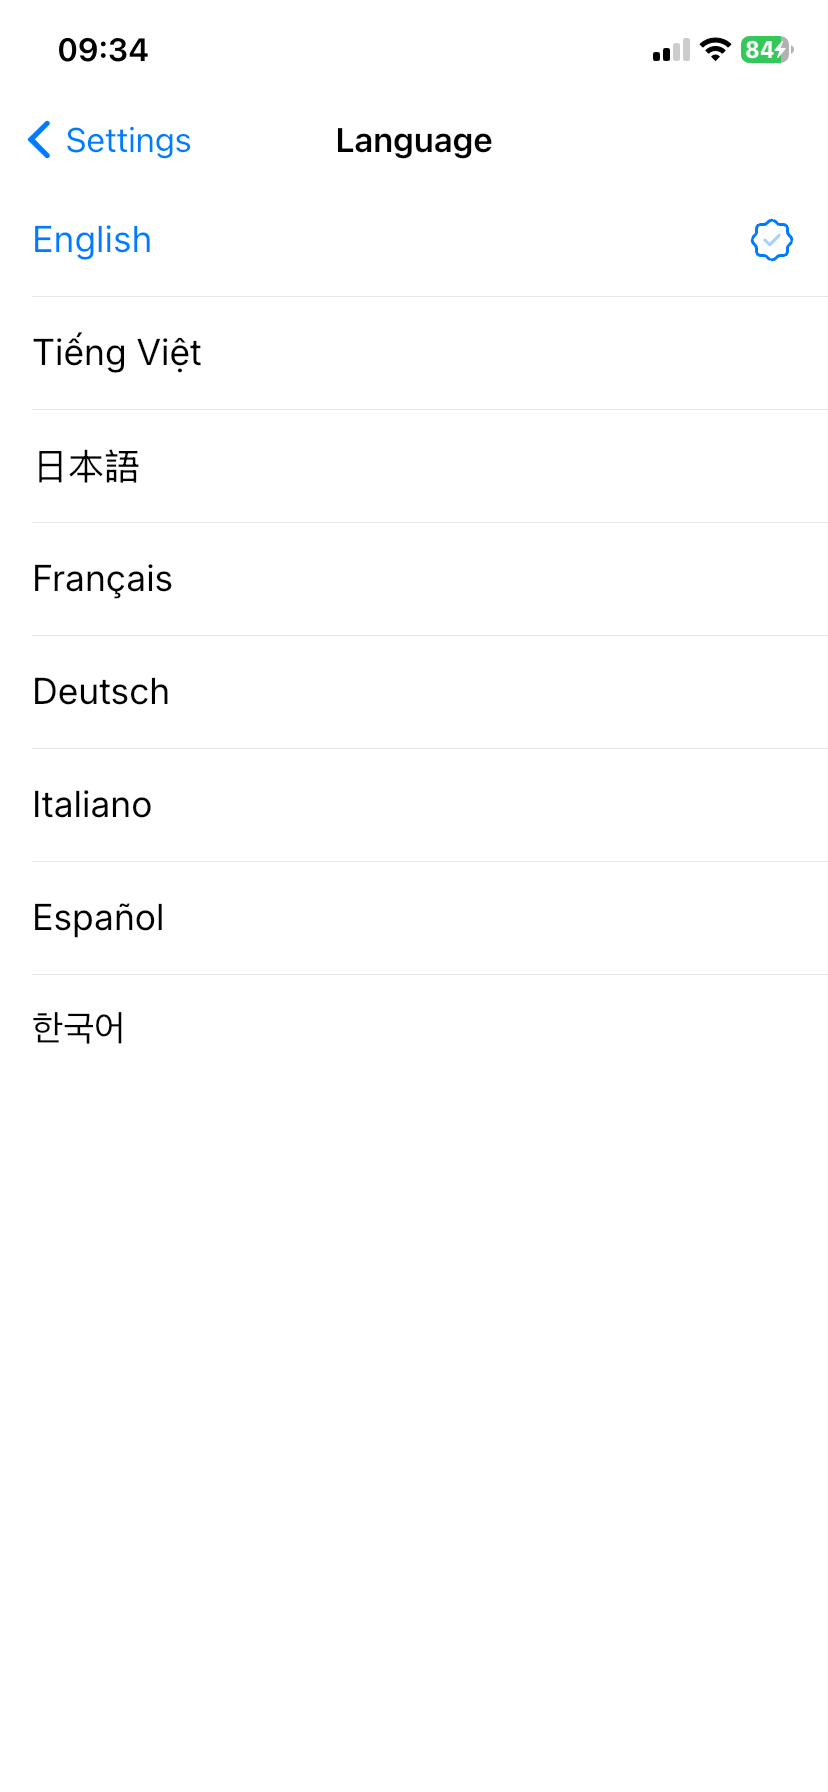
\includegraphics[height=9.5cm]{features/IMG_7579.PNG}
        \caption{Màn hình Language: hỗ trợ 8 ngôn ngữ giao diện (English, Tiếng Việt, Japanese, Français, Deutsch, Italiano, Español, Korean).}
        \label{fig:pdf_language}
    \end{minipage}
\end{figure}

\newpage
\subsection*{Phần 4: Dự án Ad-Free Blood Pressure App (Giai đoạn 4)}
Ứng dụng tự phát triển và phát hành thành công trên App Store:

\begin{figure}[htbp]
    \centering
    \begin{minipage}{0.45\textwidth}
        \centering
        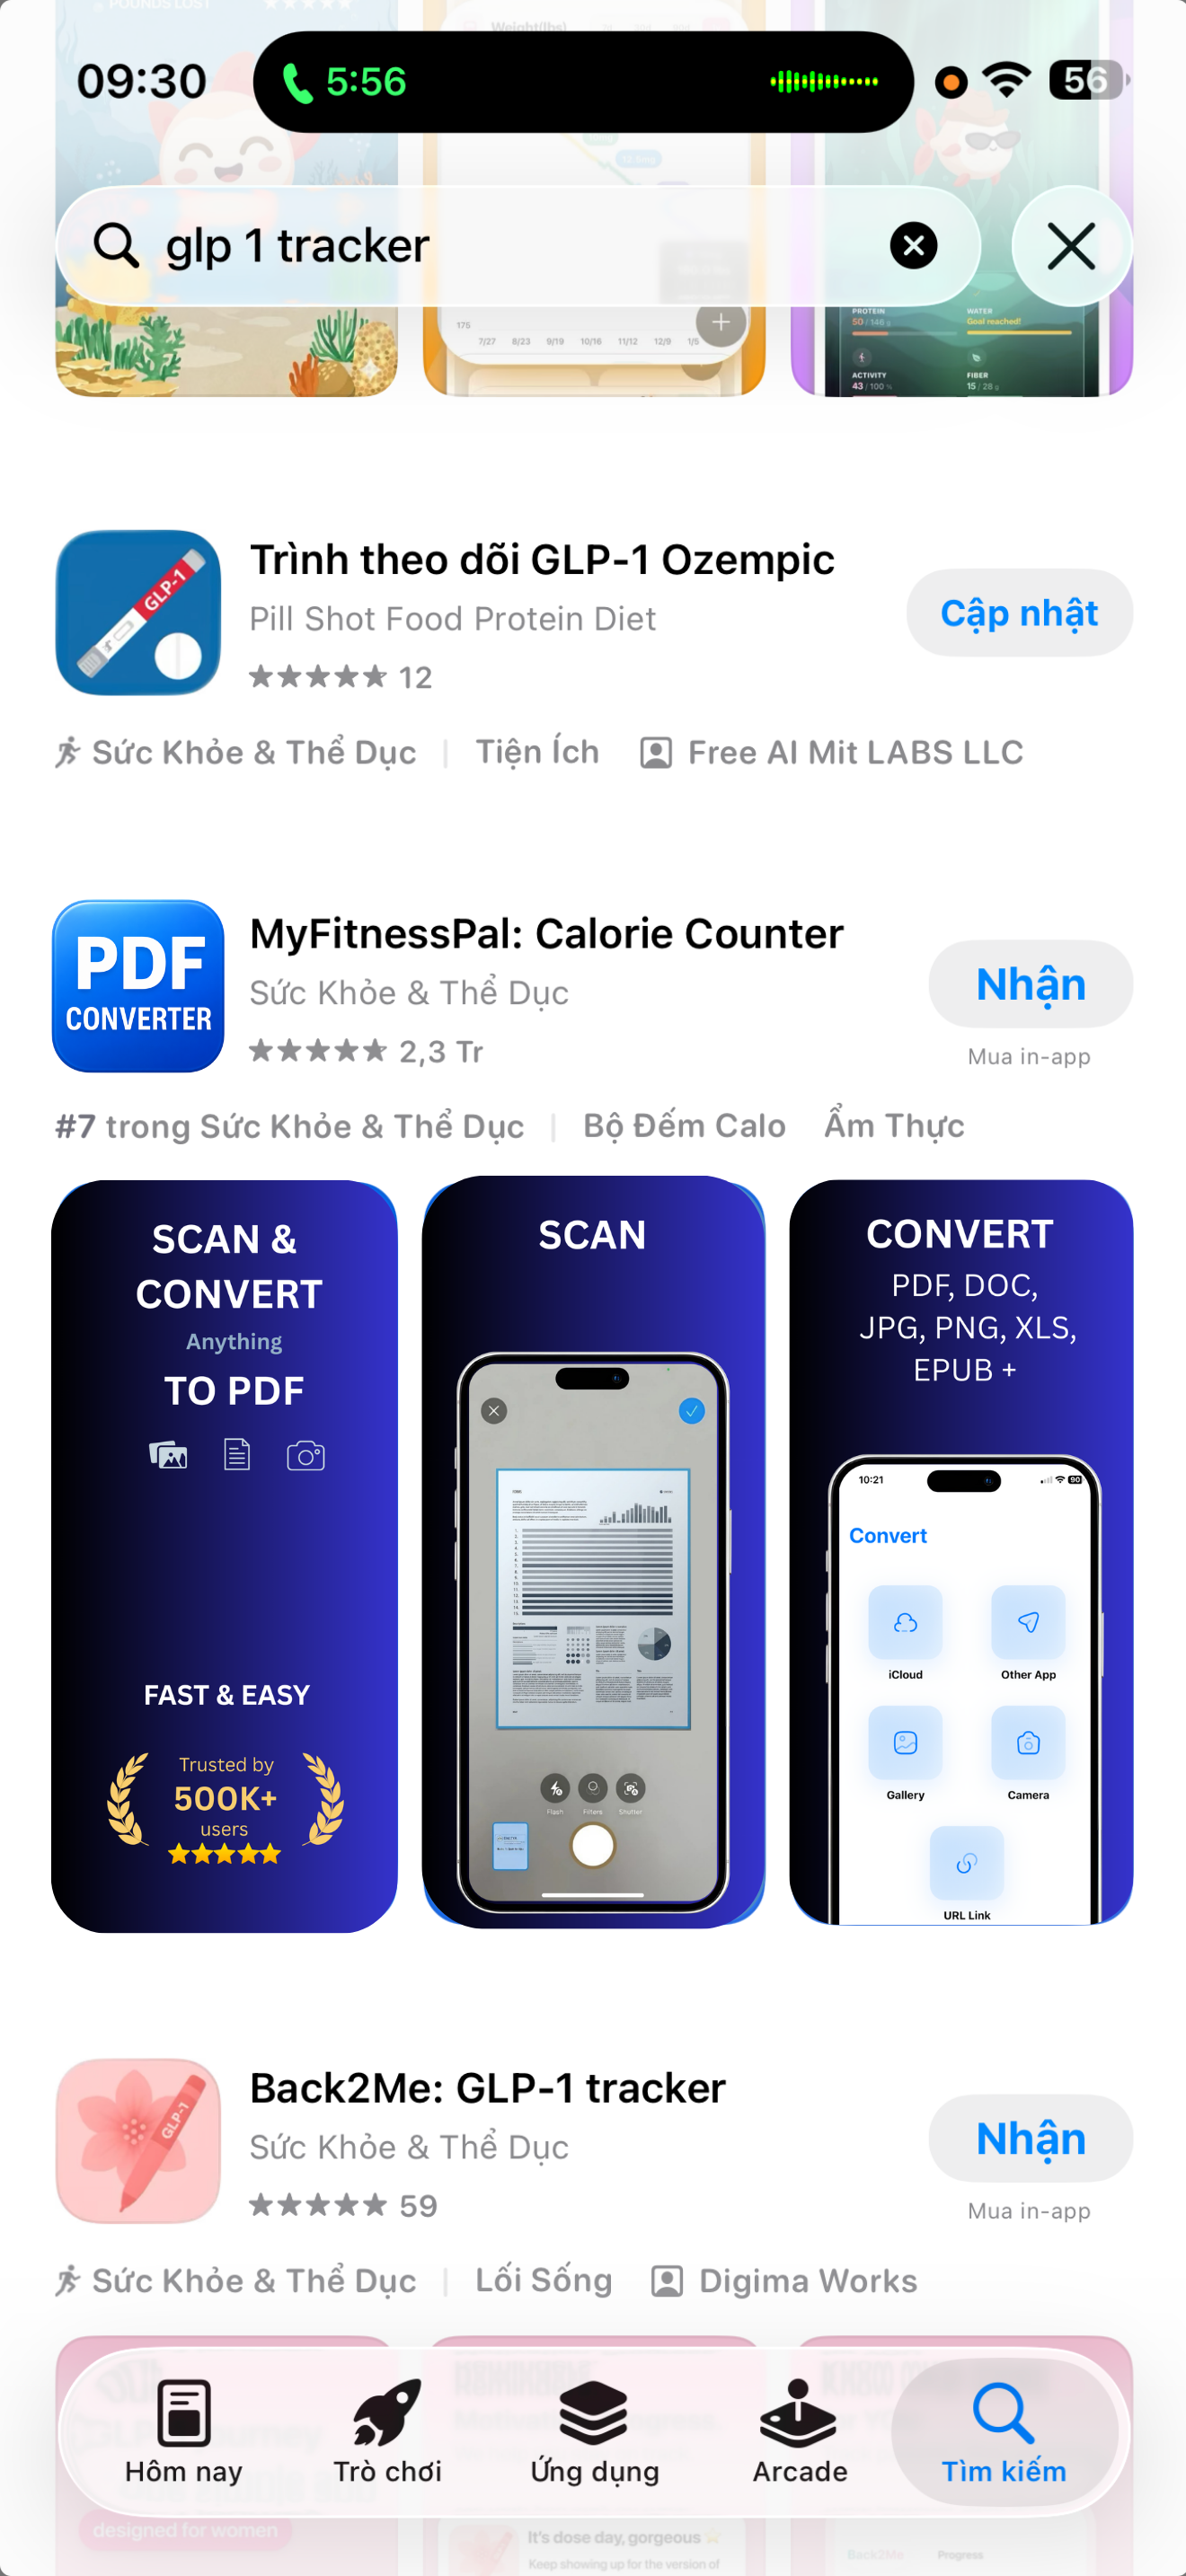
\includegraphics[width=\textwidth]{demo_app_store/1.png}\\
        \vspace{0.1cm}
        \scriptsize Giao diện App Store (Chế độ Sáng)
    \end{minipage}
    \hfill
    \begin{minipage}{0.45\textwidth}
        \centering
        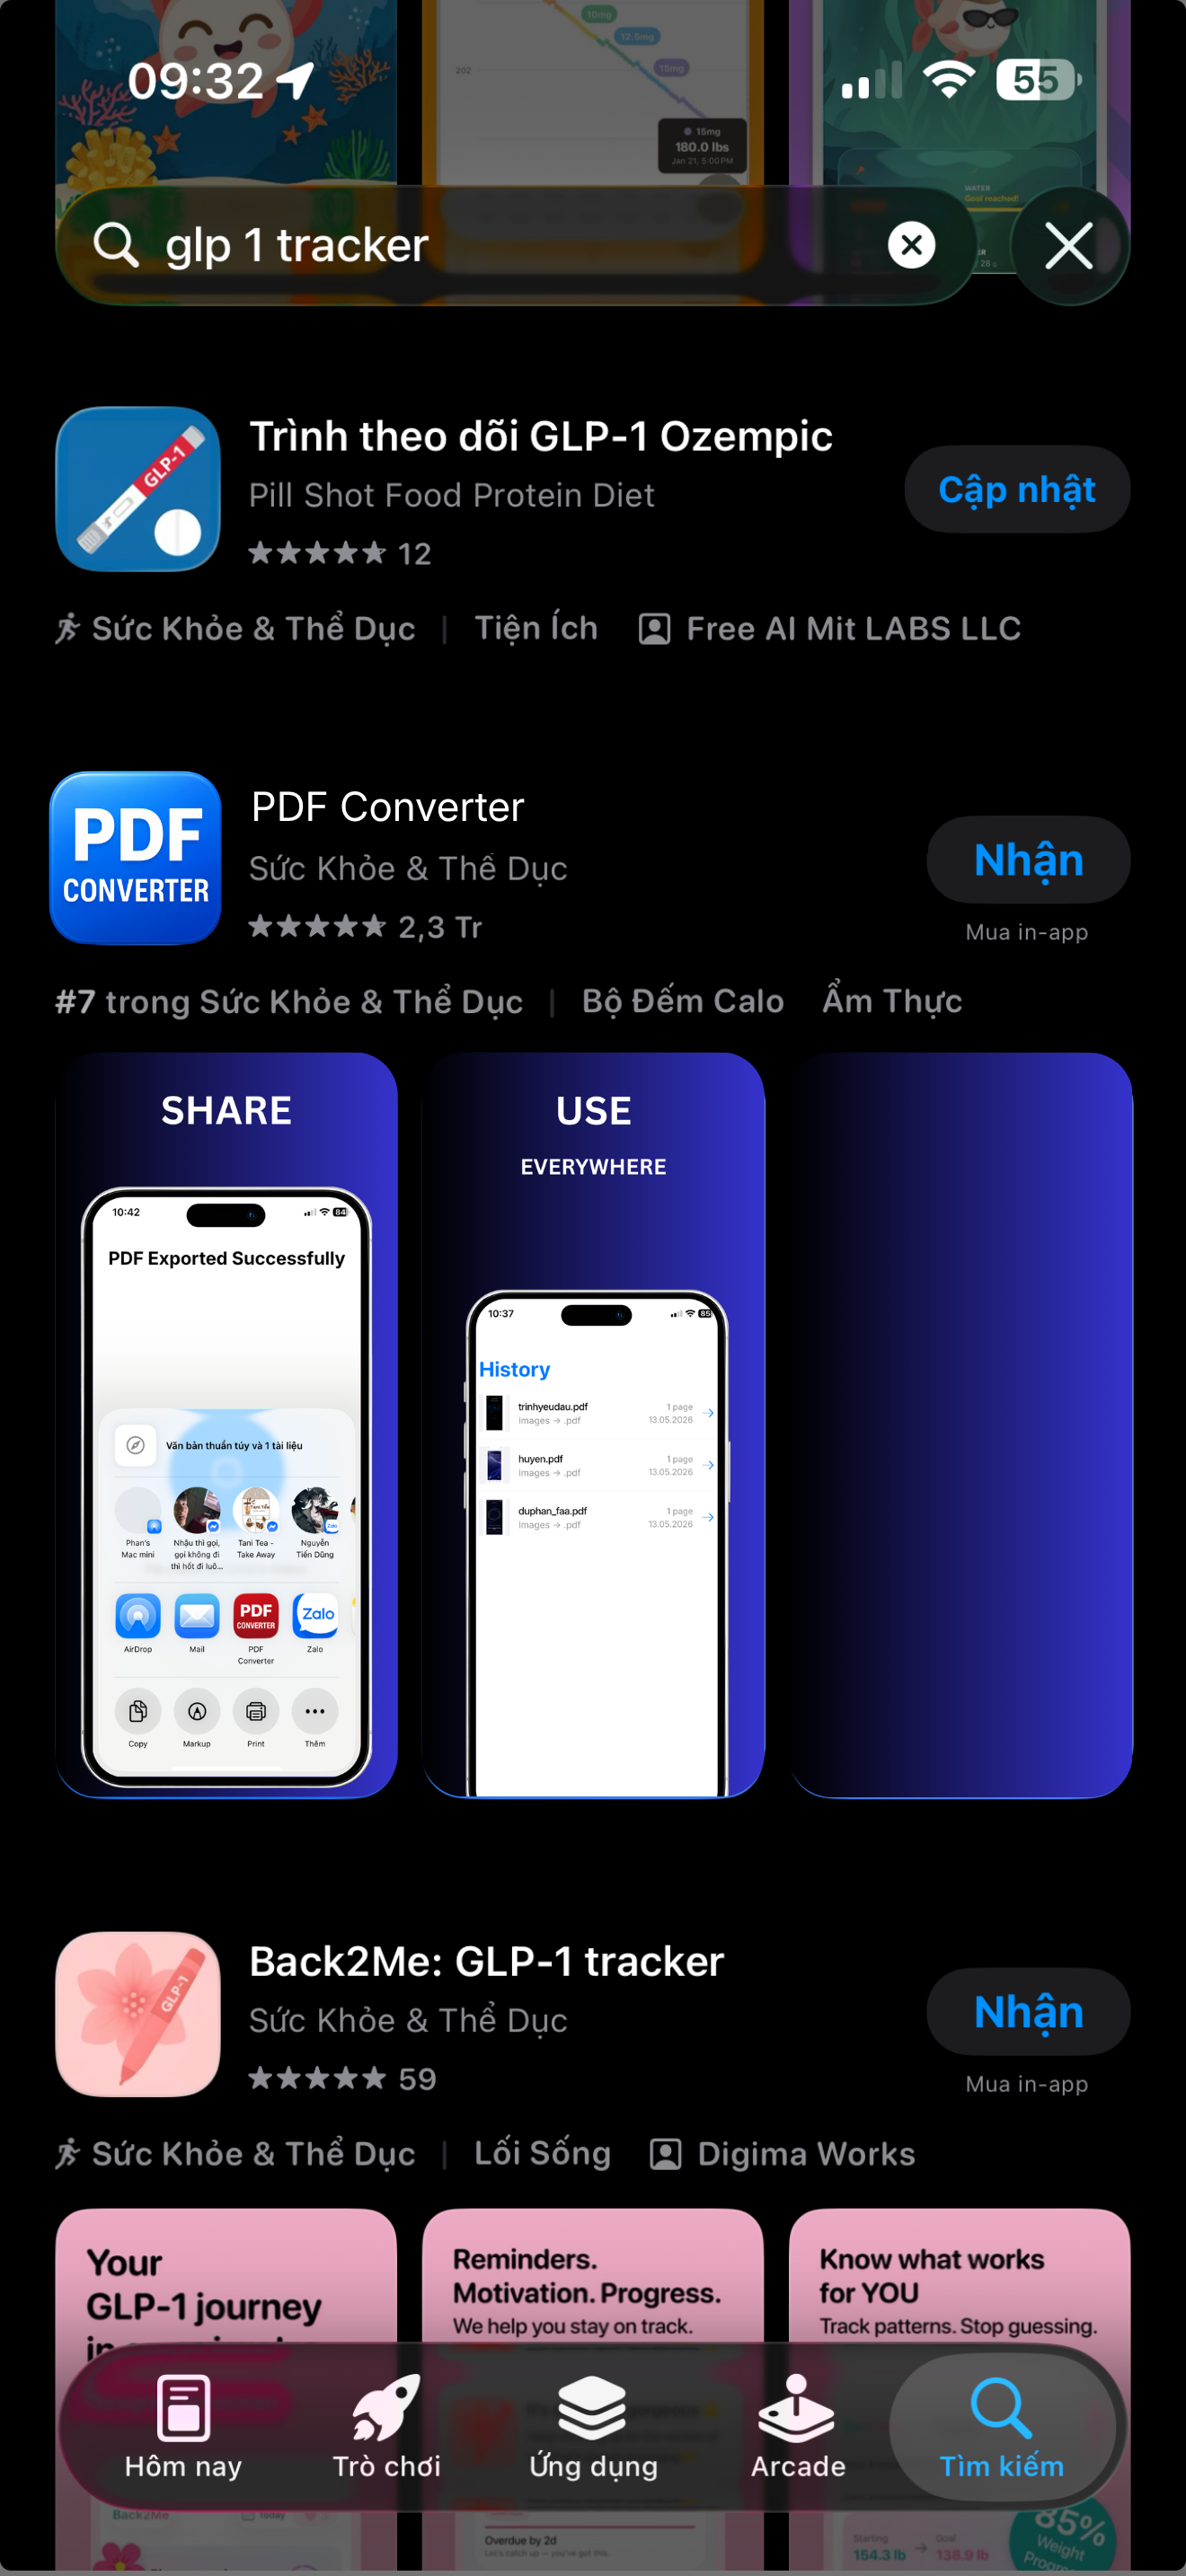
\includegraphics[width=\textwidth]{demo_app_store/2.png}\\
        \vspace{0.1cm}
        \scriptsize Giao diện App Store (Chế độ Tối)
    \end{minipage}
\end{figure}

\end{document}
